\documentclass[a4paper,11pt,aps,secnumarabic,balancelastpage,amsmath,amssymb,floatfix,table]{article}
\usepackage{packages}
\usepackage[backend=biber,style=numeric,sorting=none]{biblatex}
\addbibresource{references.bib}



\begin{document}

\title{\bf{Measurements Burridge-Knopoff oscillators}}
\author{Bitto Manuel}
\date{\today}
\maketitle

\section{Single block measurements}

\subsection{Breadboard implementation}\label{sec:breadboard}

The inductorless electronic analog of the Burridge-Knopoff model
\cite{main_paper} is represented in Fig.
\ref{fig:breadboard implementation}. This circuit was implemented
in a breadboard using 1N5817 Schottky diodes and different kinds
of op-amps, namely UA741, OP07, TL081 and OP27; these op-amps were
supplied with $V_{CC}=\pm12~\text{V}$. The nominal values for the
resistances and capacitors are $R=R_c=10~\text{k}\Omega$,
$R_A=R_B=10~\text{k}\Omega$, $r=1.8~\text{k}\Omega$ and
$C=100~\text{nF}$. The input voltages are $V_0=1~\text{V}$ and
the variable voltage $V_d$, while the output voltages are
$V$ and $W$ (the subscript $i$ is omitted).

The oscillating behavior of this circuit is shown in Fig.
\ref{fig:oscillation breadboard}. The lower clamping in the Lissajous
figure is intended and is due to the presence of the Schottky diodes.
The frequency behavior at high voltages,
namely $V_d \gtrsim 1$ V, is the same for each kind of op-amp.
On the other hand, the amplitudes possess an offset which depends on
the selected op-amp; nonetheless, they all exhibit a mostly linear
behavior.

\begin{figure}[H]
    \centering
    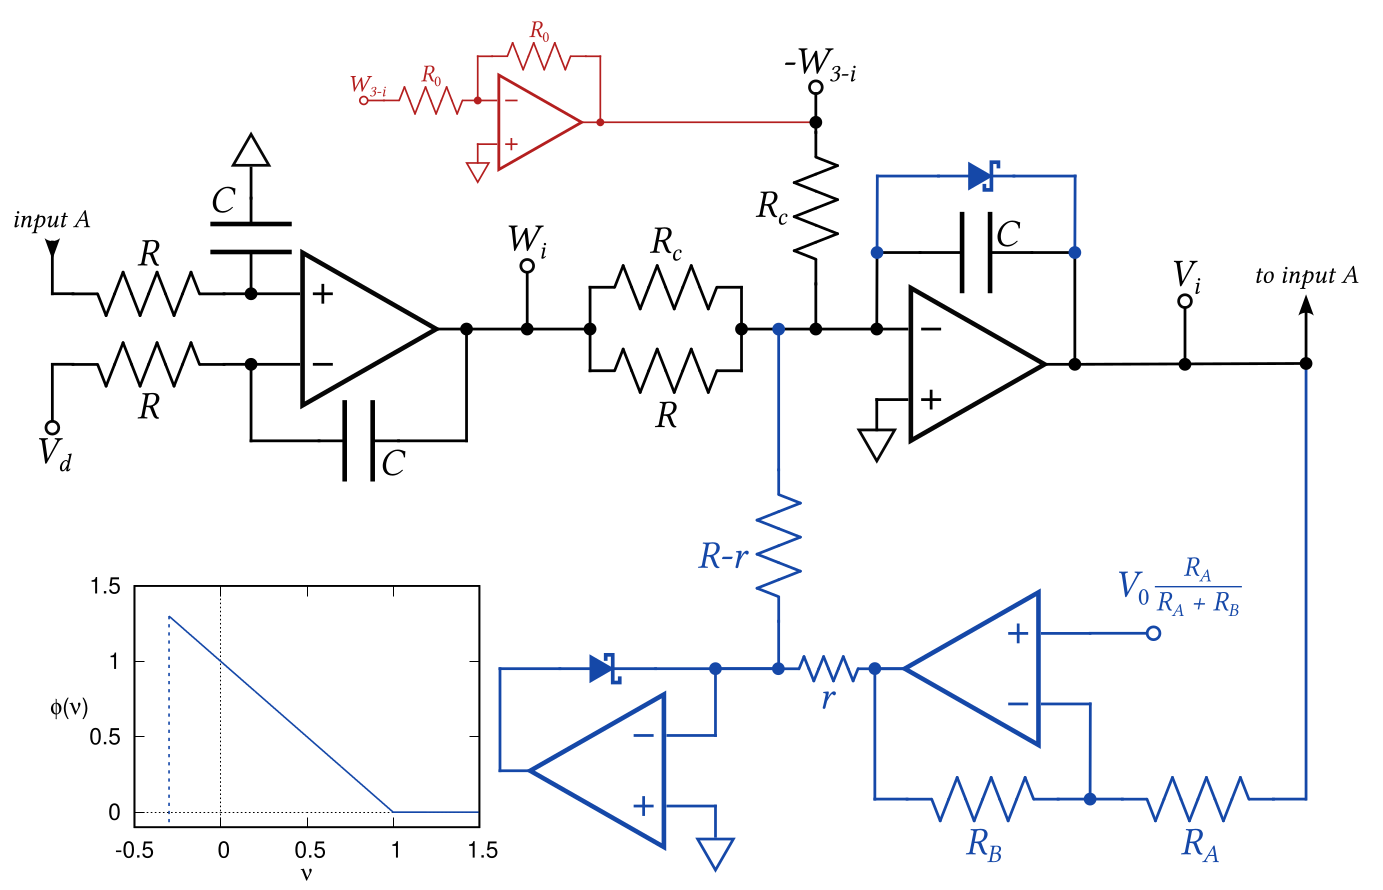
\includegraphics[width=\linewidth]
    {../1_block/breadboard/breadboard_implementation.png}
    \caption{Inductorless representation of the BK model.
    The blue part of the network refers to the nonlinear element,
    whose characteristic is drawn in the bottom left plot.
    Figure adapted from Ref. \cite{main_paper}.}\label{fig:breadboard implementation}
\end{figure}

\begin{figure}[H]
    \centering
    \begin{minipage}{.58\textwidth}
        \begin{subfigure}{\linewidth}
            \centering
            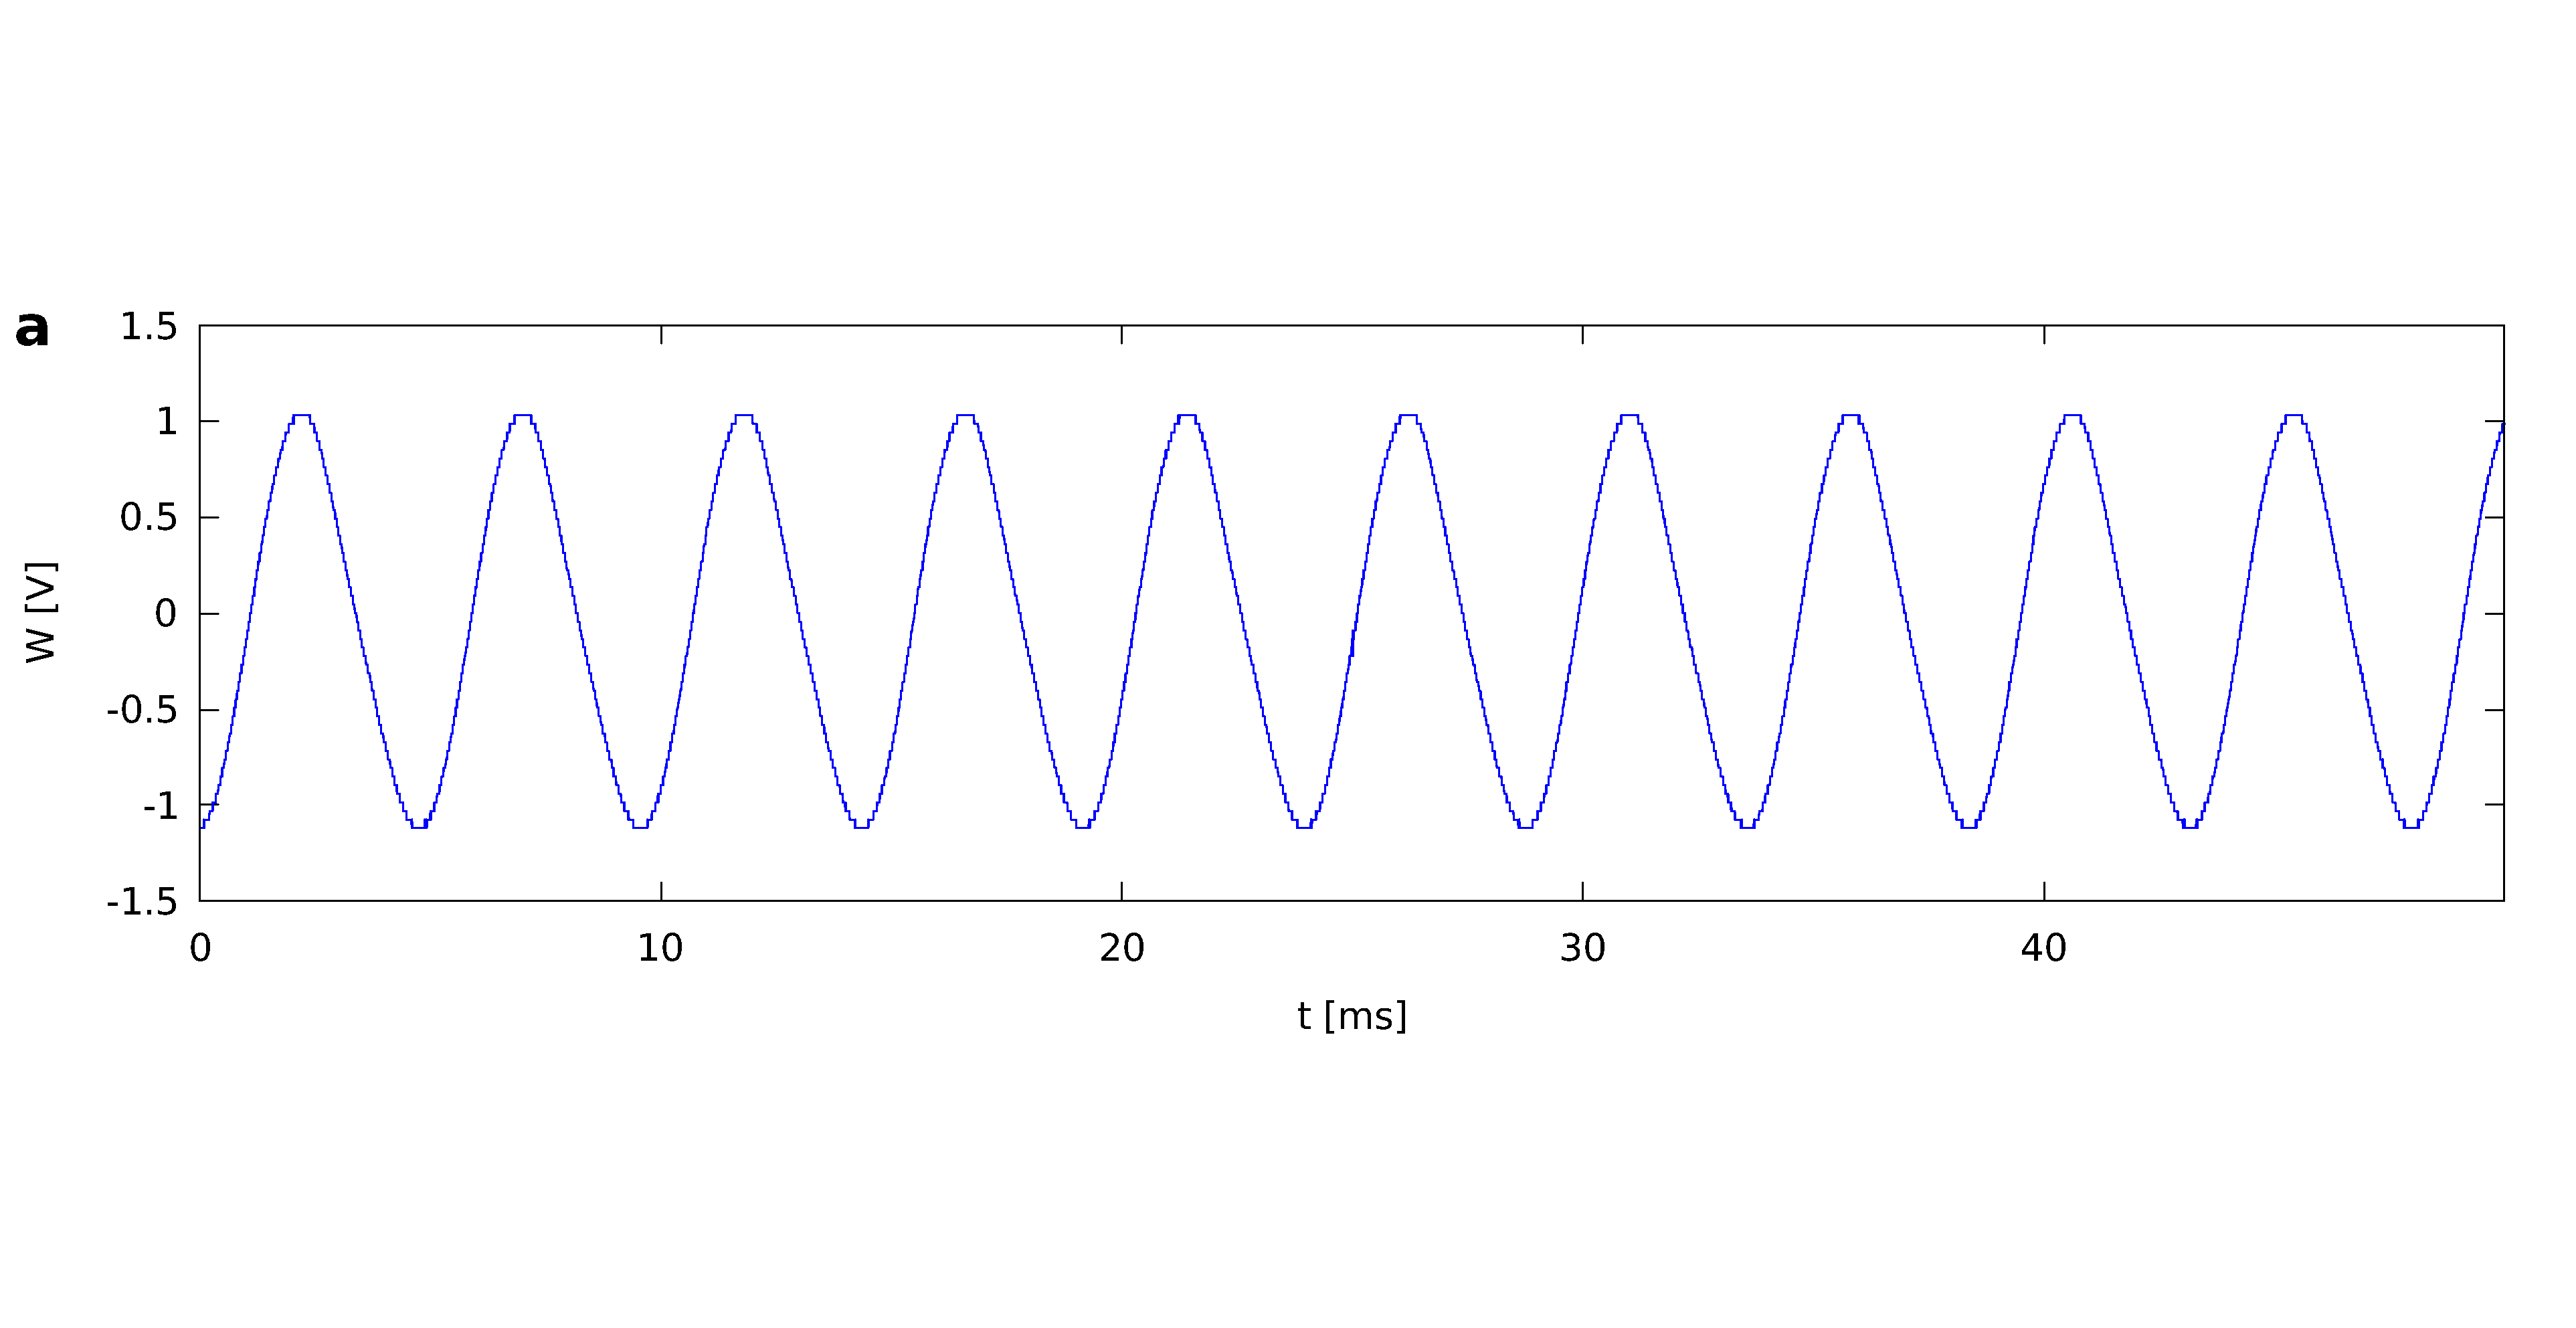
\includegraphics[width=\linewidth,trim={0 6cm 0 6cm},clip,left]
            {../1_block/breadboard/paper_implementation_op27/W_wf.pdf}\\
            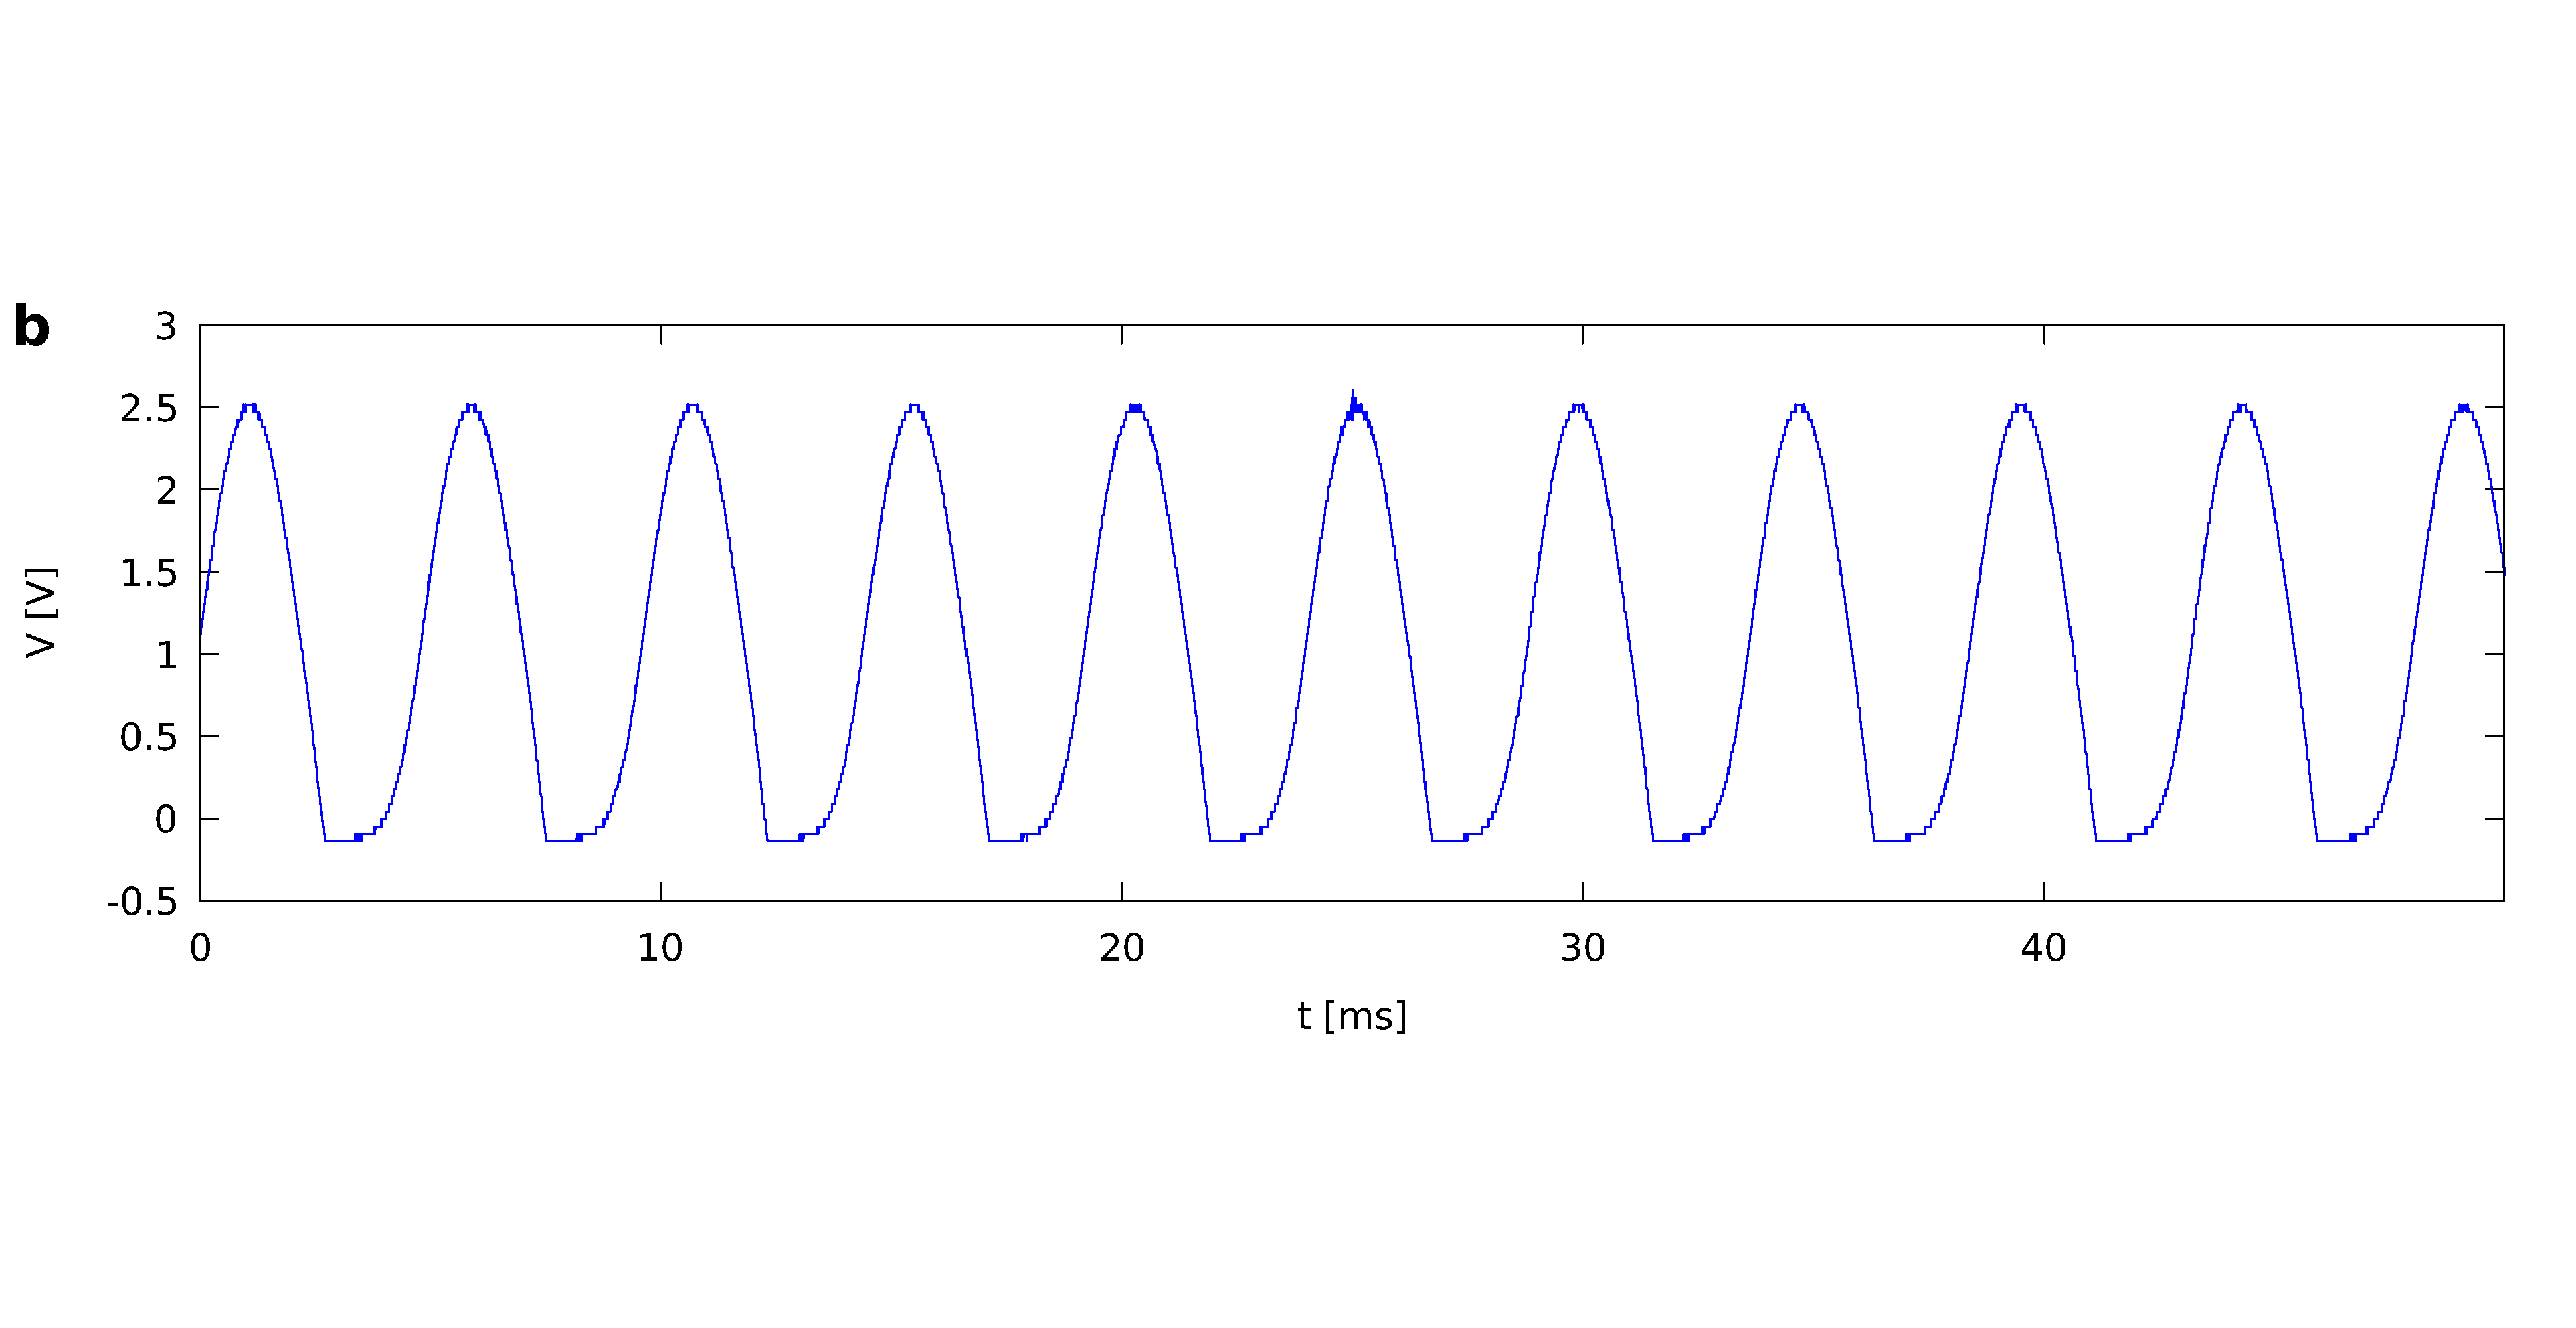
\includegraphics[width=\linewidth,trim={0 6cm 0 6cm},clip,left]
            {../1_block/breadboard/paper_implementation_op27/V_wf.pdf}
        \end{subfigure}
    \end{minipage}
    \begin{subfigure}{.39\textwidth}
        \centering
        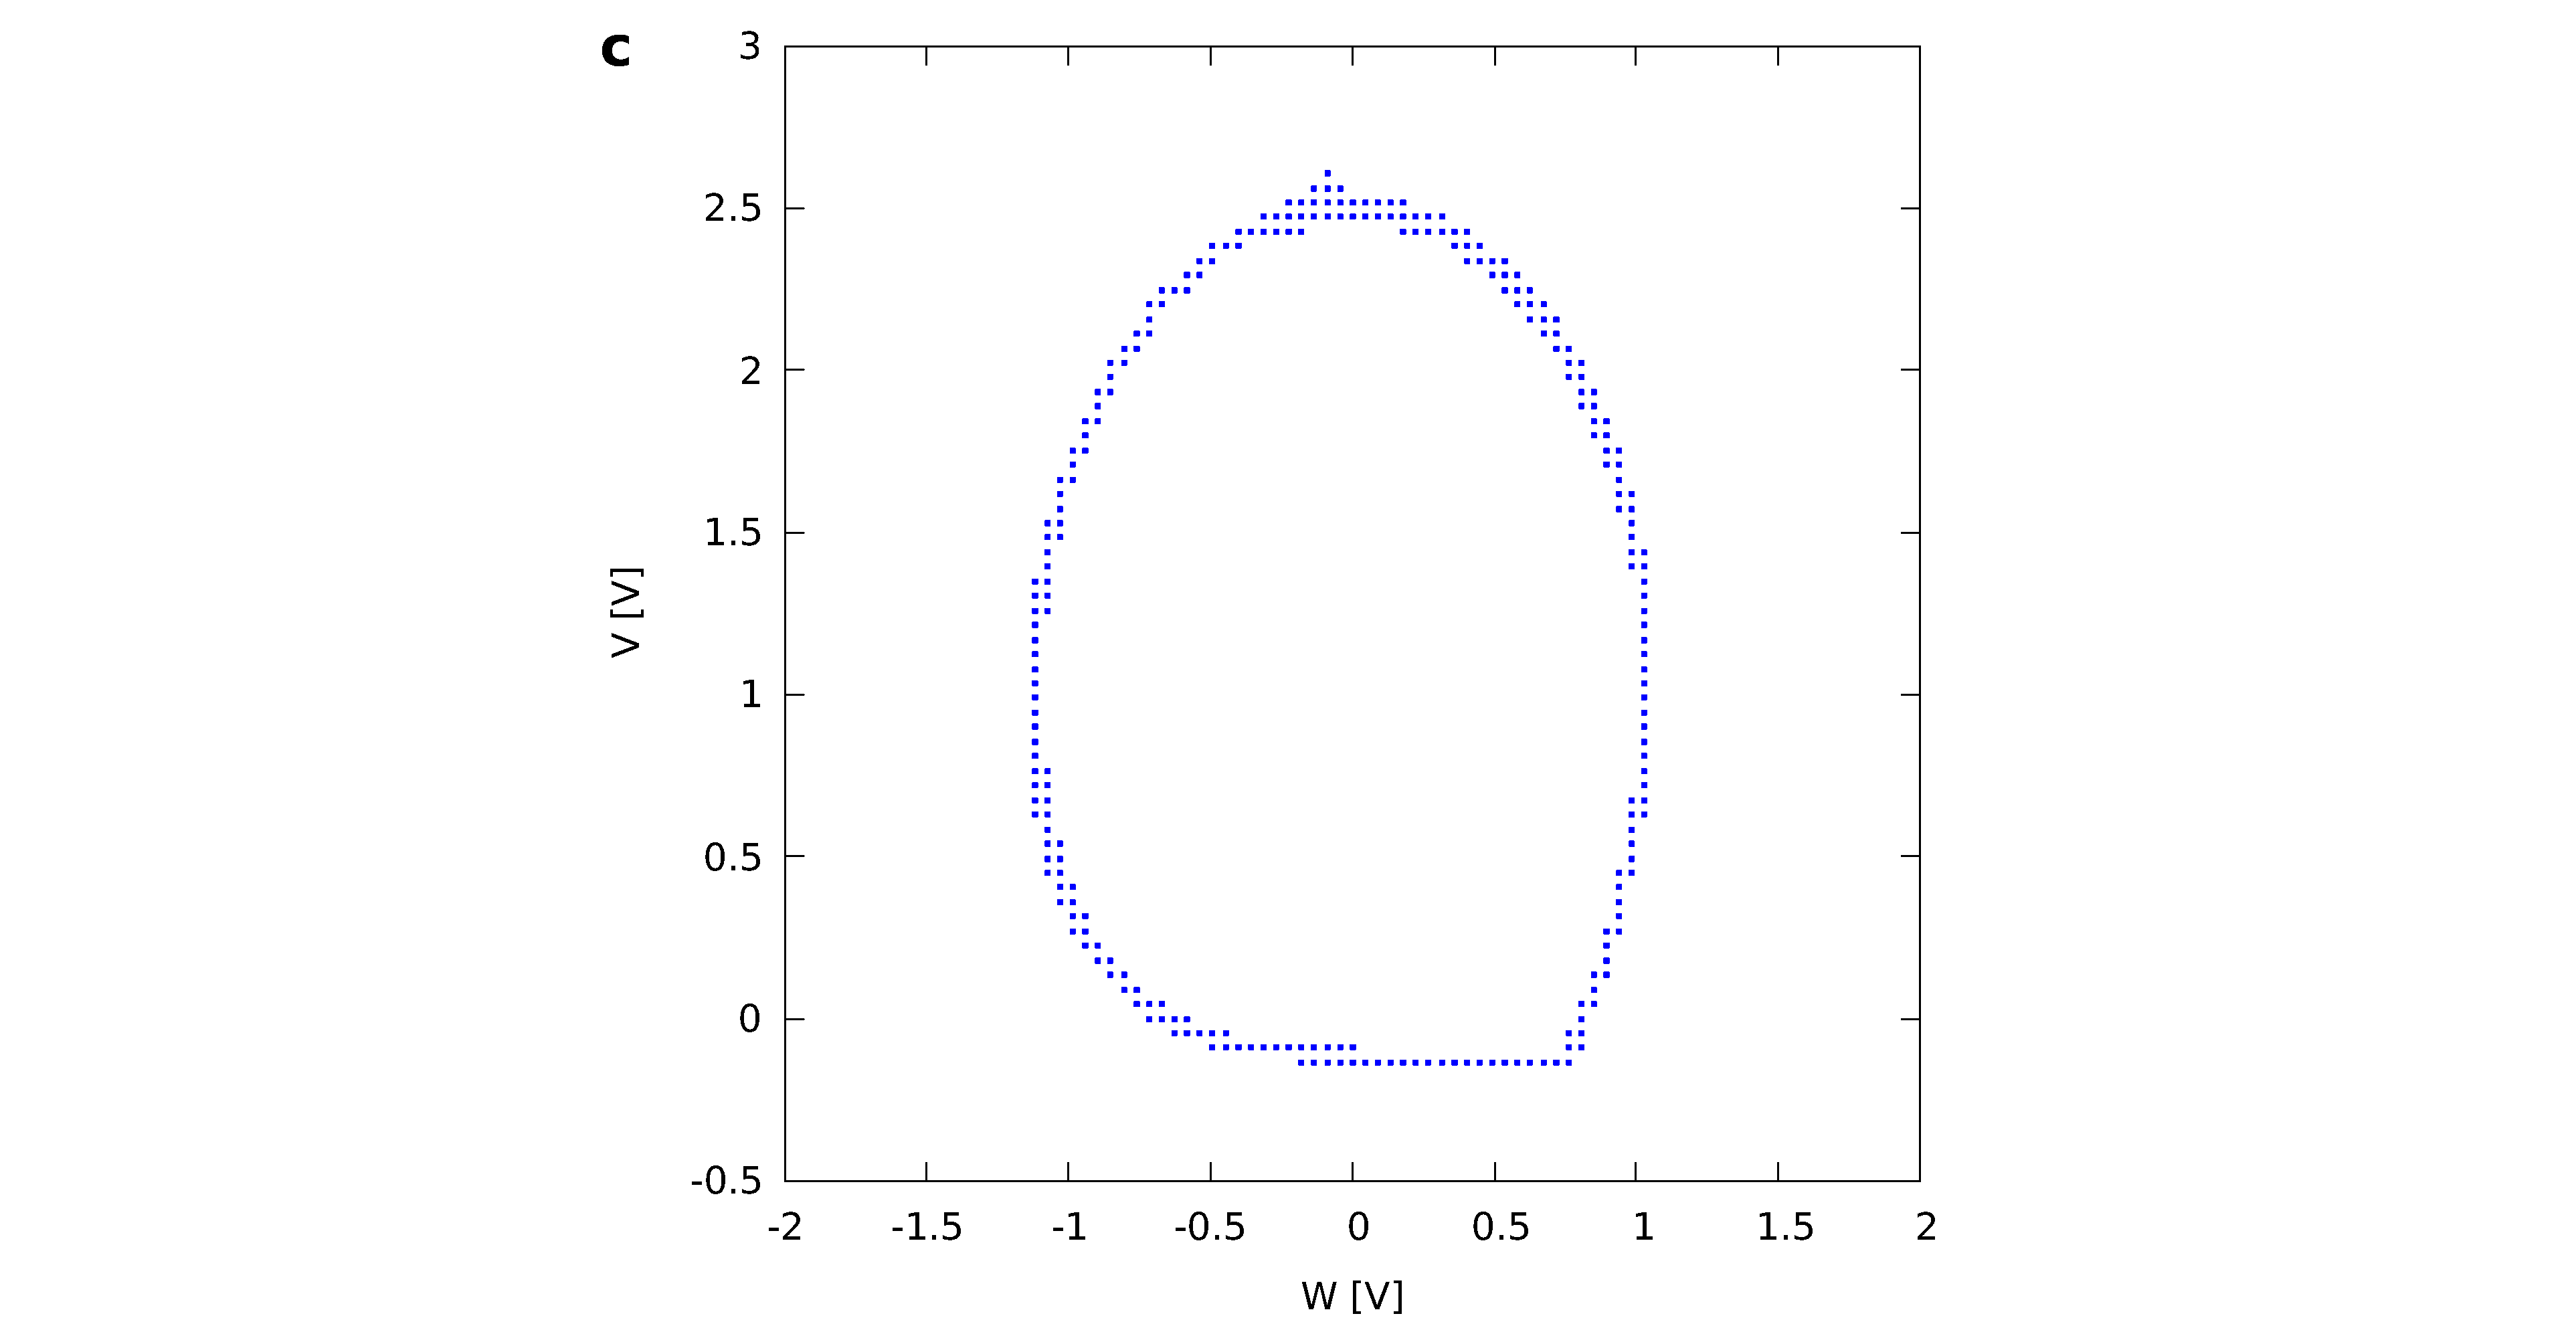
\includegraphics[width=\linewidth,trim={15cm 0 15cm 0},clip,right]
        {../1_block/breadboard/paper_implementation_op27/Lissajous.pdf}
    \end{subfigure}
    \begin{subfigure}{.49\textwidth}
        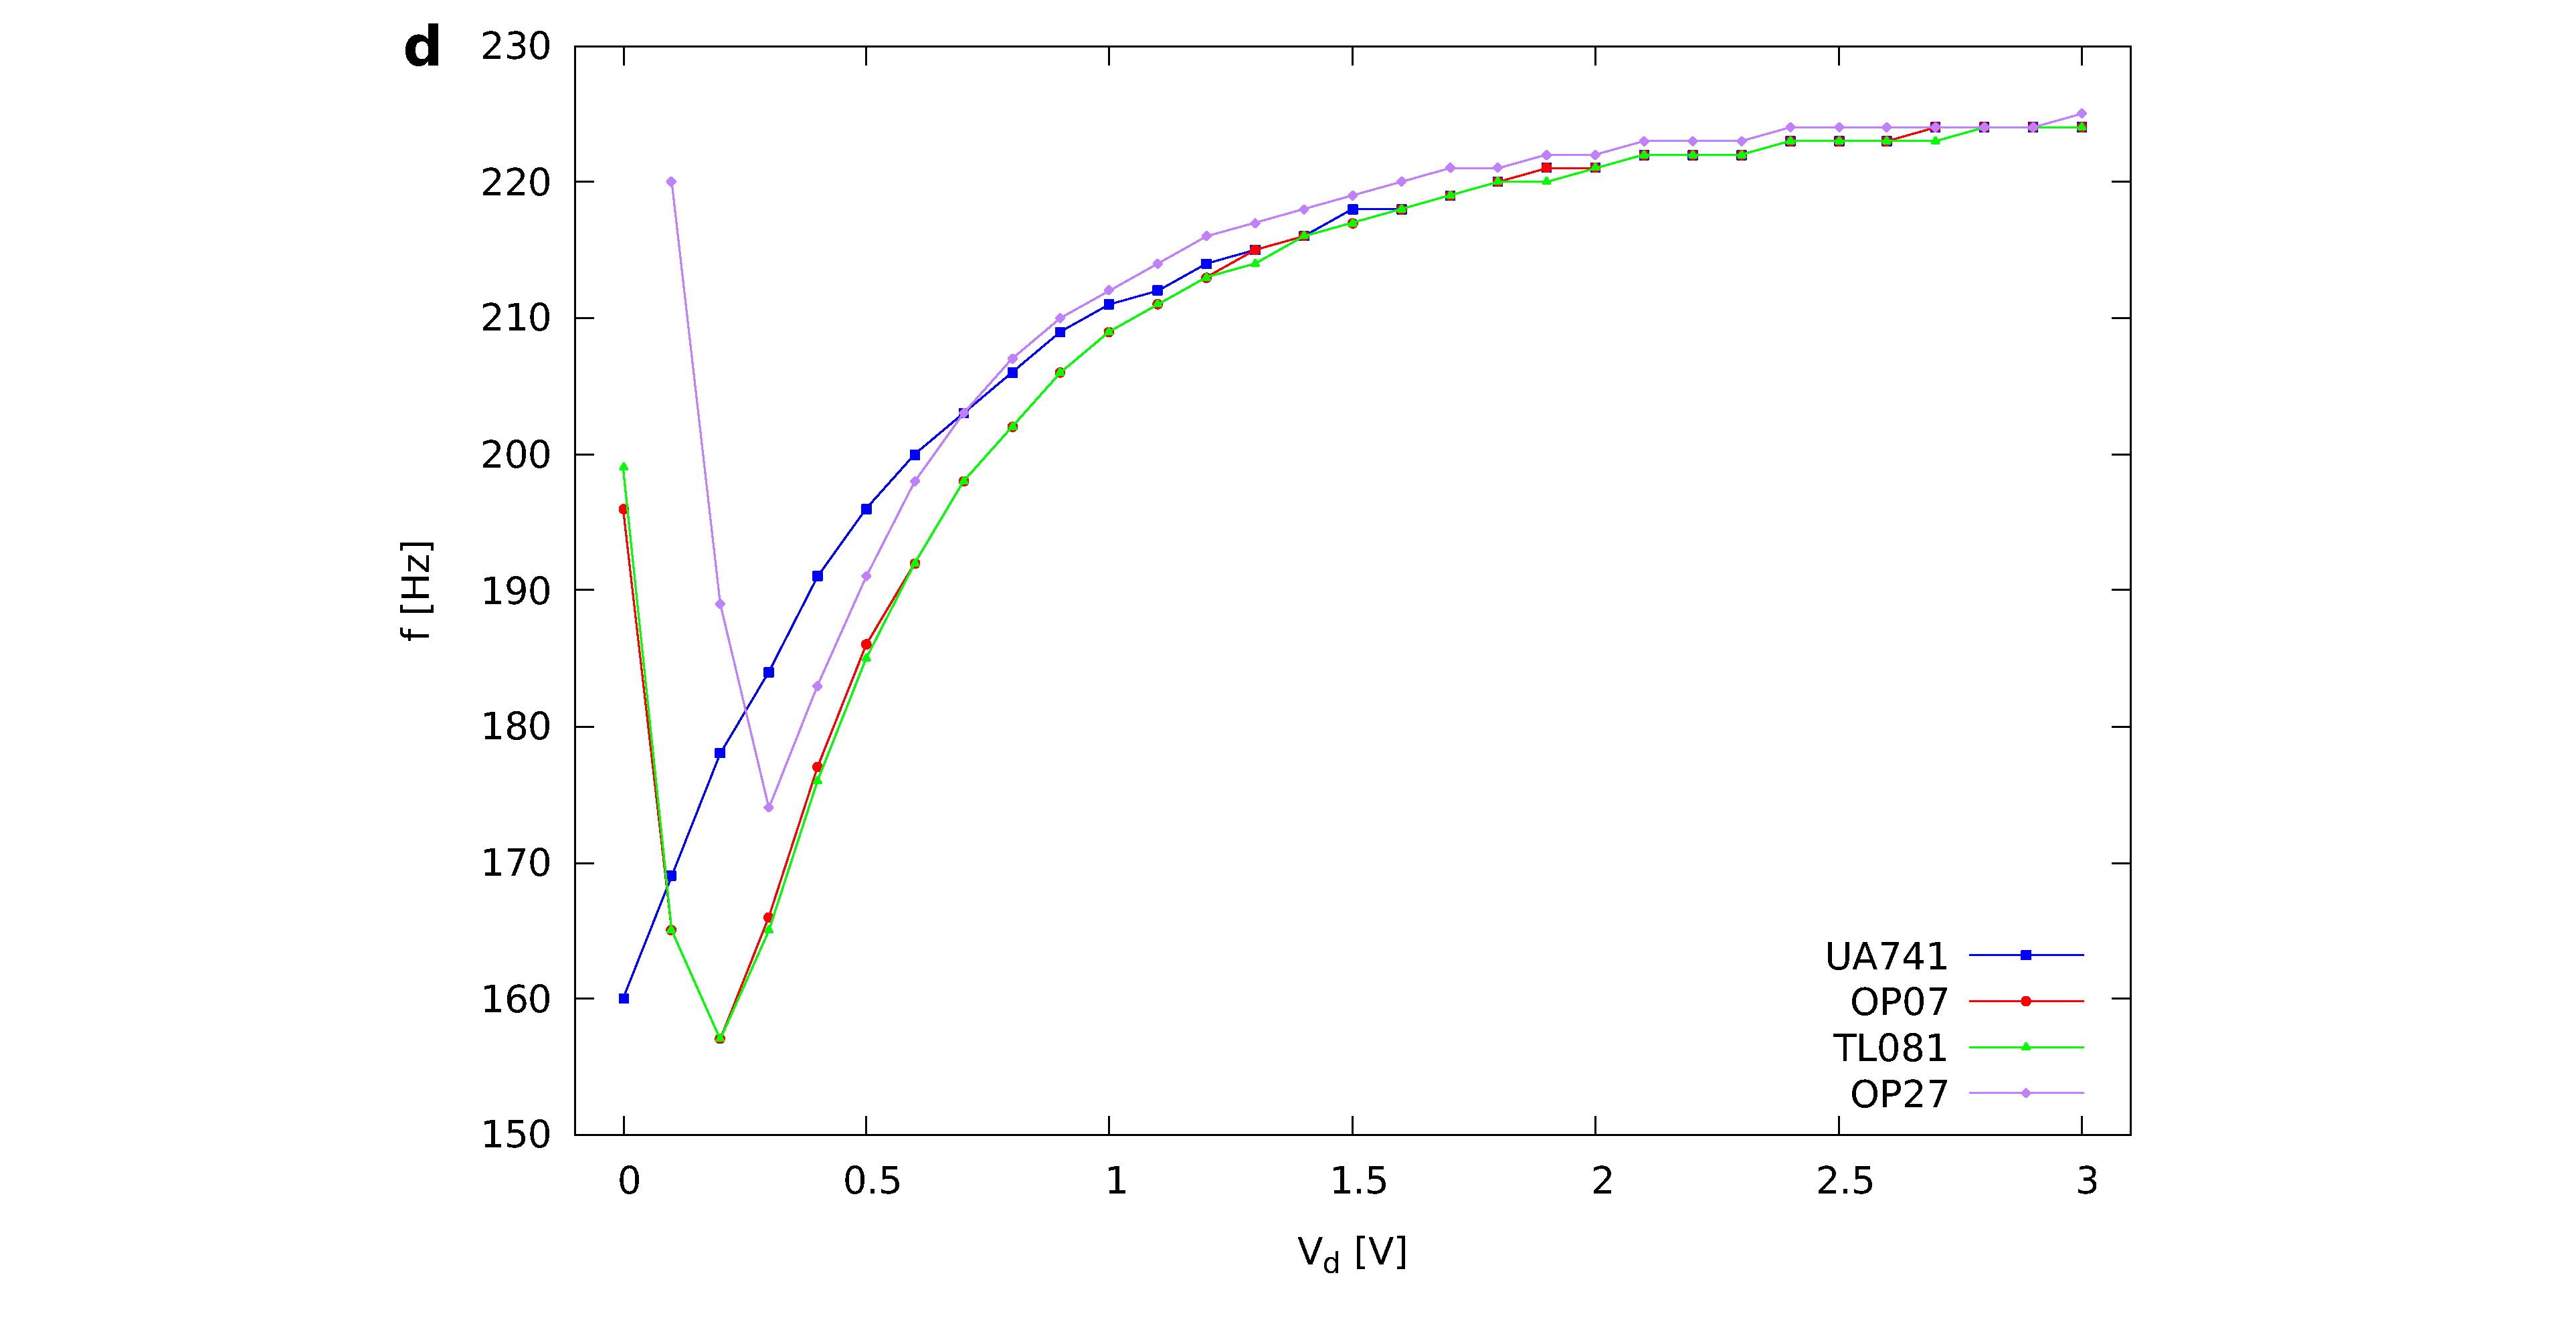
\includegraphics[width=\linewidth,trim={10cm 0 9cm 0},clip,left]
        {../1_block/breadboard/freq_bread.pdf}
    \end{subfigure}
    \begin{subfigure}{.49\textwidth}
        \centering
        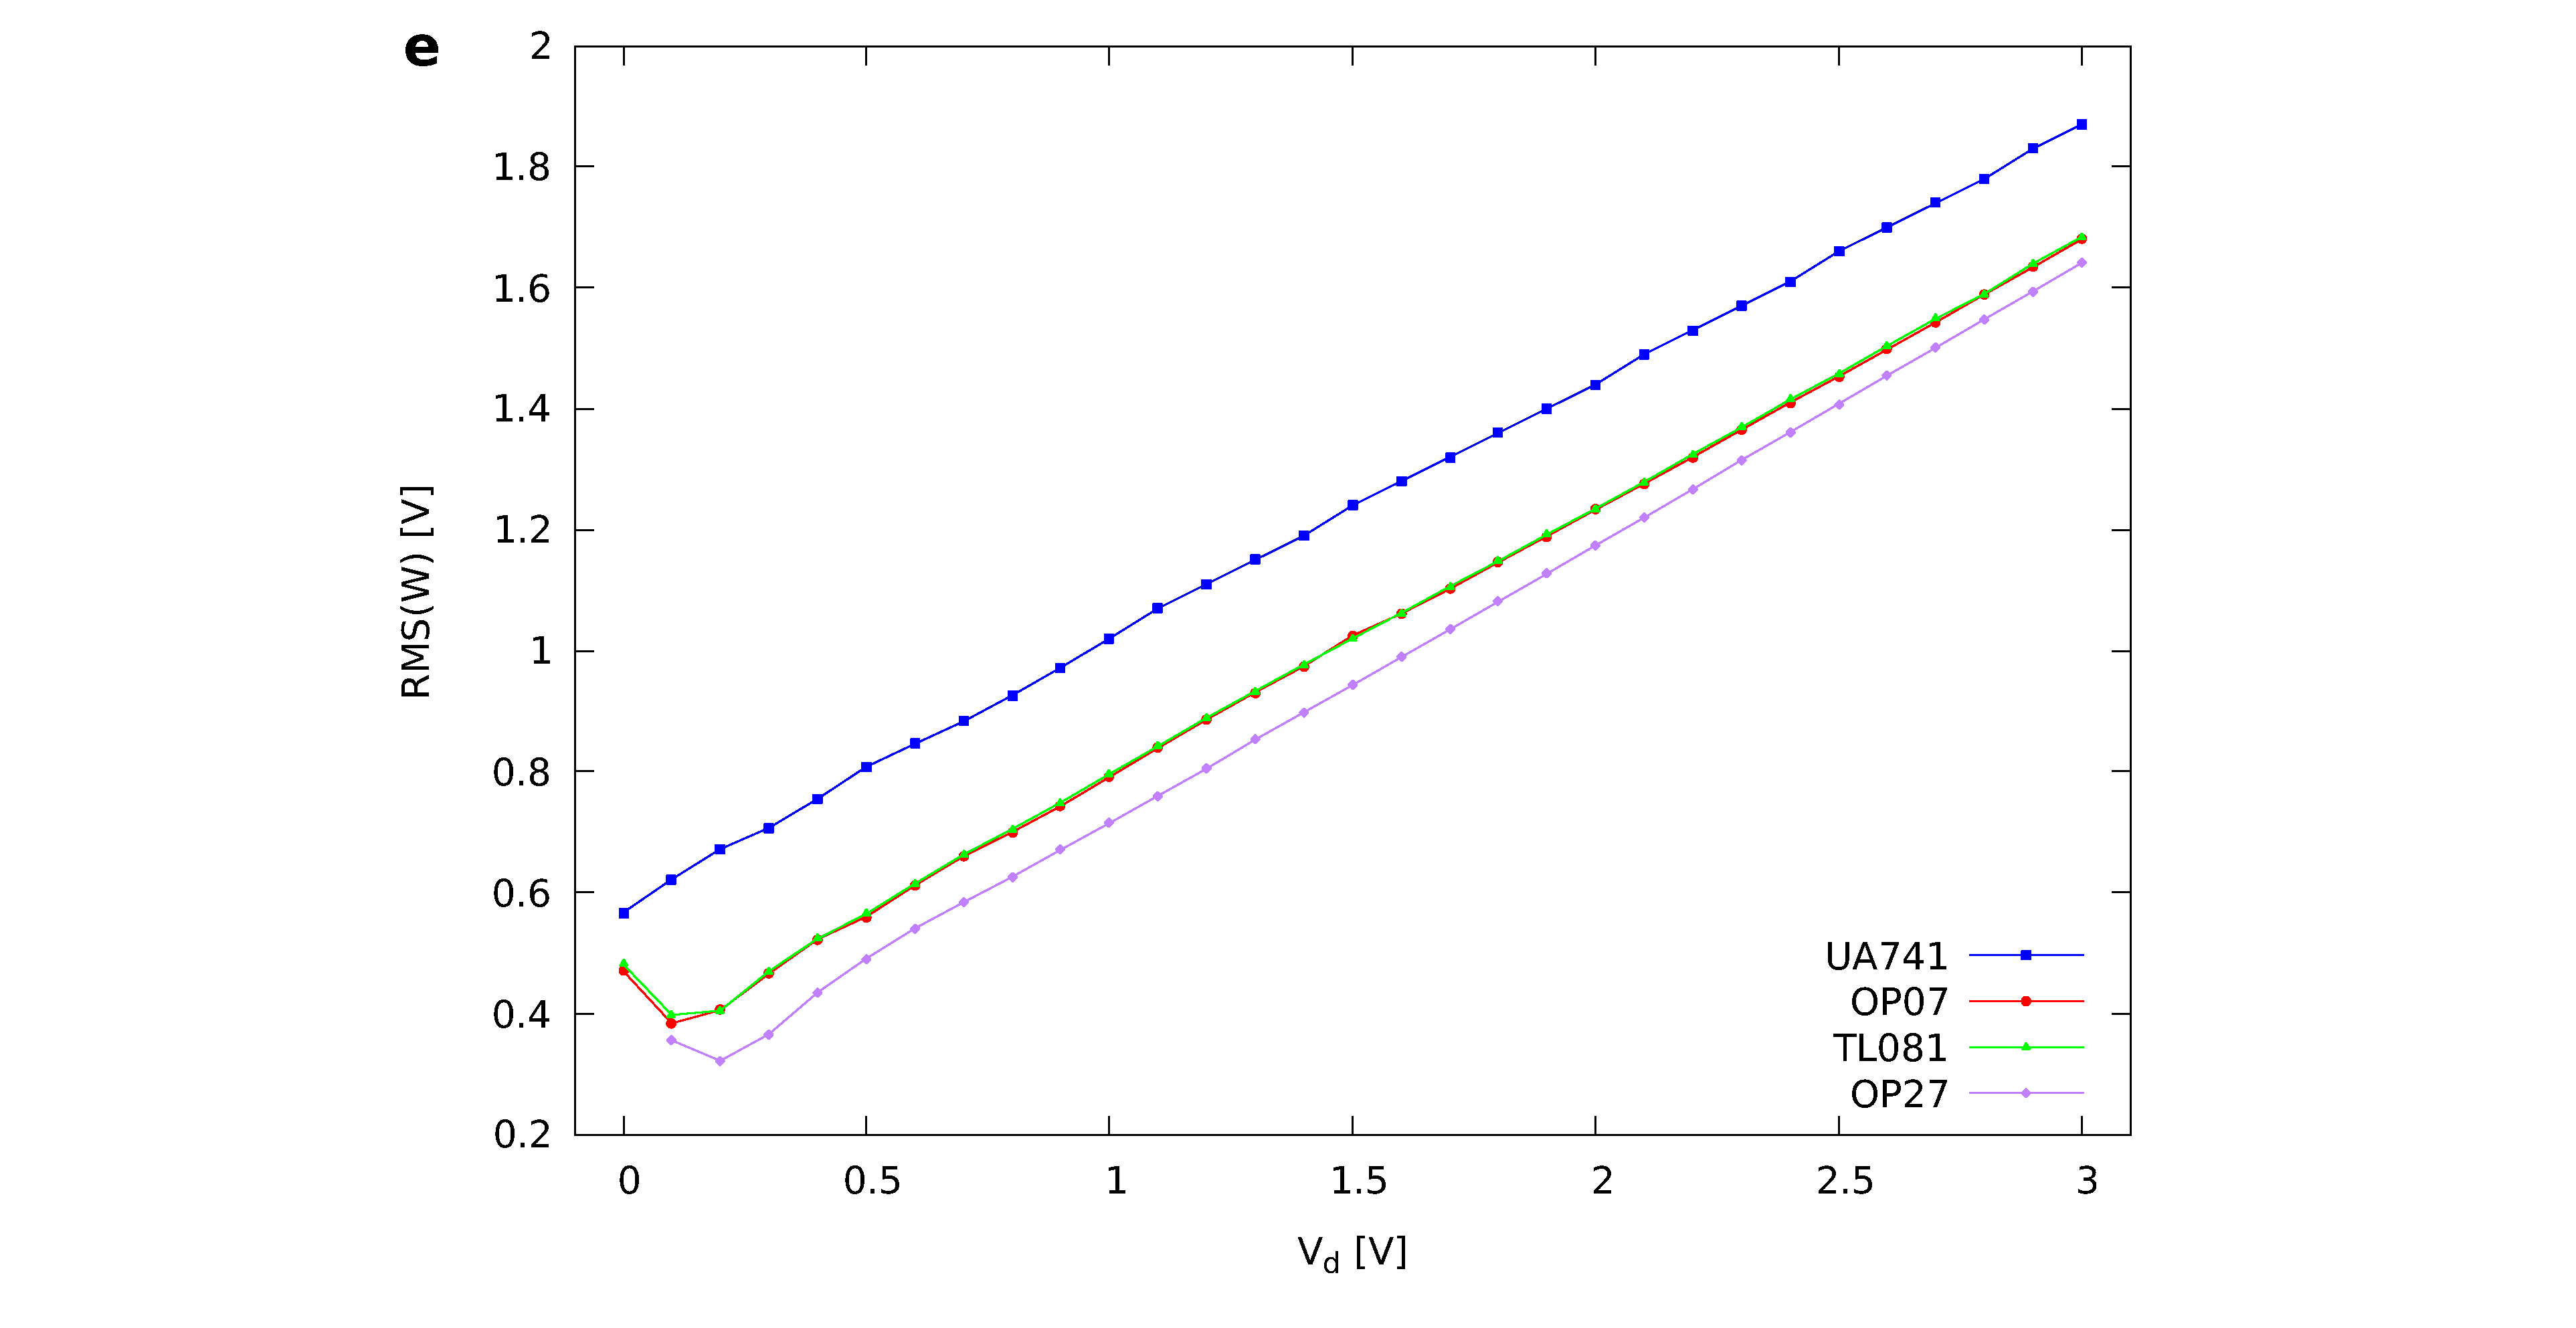
\includegraphics[width=\linewidth,trim={9cm 0 10cm 0},clip,right]
        {../1_block/breadboard/rms_bread.pdf}
    \end{subfigure}
    \caption{Oscillating behavior for the circuit implemented on
    the breadboard. (a) Plot of $W$ and (b) of $V$ as a function of time,
    for $V_d=1$ V.
    (c) Phase portrait (Lissajous figure) of $V$ versus $W$. (d)
    Frequency and (e) root mean square amplitude of the
    output signal $W$ as a function of the parameter $V_d$ and for
    different kinds of op-amps.}\label{fig:oscillation breadboard}
\end{figure}


\subsection{Prototypes}\label{sec:prototypes}

In order to describe the coupling between many oscillators it is
not possible use the breadboard implementation of the circuit
shown in Fig. \ref{fig:breadboard implementation}, due to
scalability issues. For the purpose of improving the system
scalability, two smaller prototypical chips have been built.
The circuit implemented in each chip is shown in Fig.
\ref{fig:prototype implementation}. The differences between this
circuit and the one used in the previous subsection lie in the nonlinear
elements; in this case MBRA210L Schottky diodes have been used,
as well as quad operational amplifiers OP470, which offer
comparable performance to OP27 op-amps.

The oscillating behavior of this circuit is shown in Fig.
\ref{fig:oscillation prototype} for both chips. These systems are much
less stable with respect to the circuit implemented on the breadboard;
in fact, measurements were possible only in a small range for $V_d$,
namely $V_d \leq 1.1$ V for one chip and $V_d \leq 0.6$ V for the
other one. It is also important to point out that the diode clamping
is not present; in fact, it is only noticeable at voltages
$V_d \lesssim 0.4$ V.


\begin{figure}[H]
    \centering
    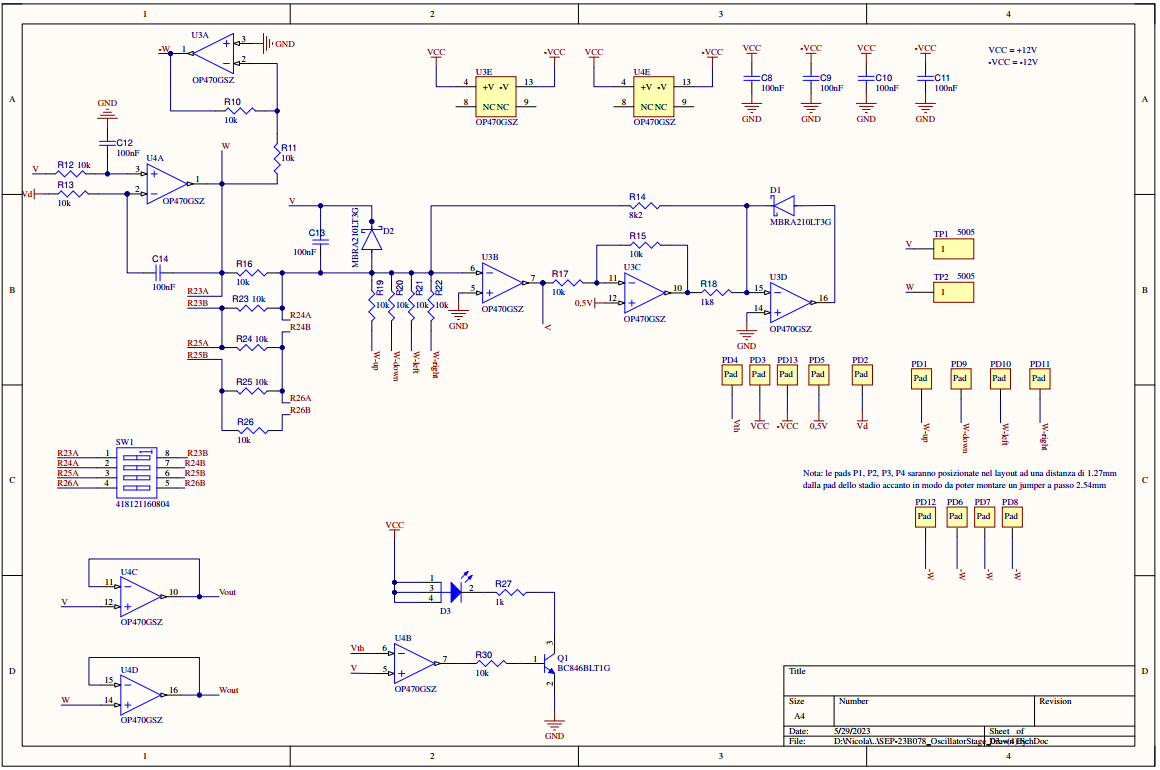
\includegraphics[width=0.75\linewidth]
    {../1_block/prototypes/prototype_implementation.png}
    \caption{Circuit diagram of one prototypical chip.}
    \label{fig:prototype implementation}
\end{figure}

\begin{figure}[H]
    \centering
    \begin{minipage}{.58\textwidth}
        \begin{subfigure}{\linewidth}
            \centering
            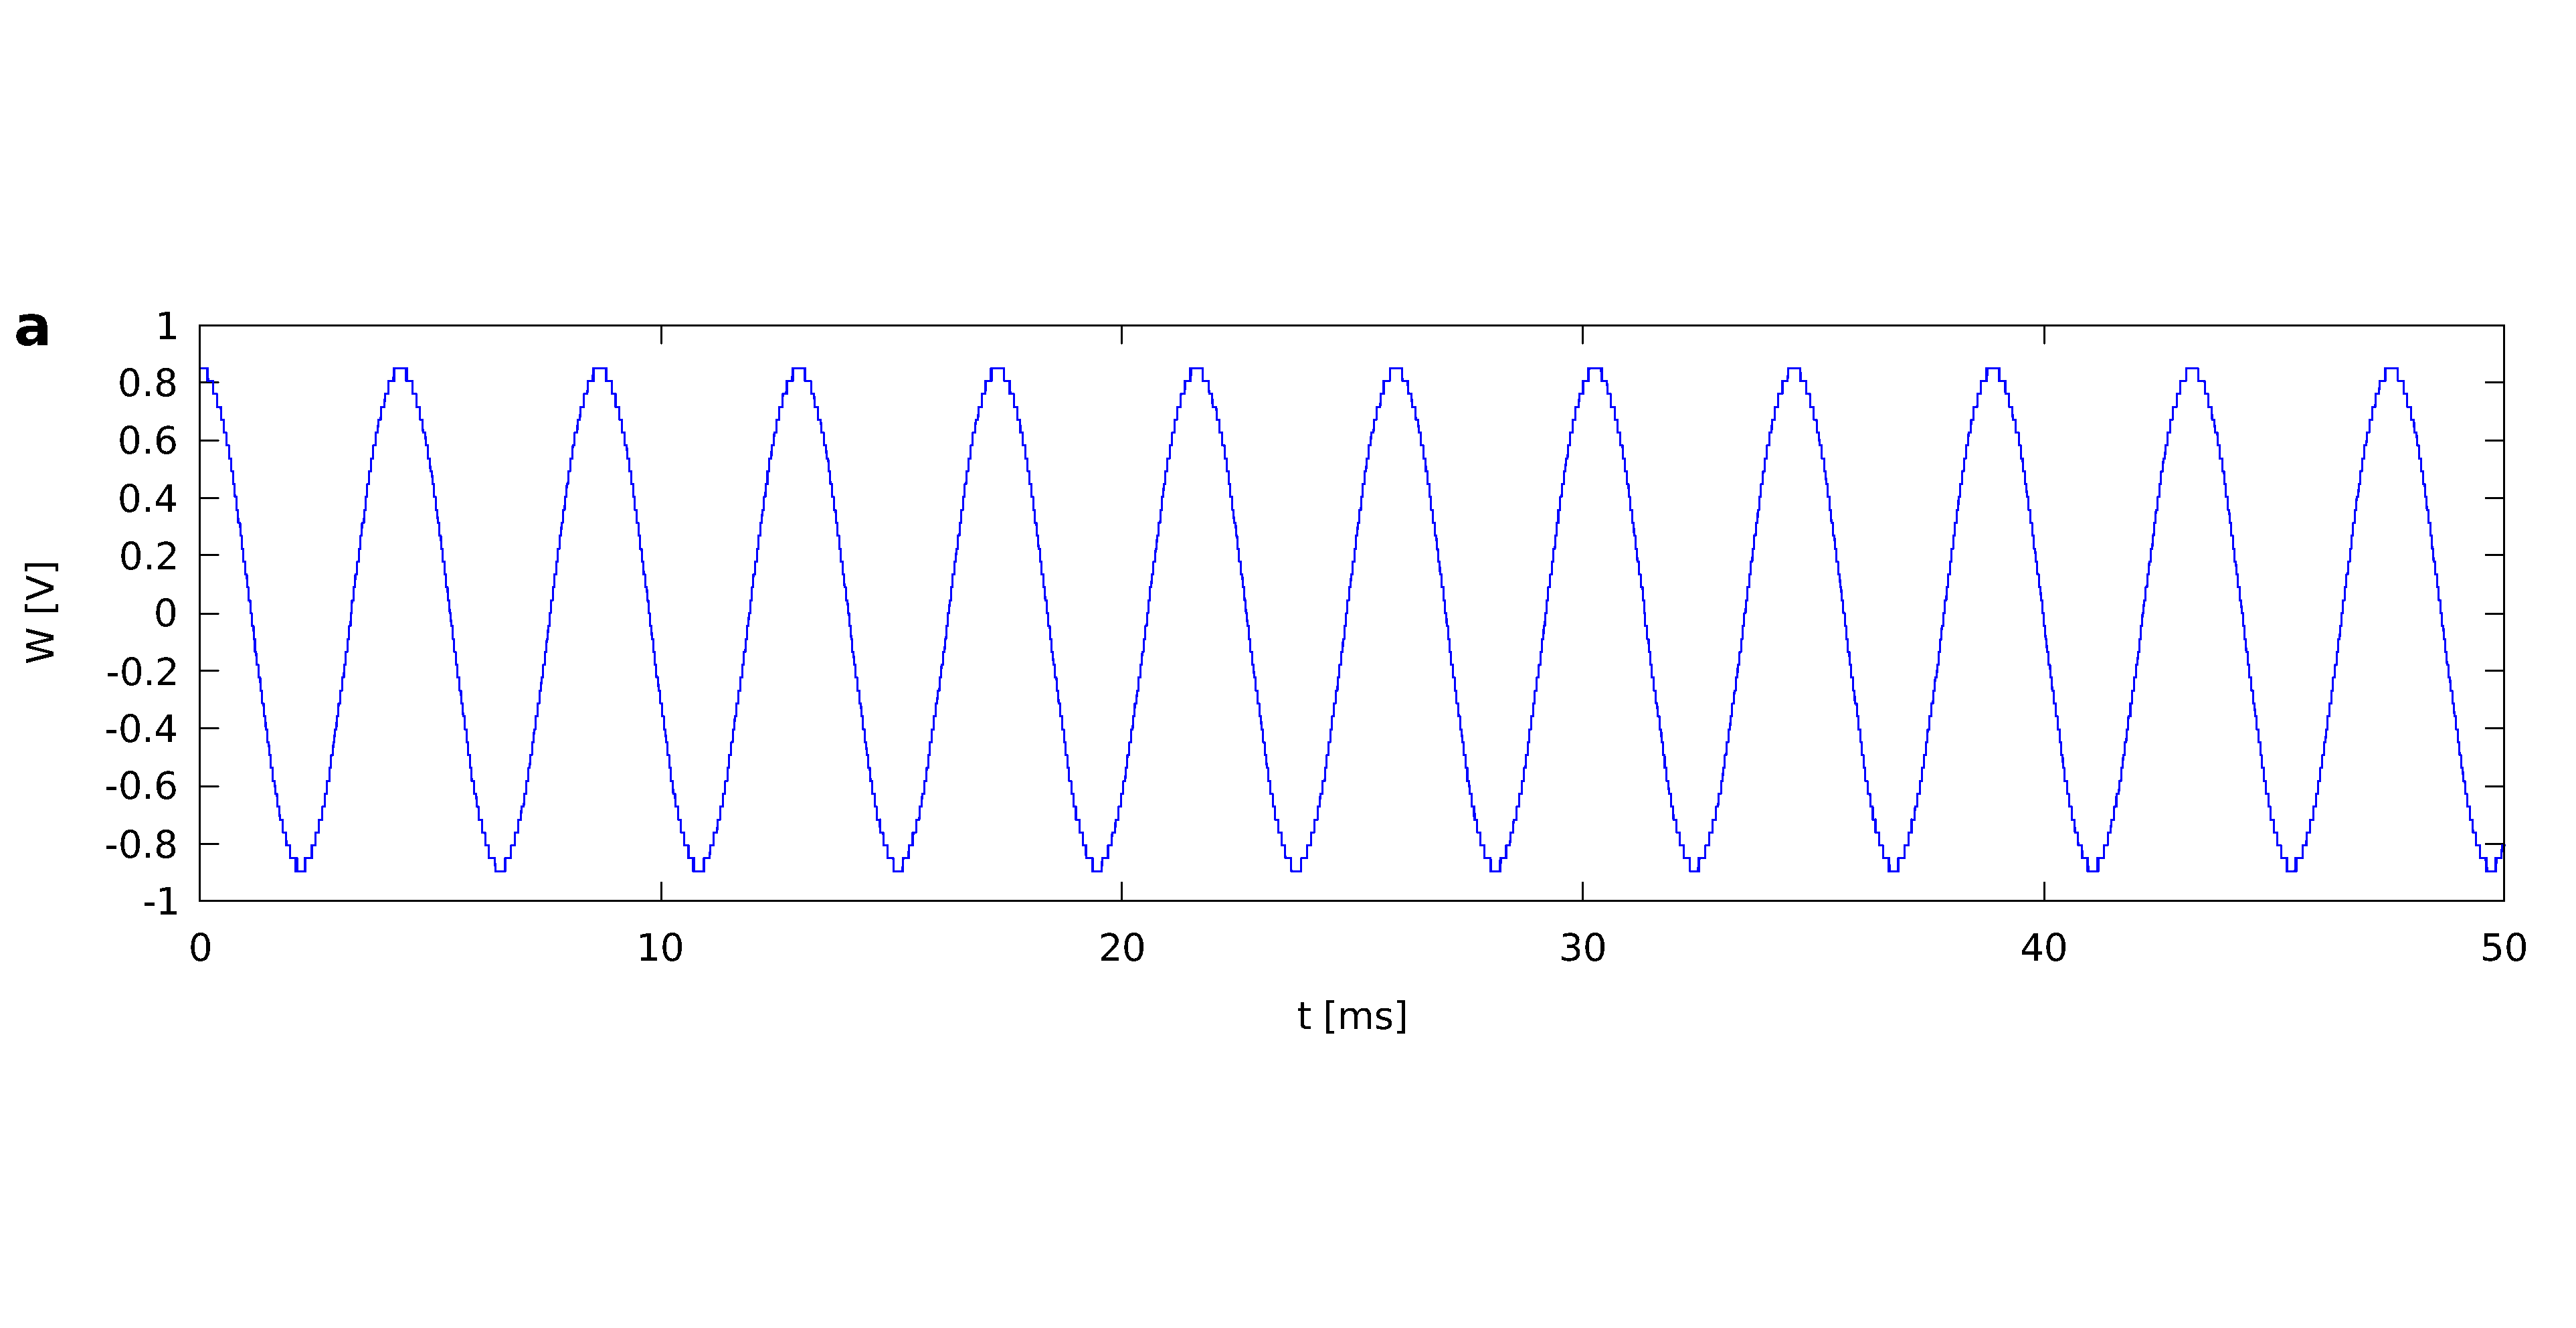
\includegraphics[width=\linewidth,trim={0 6cm 0 6cm},clip,left]
            {../1_block/prototypes/W_wf.pdf}\\
            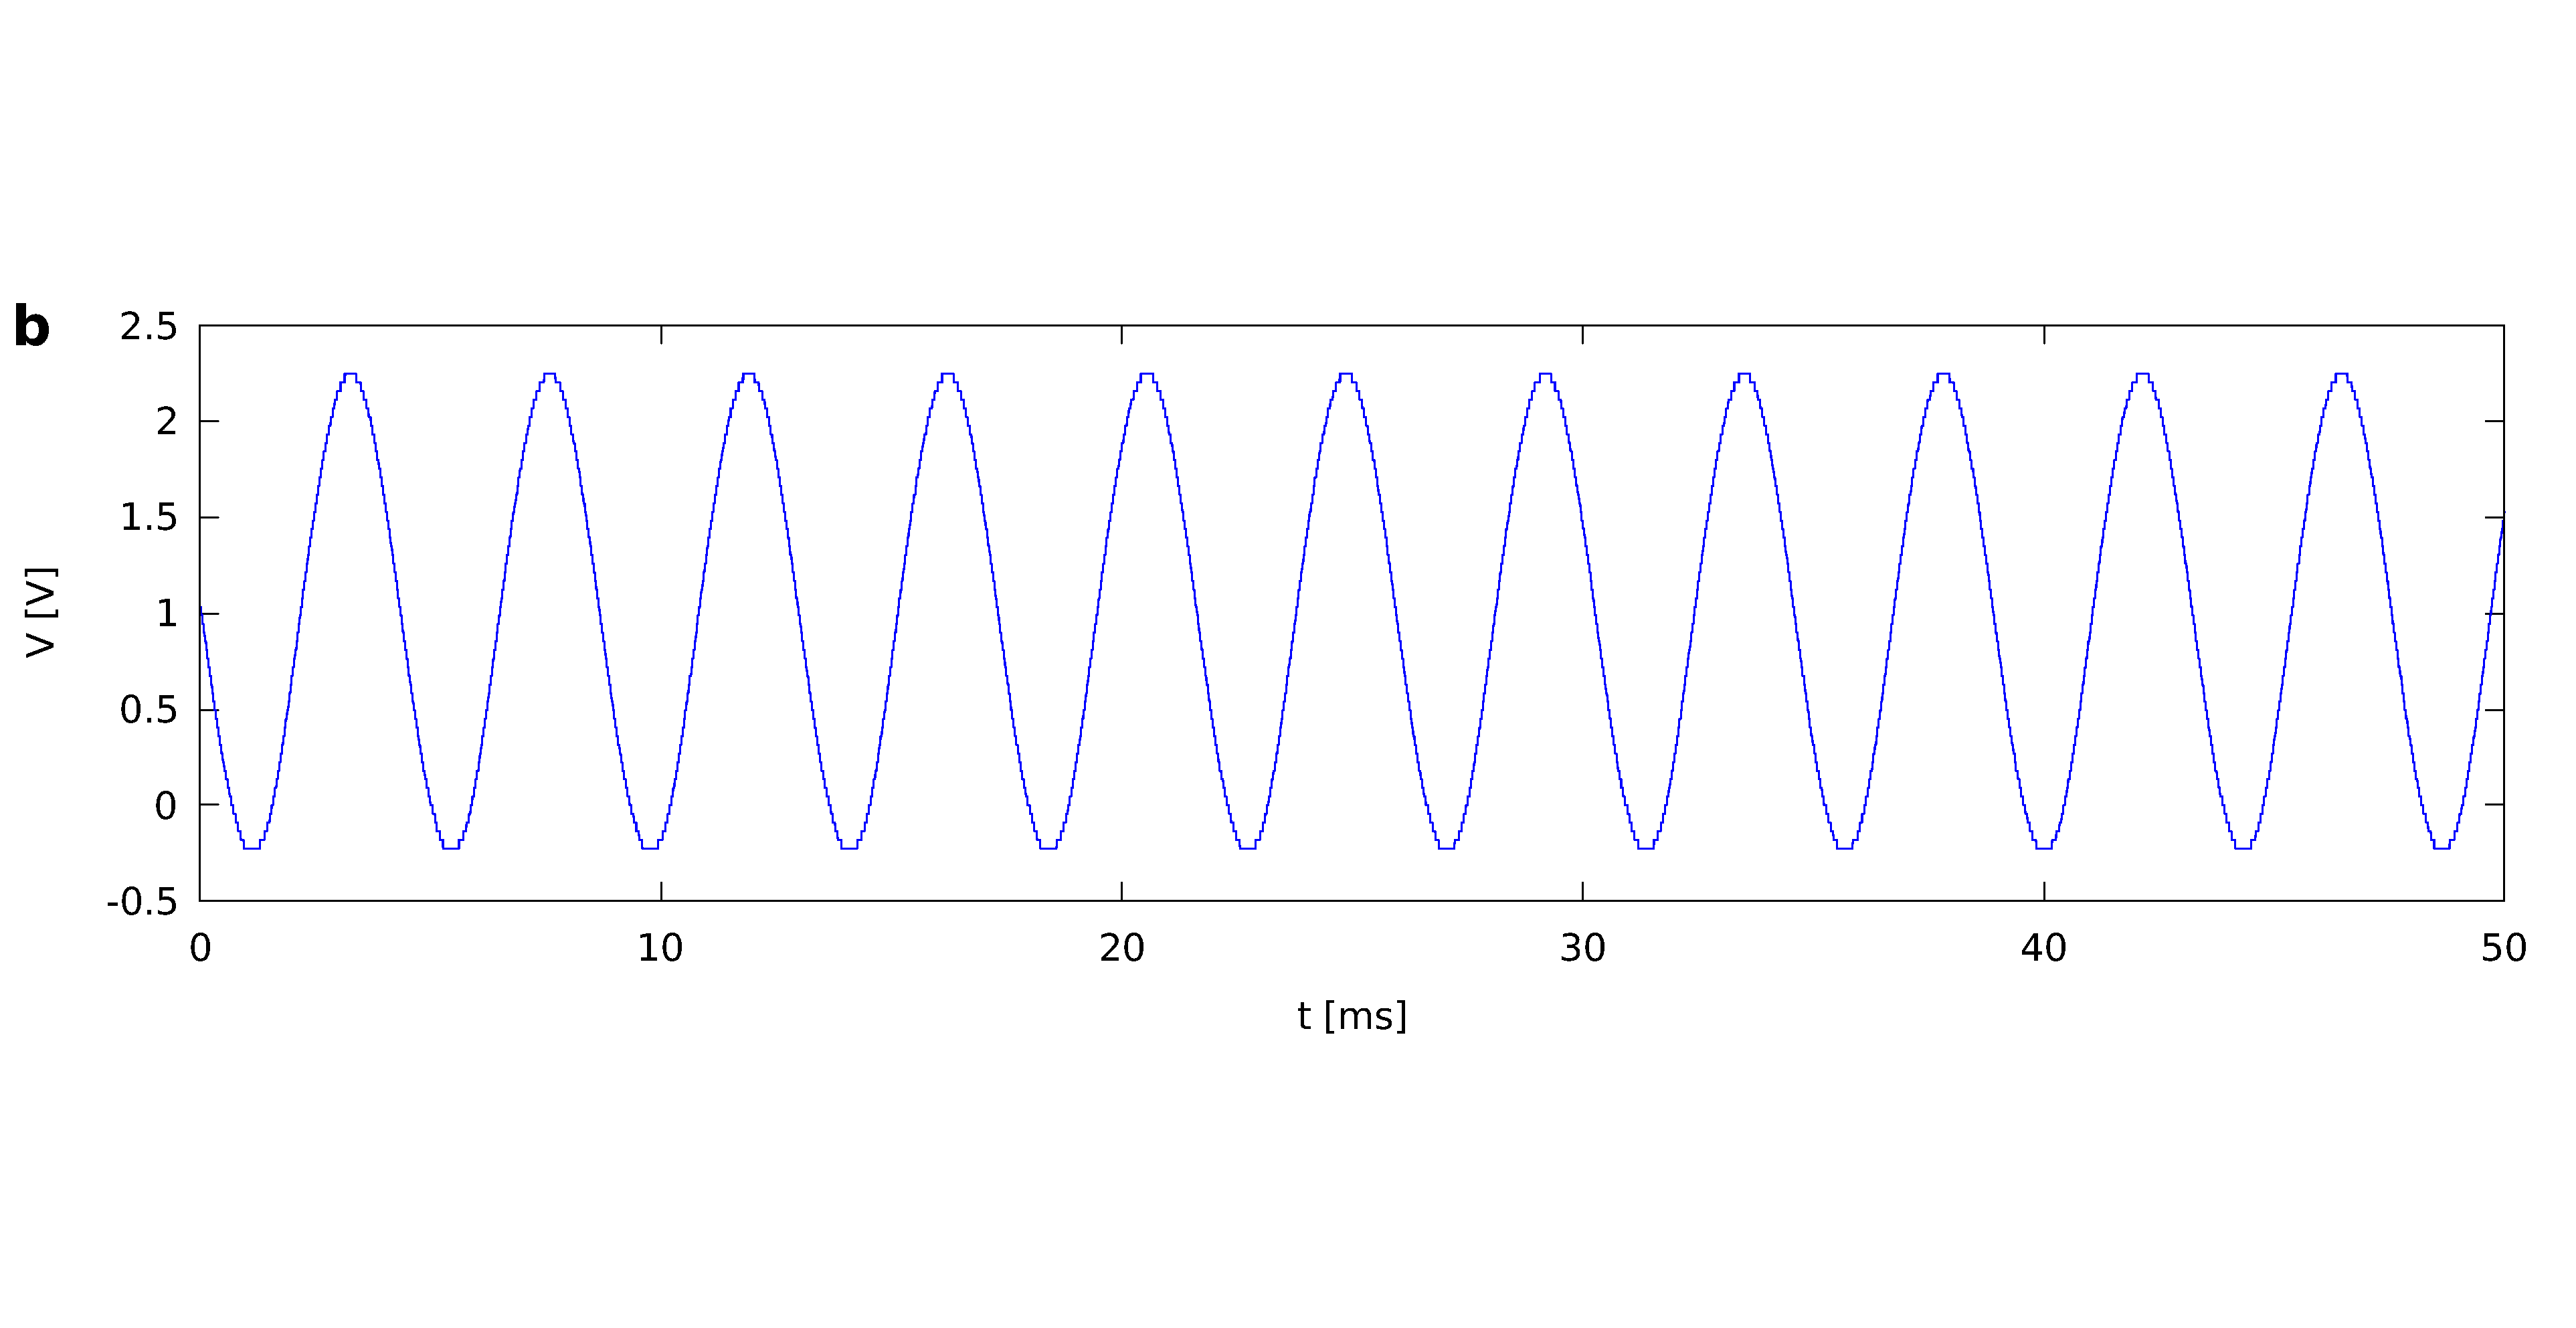
\includegraphics[width=\linewidth,trim={0 6cm 0 6cm},clip,left]
            {../1_block/prototypes/V_wf.pdf}
        \end{subfigure}
    \end{minipage}
    \begin{subfigure}{.39\textwidth}
        \centering
        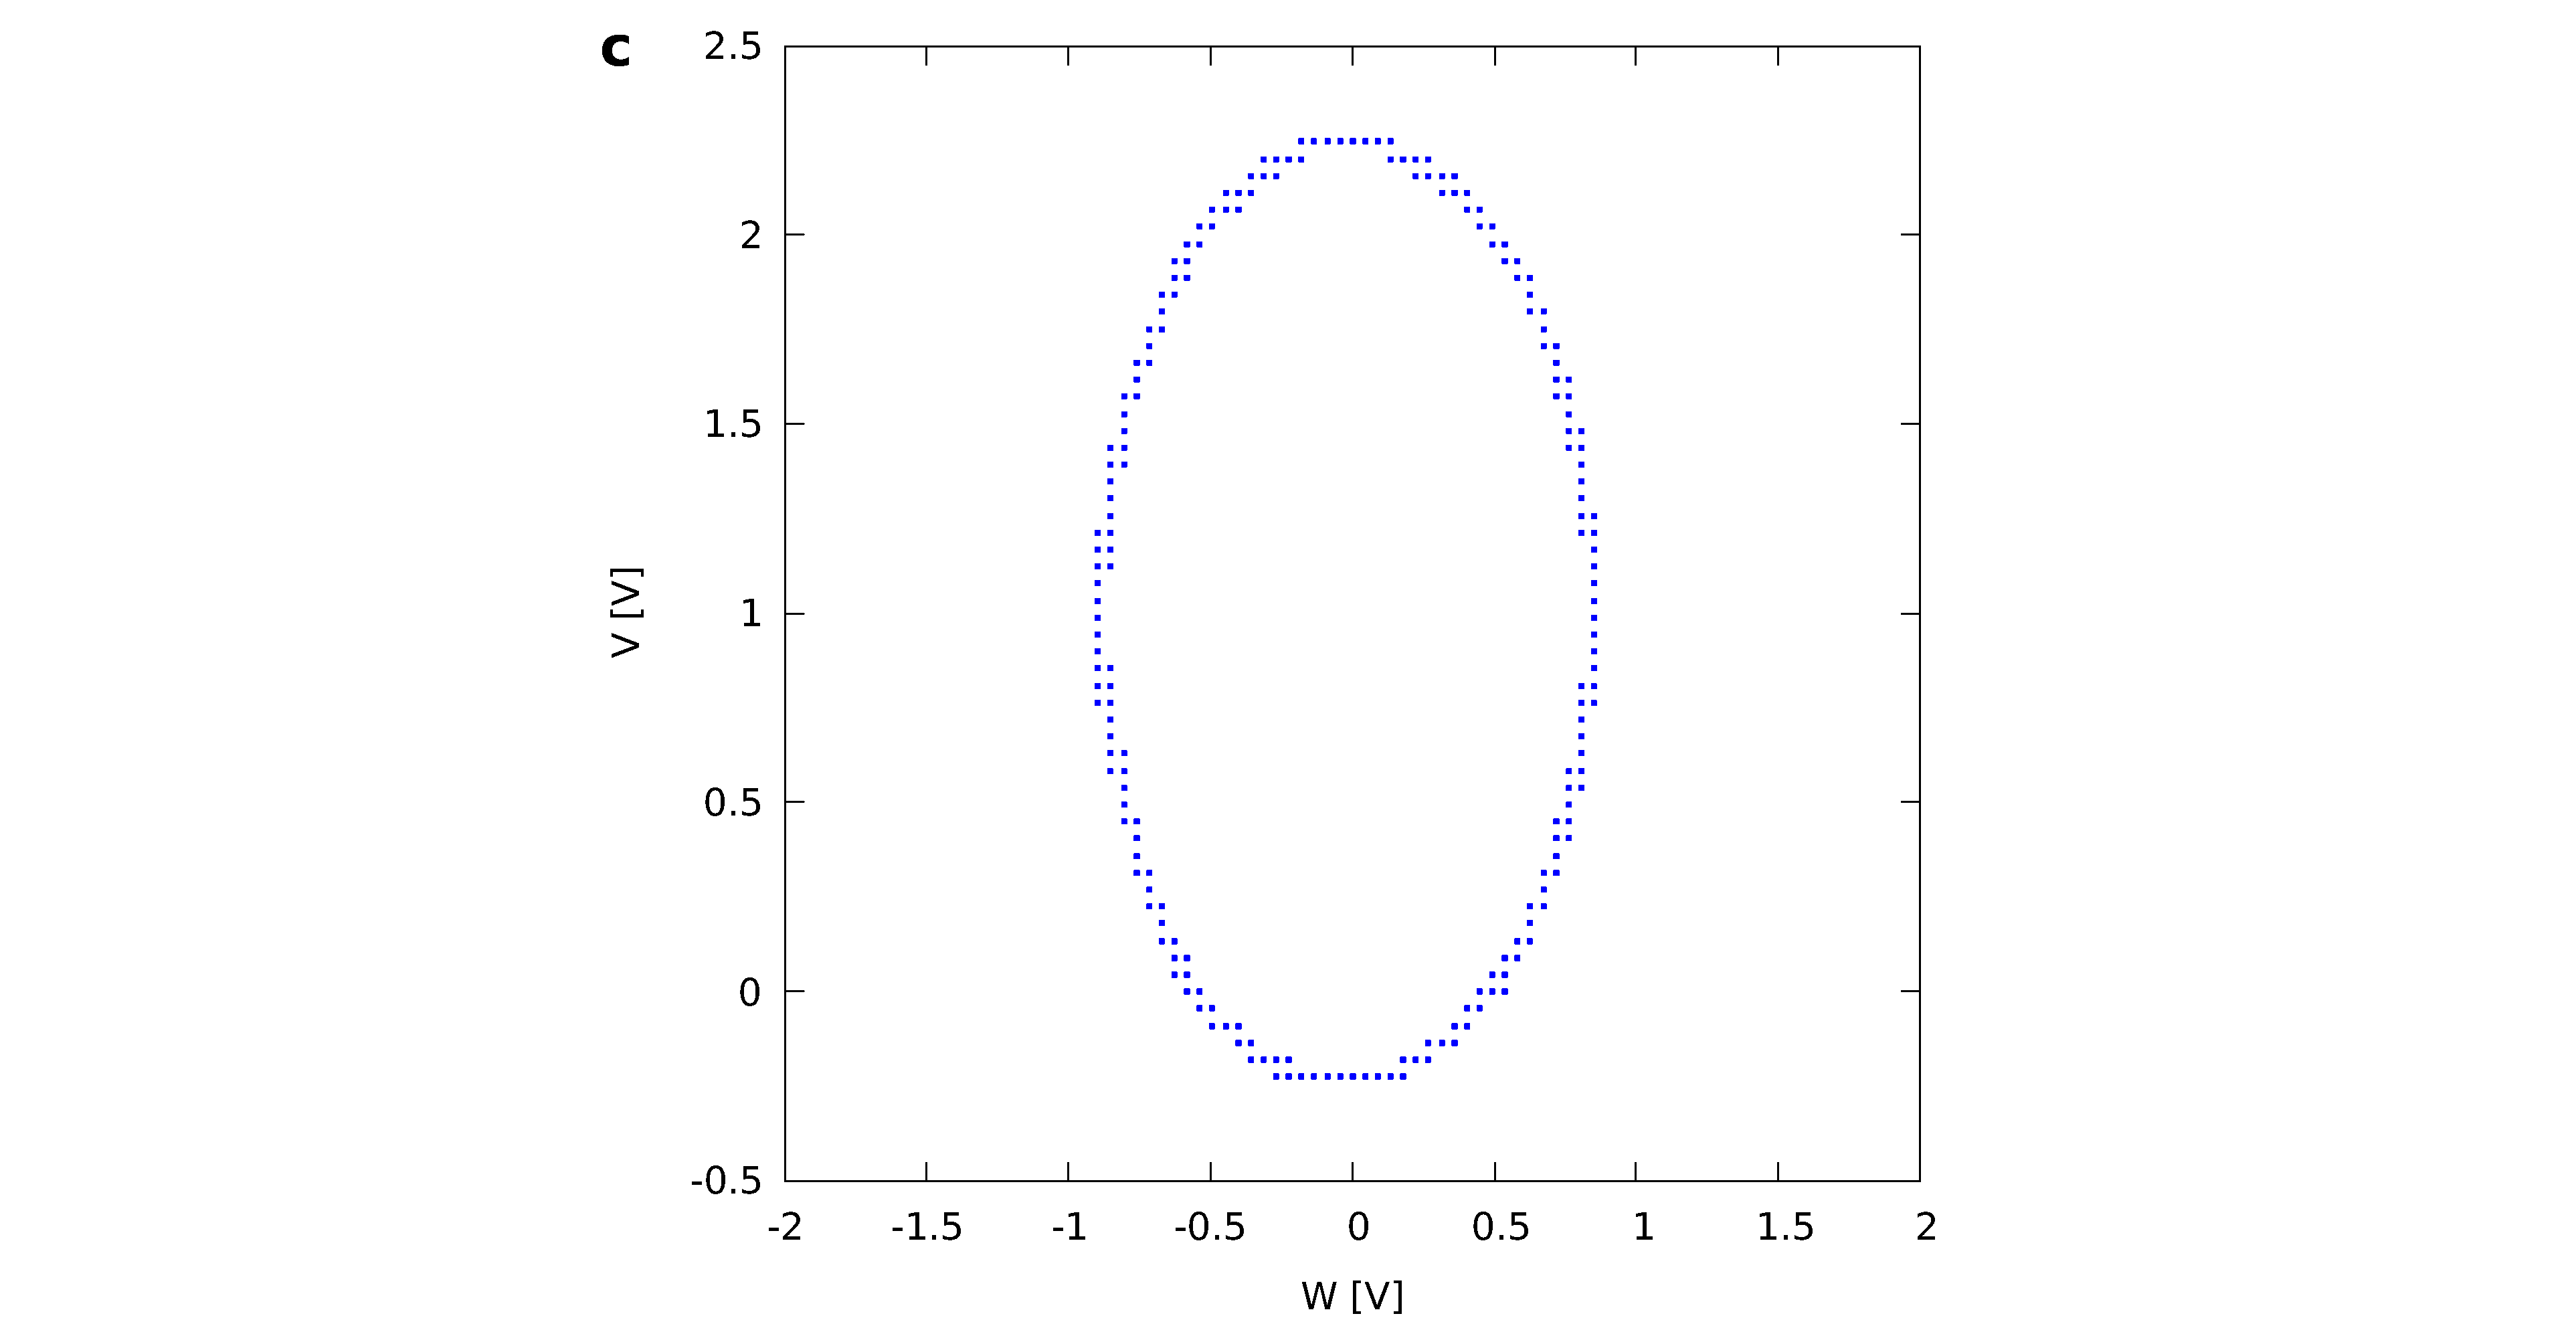
\includegraphics[width=\linewidth,trim={15cm 0 15cm 0},clip,right]
        {../1_block/prototypes/Lissajous.pdf}
    \end{subfigure}
    \begin{subfigure}{.49\textwidth}
        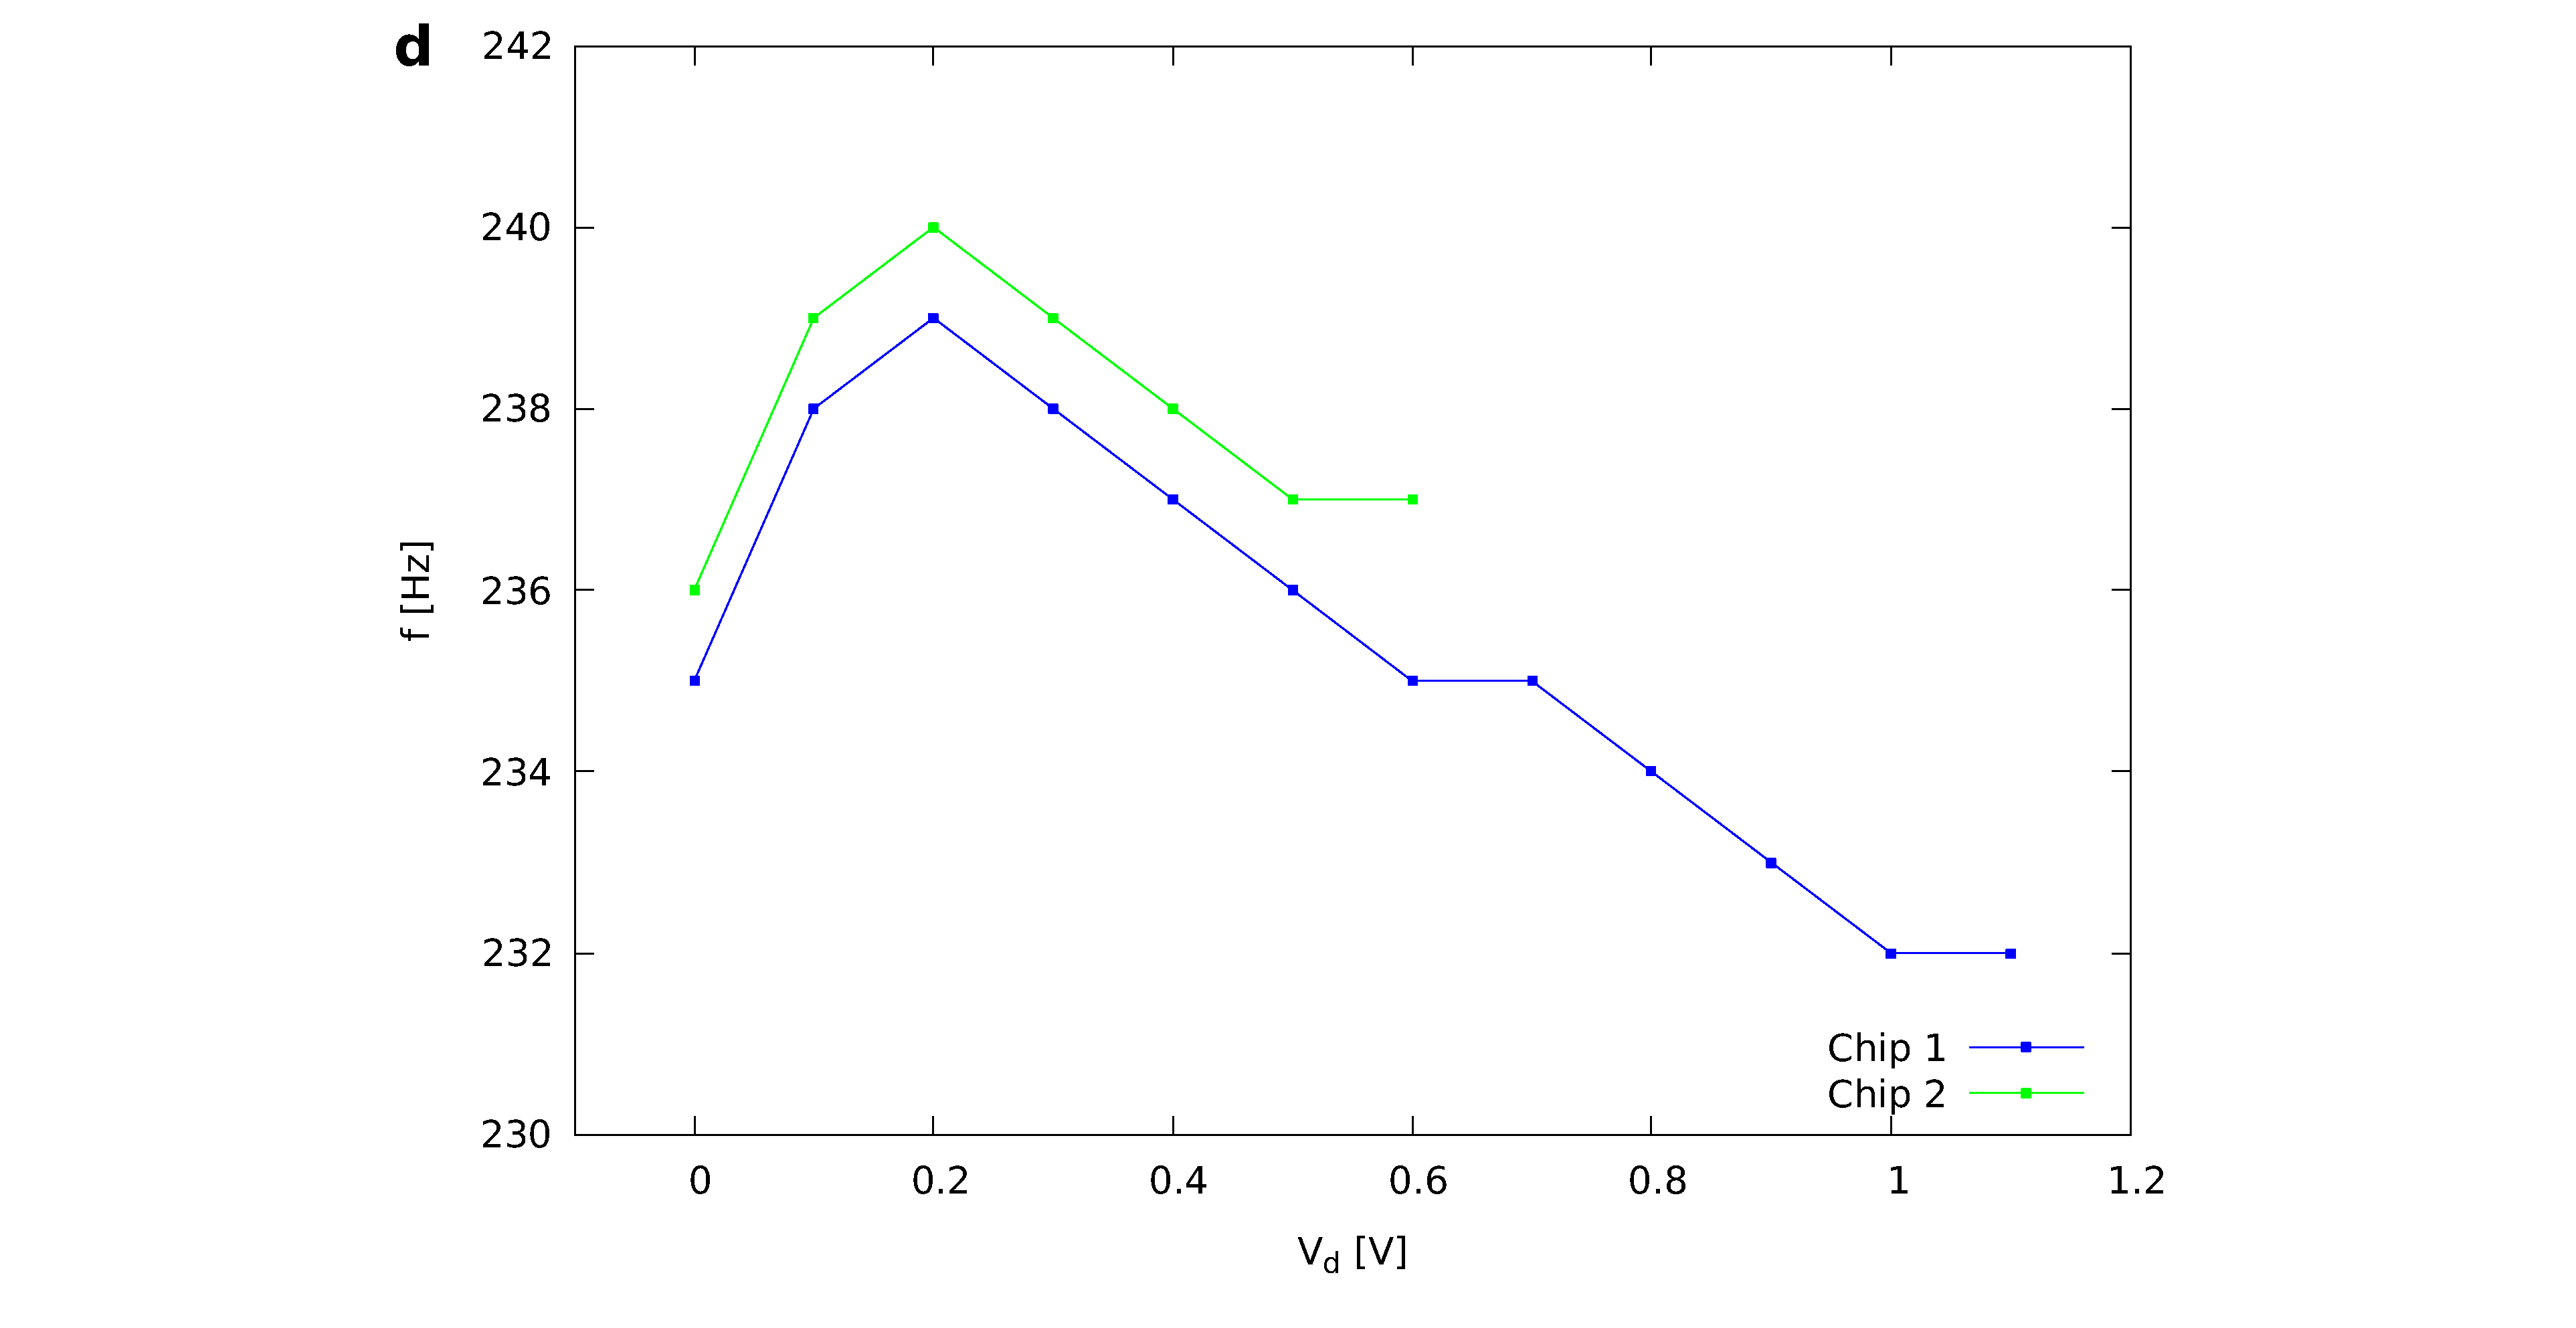
\includegraphics[width=\linewidth,trim={10cm 0 9cm 0},clip,left]
        {../1_block/prototypes/freq_prot.pdf}
    \end{subfigure}
    \begin{subfigure}{.49\textwidth}
        \centering
        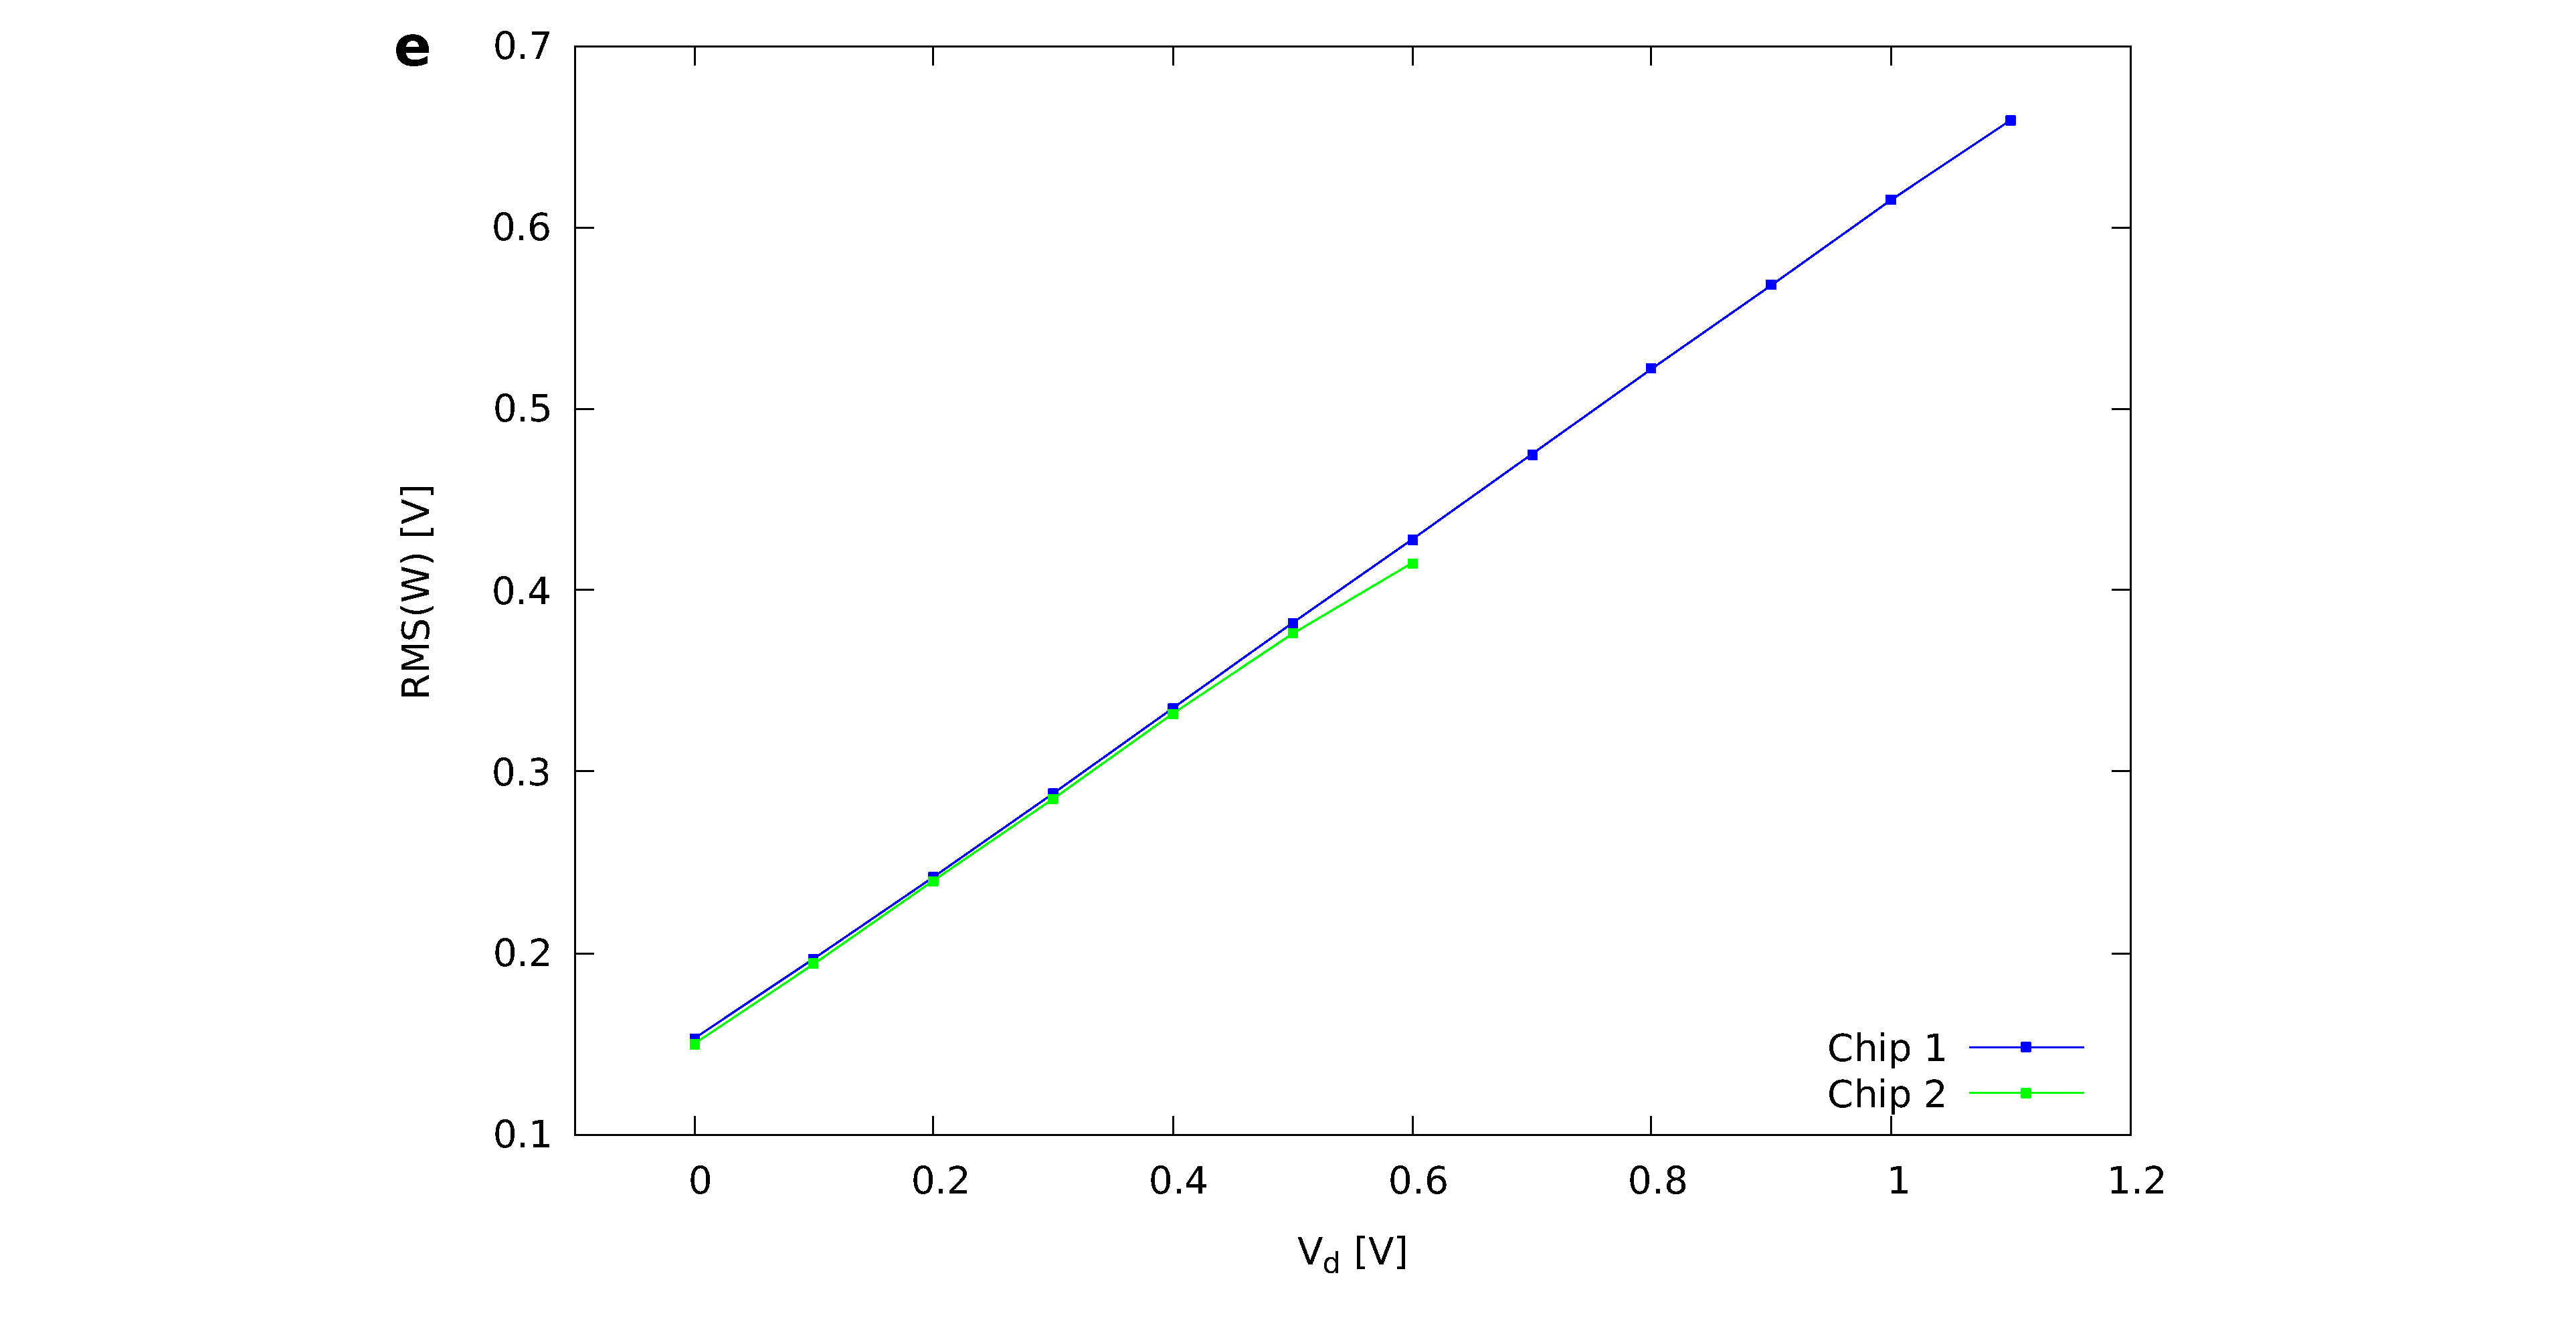
\includegraphics[width=\linewidth,trim={9cm 0 10cm 0},clip,right]
        {../1_block/prototypes/rms_prot.pdf}
    \end{subfigure}
    \caption{Oscillating behavior for the circuit implemented on
    the prototypical chips. (a) Plot of $W$ and (b) of $V$ as a
    function of time, for $V_d=1$ V.
    (c) Phase portrait (Lissajous figure) of $V$ versus $W$. (d)
    Frequency and (e) root mean square amplitude of the
    output signal $W$ as a function of the parameter $V_d$ and for
    the two different chips.}
    \label{fig:oscillation prototype}
\end{figure}

\subsection{Board}\label{sec:board}

In order to finally analyze the behavior of many coupled
oscillators, a board containing 25 chips (or blocks) has been built.
The circuit diagram is equivalent to the one shown in Fig.
\ref{fig:prototype implementation} for the prototypes, the only
difference being the use of DFLS1100 Schottky diodes instead of
MBRA210L ones.

The oscillating behavior is shown in Fig.
\ref{fig:oscillation board}. Once again, these systems are not as
stable as the circuit on the breadboard; measurements were in fact
taken for $V_d \leq 2.2$ V for the first two blocks. It is important to notice
that in the voltage range $0.6~\text{V} \leq V_d \leq 2.1~\text{V}$
a clamping of the output voltage $V$ can be observed; this is not
intended and is probably due to intrinsic limitations in the current.

\begin{figure}[H]
    \centering
    \begin{minipage}{.58\textwidth}
        \begin{subfigure}{\linewidth}
            \centering
            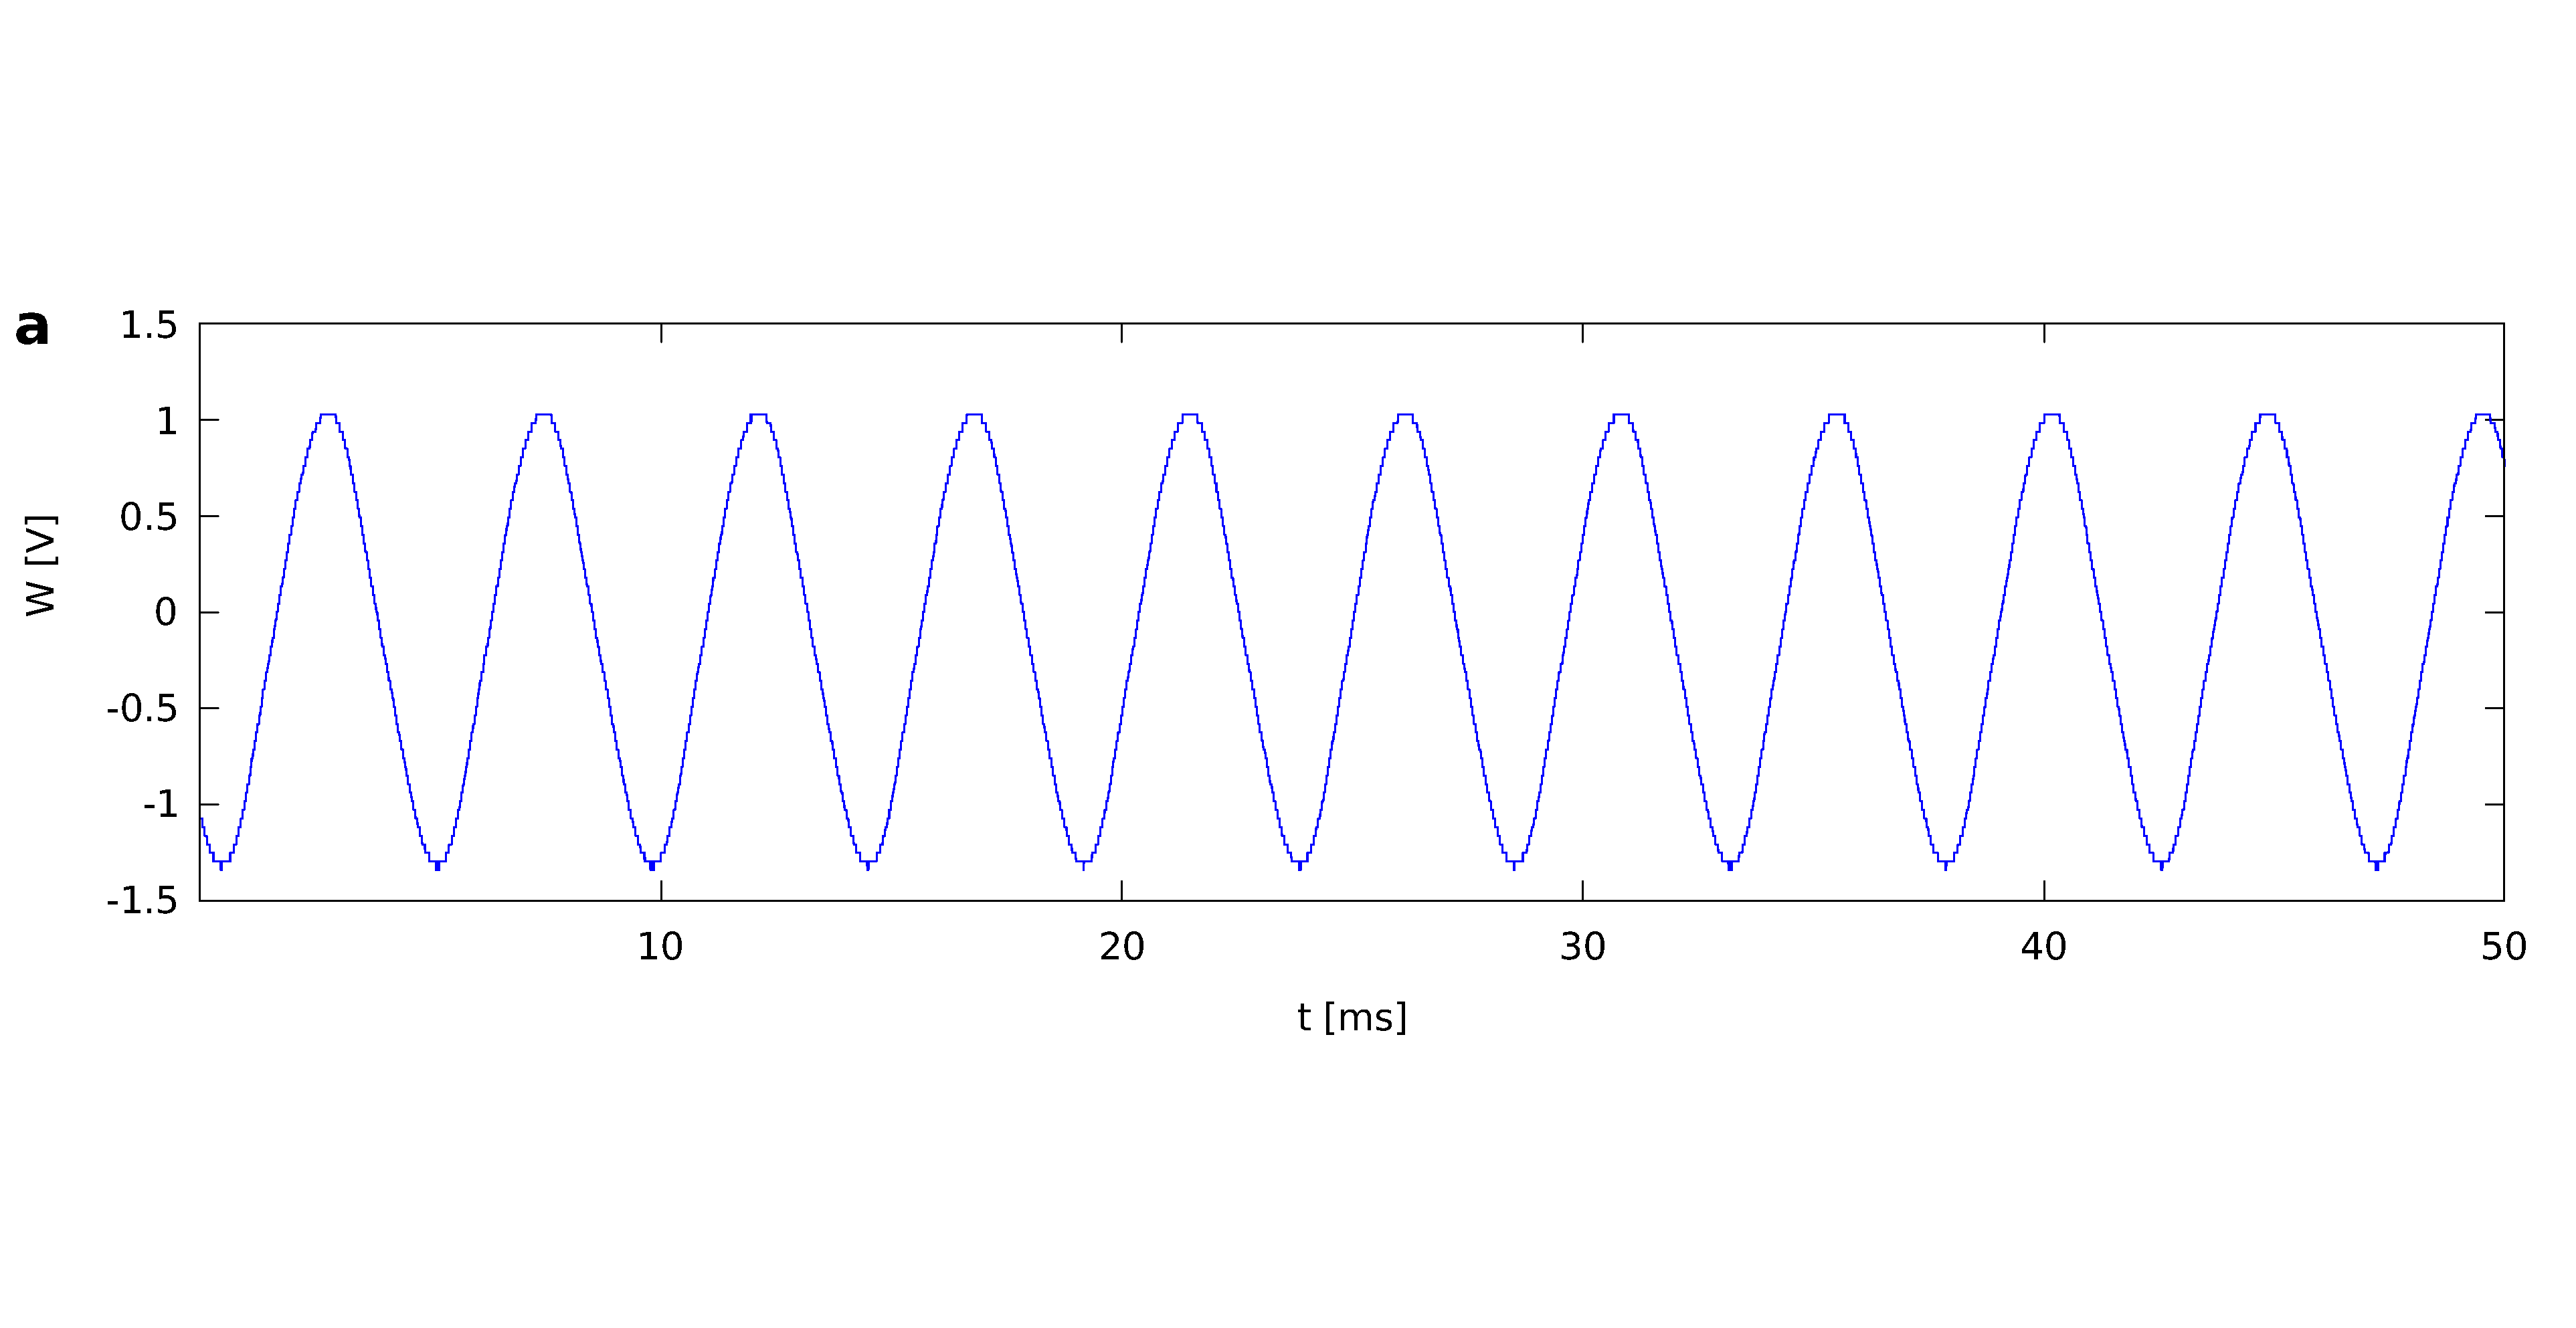
\includegraphics[width=\linewidth,trim={0 6cm 0 6cm},clip,left]
            {../1_block/board/W_wf.pdf}\\
            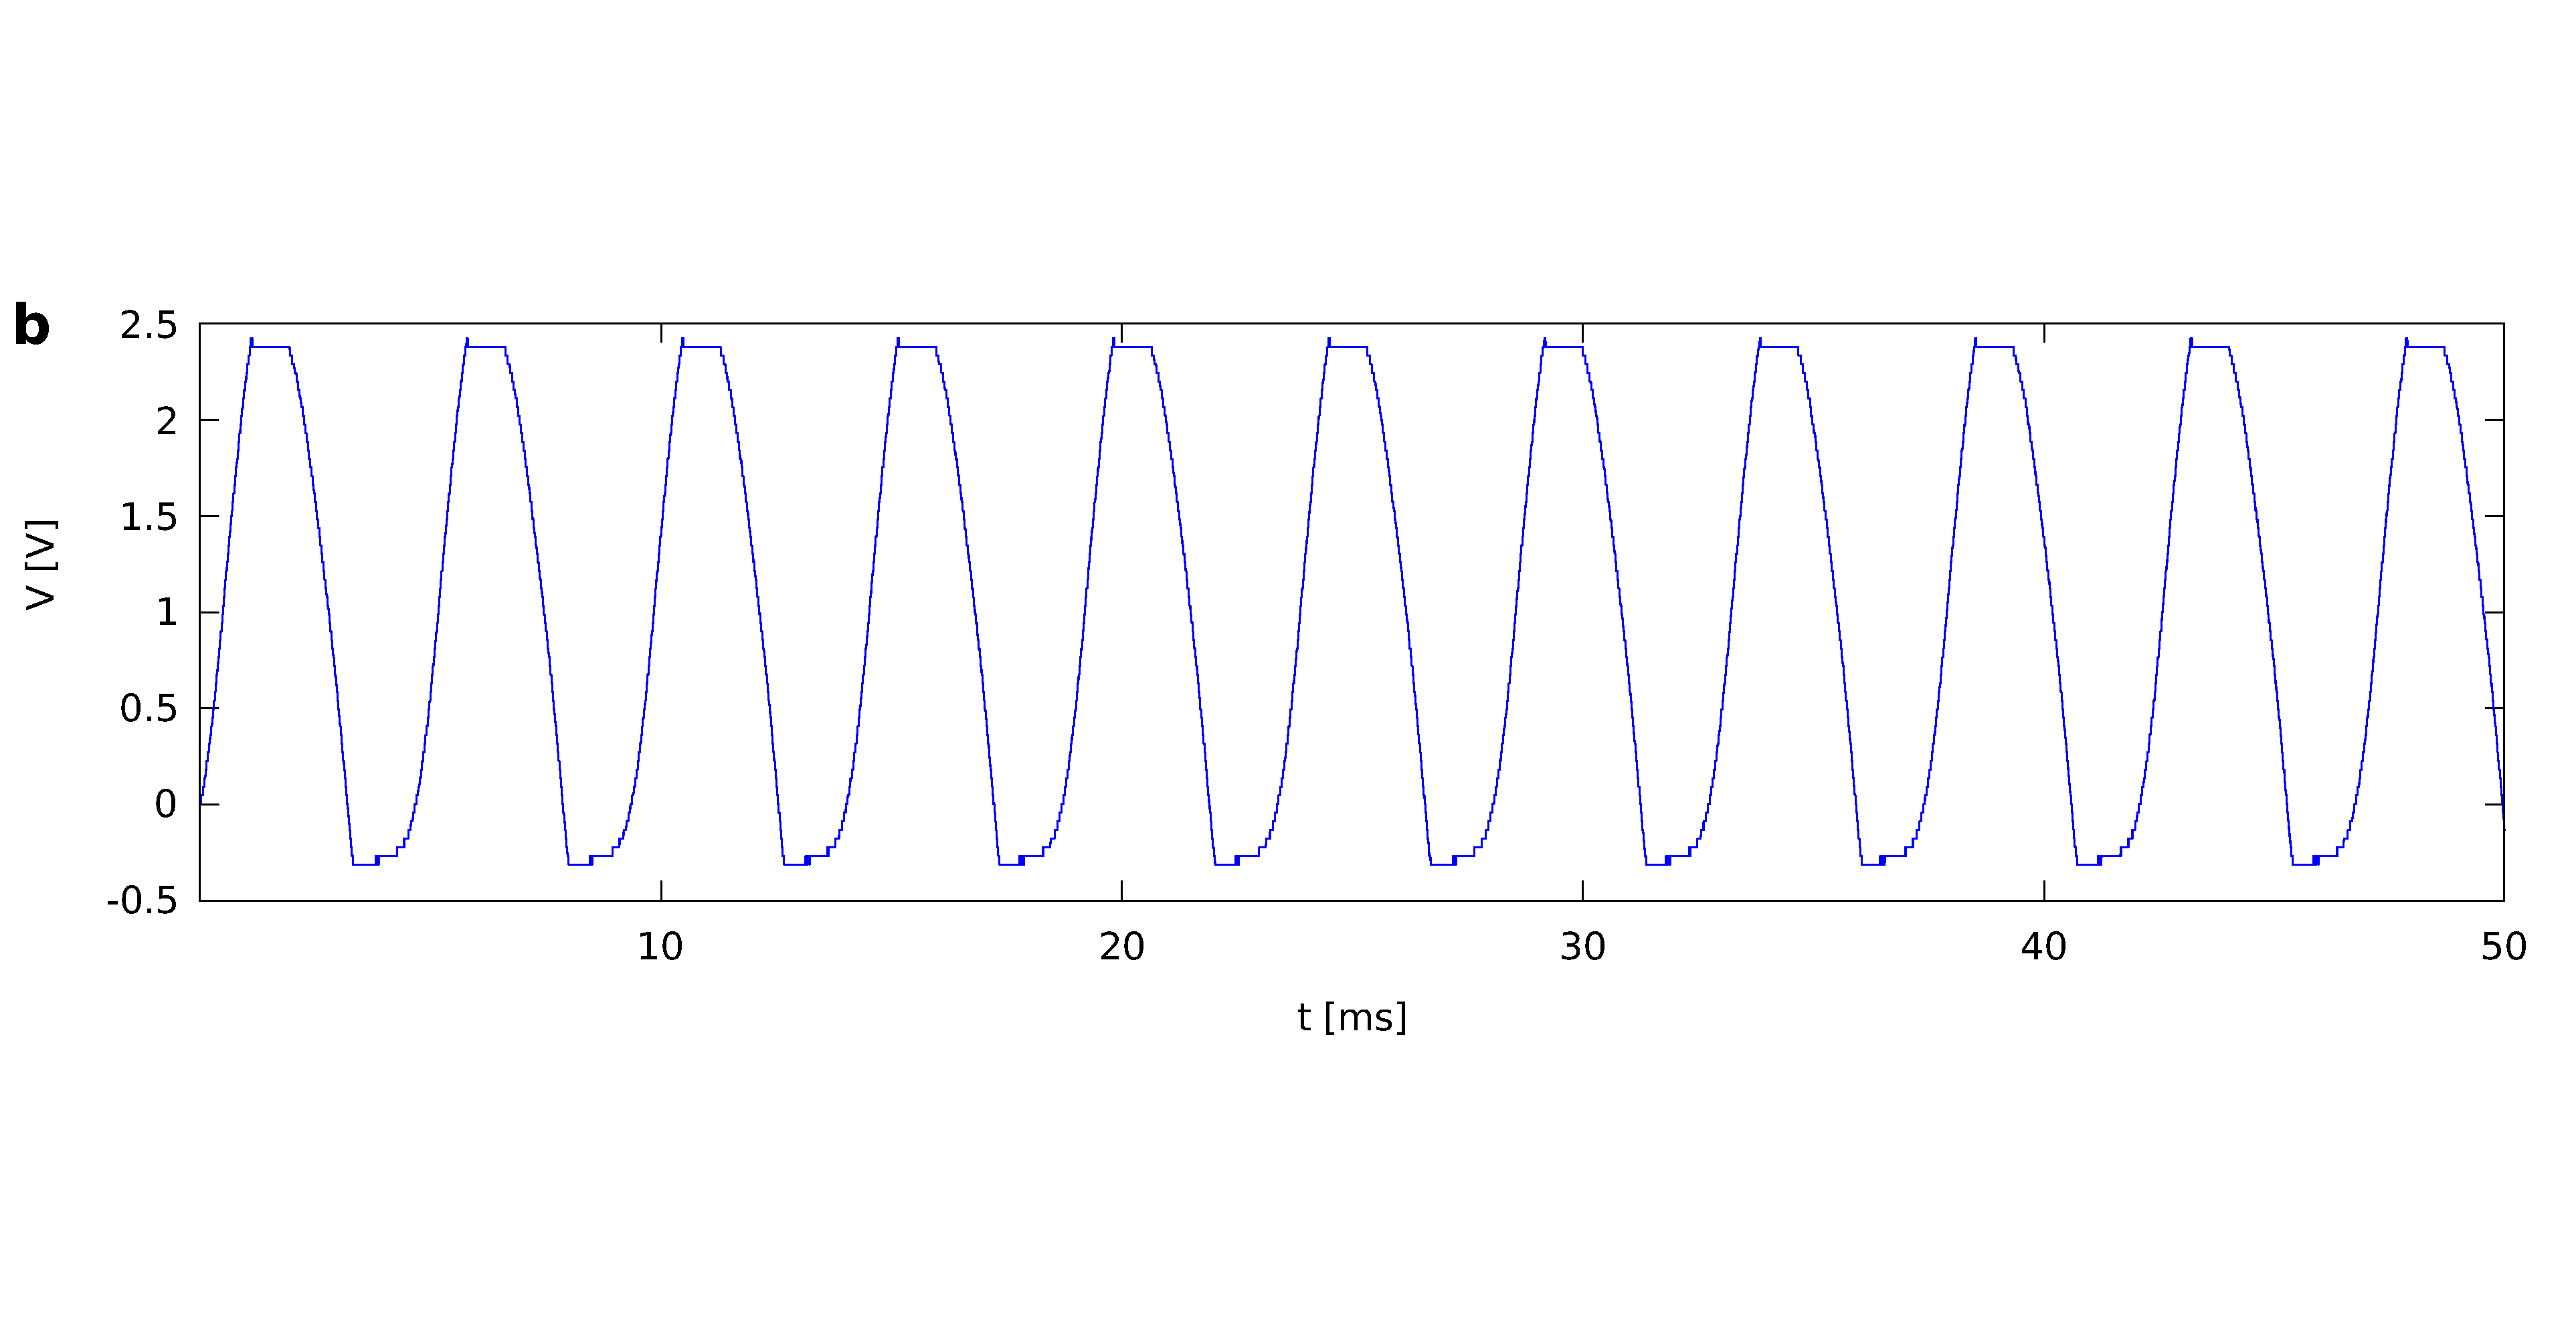
\includegraphics[width=\linewidth,trim={0 6cm 0 6cm},clip,left]
            {../1_block/board/V_wf.pdf}
        \end{subfigure}
    \end{minipage}
    \begin{subfigure}{.39\textwidth}
        \centering
        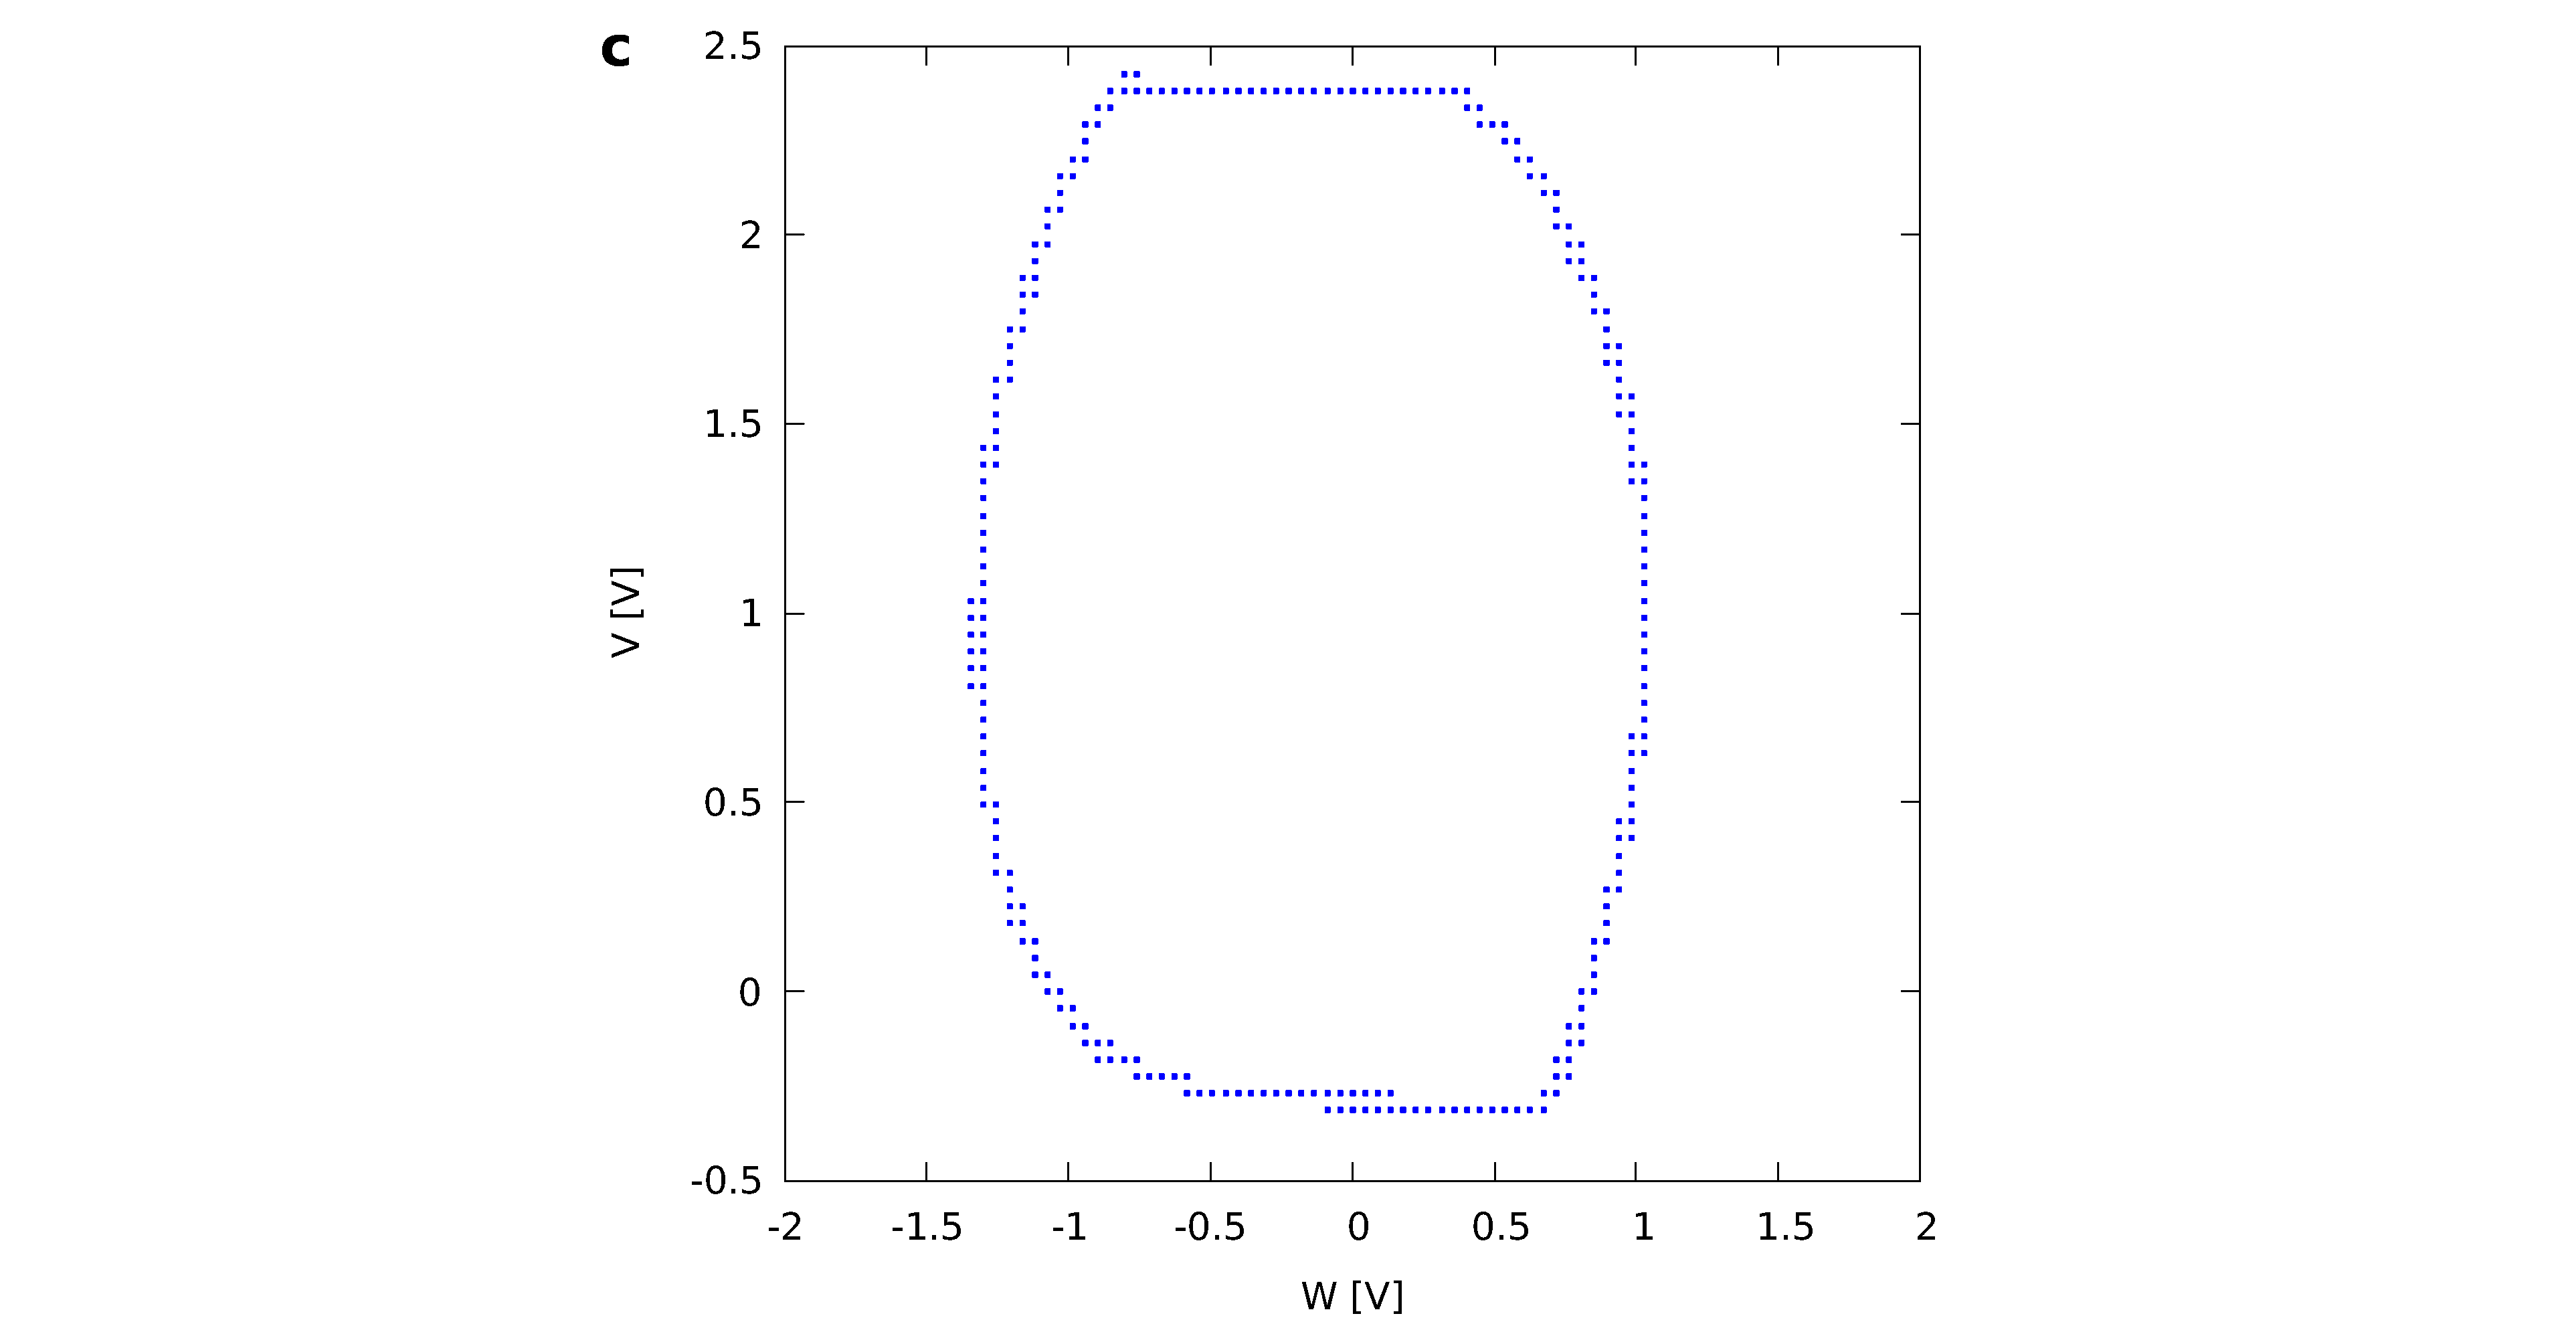
\includegraphics[width=\linewidth,trim={15cm 0 15cm 0},clip,right]
        {../1_block/board/Lissajous.pdf}
    \end{subfigure}
    \begin{subfigure}{.49\textwidth}
        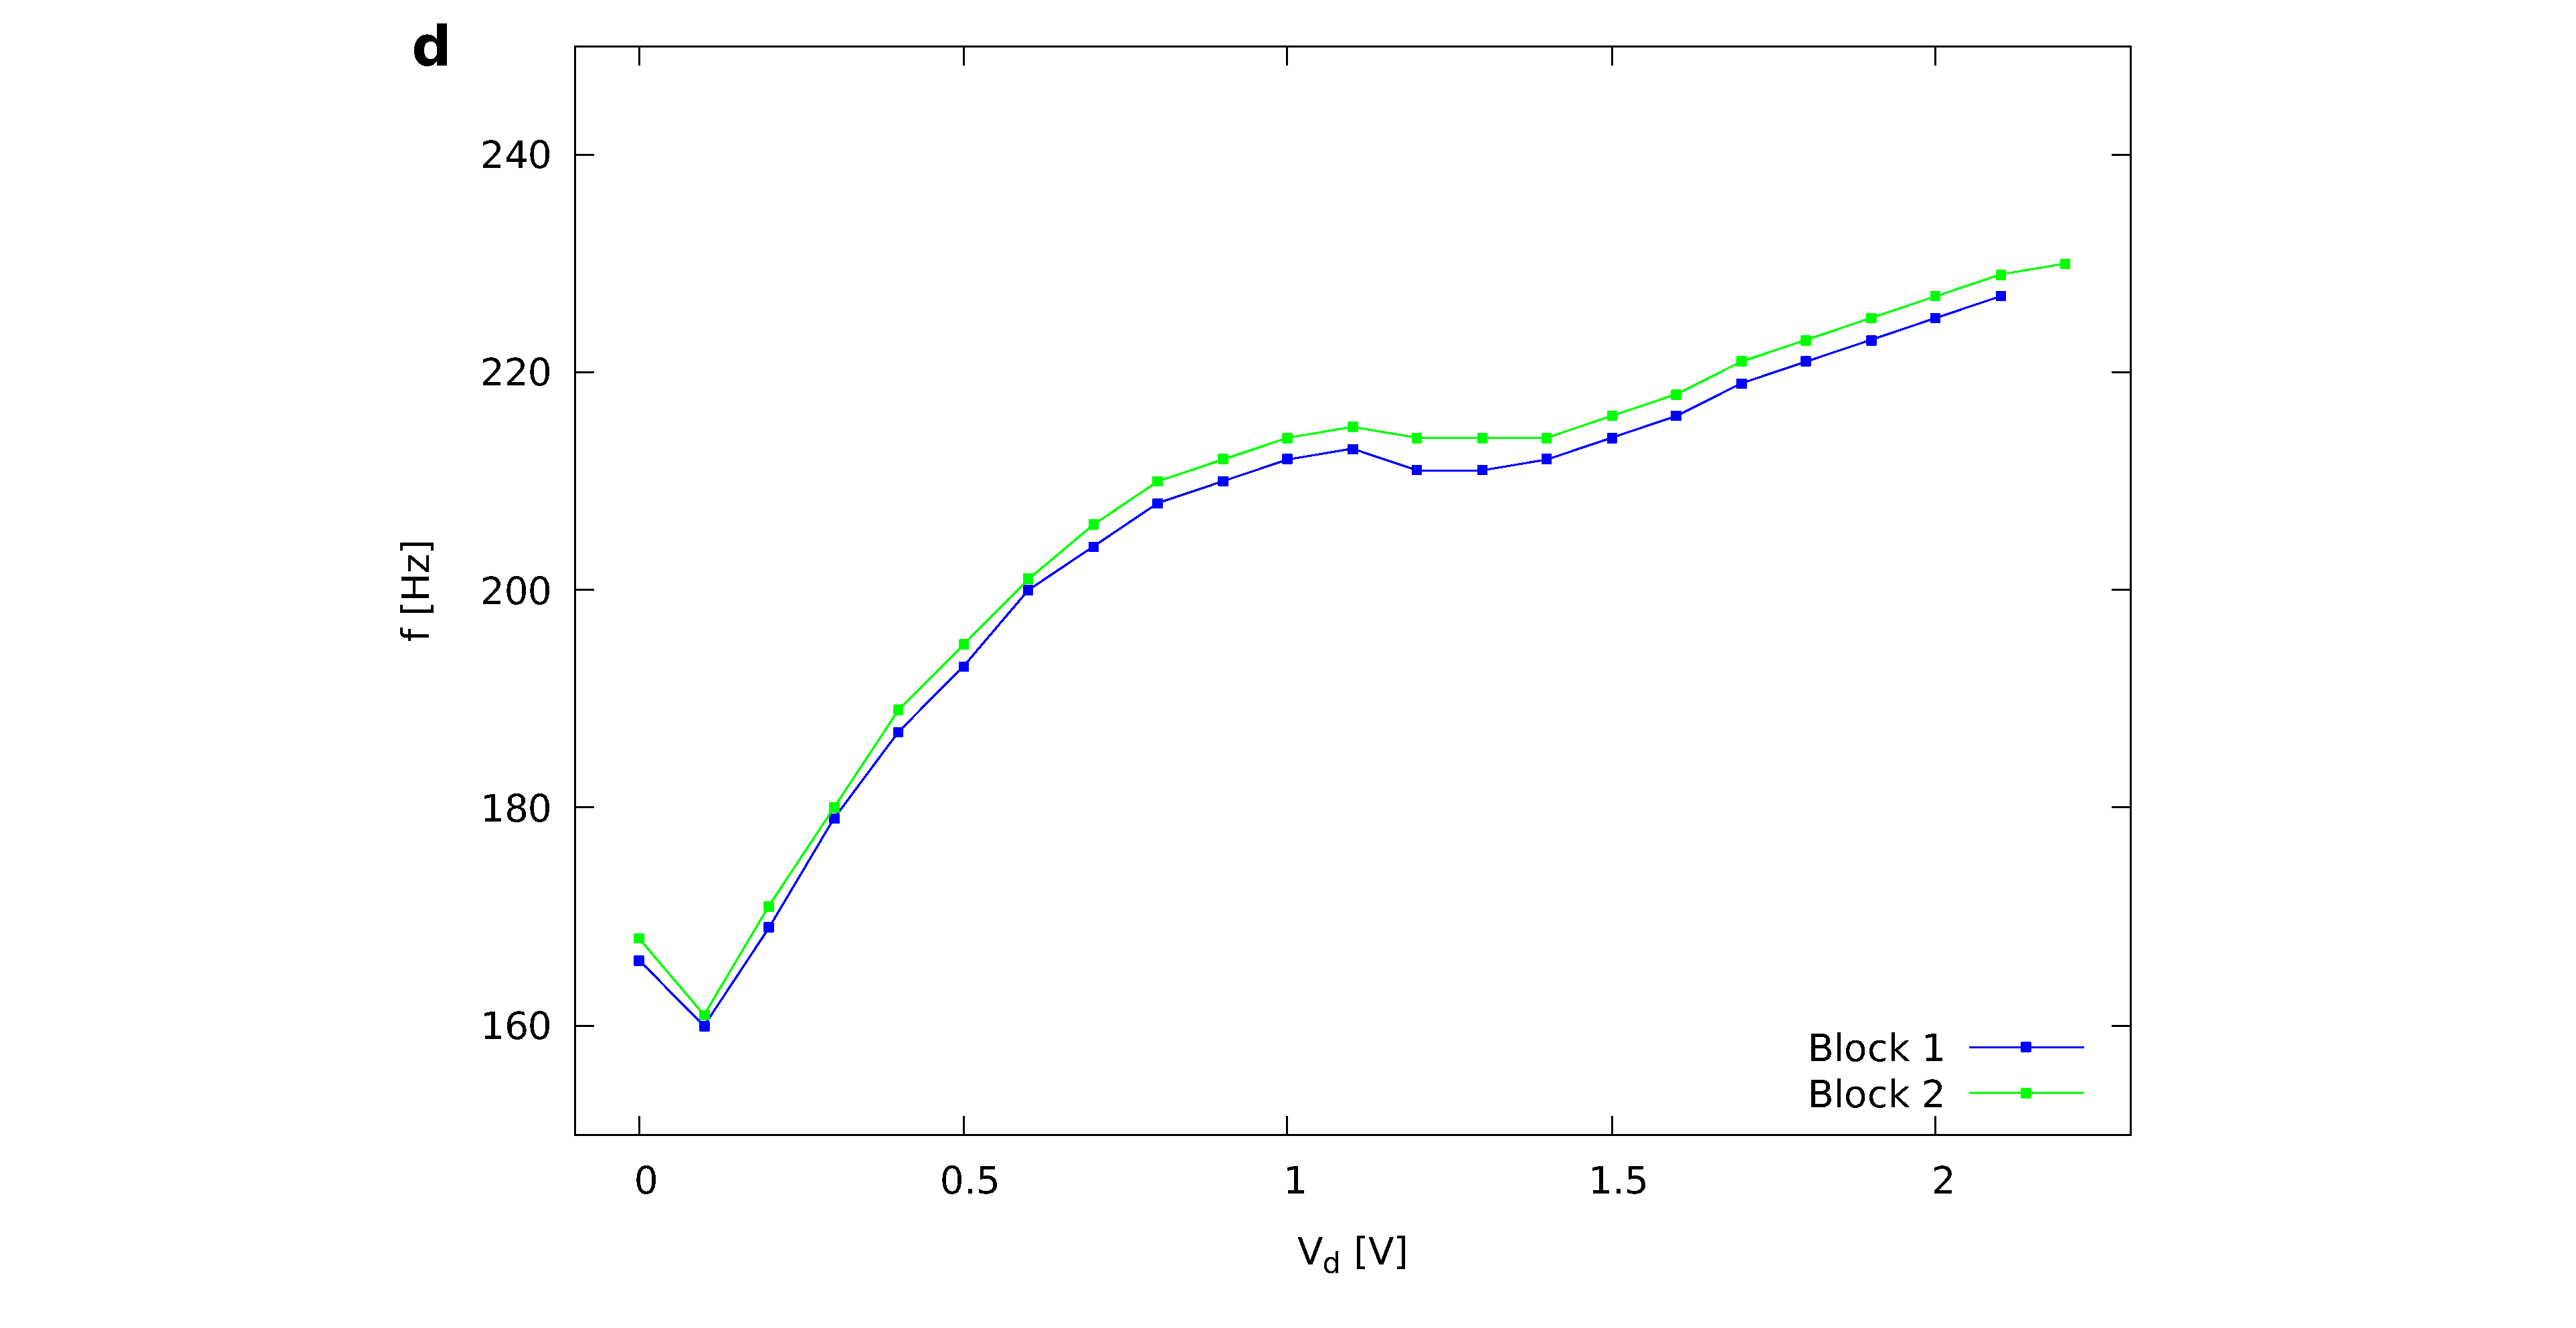
\includegraphics[width=\linewidth,trim={10cm 0 9cm 0},clip,left]
        {../1_block/board/freq_board.pdf}
    \end{subfigure}
    \begin{subfigure}{.49\textwidth}
        \centering
        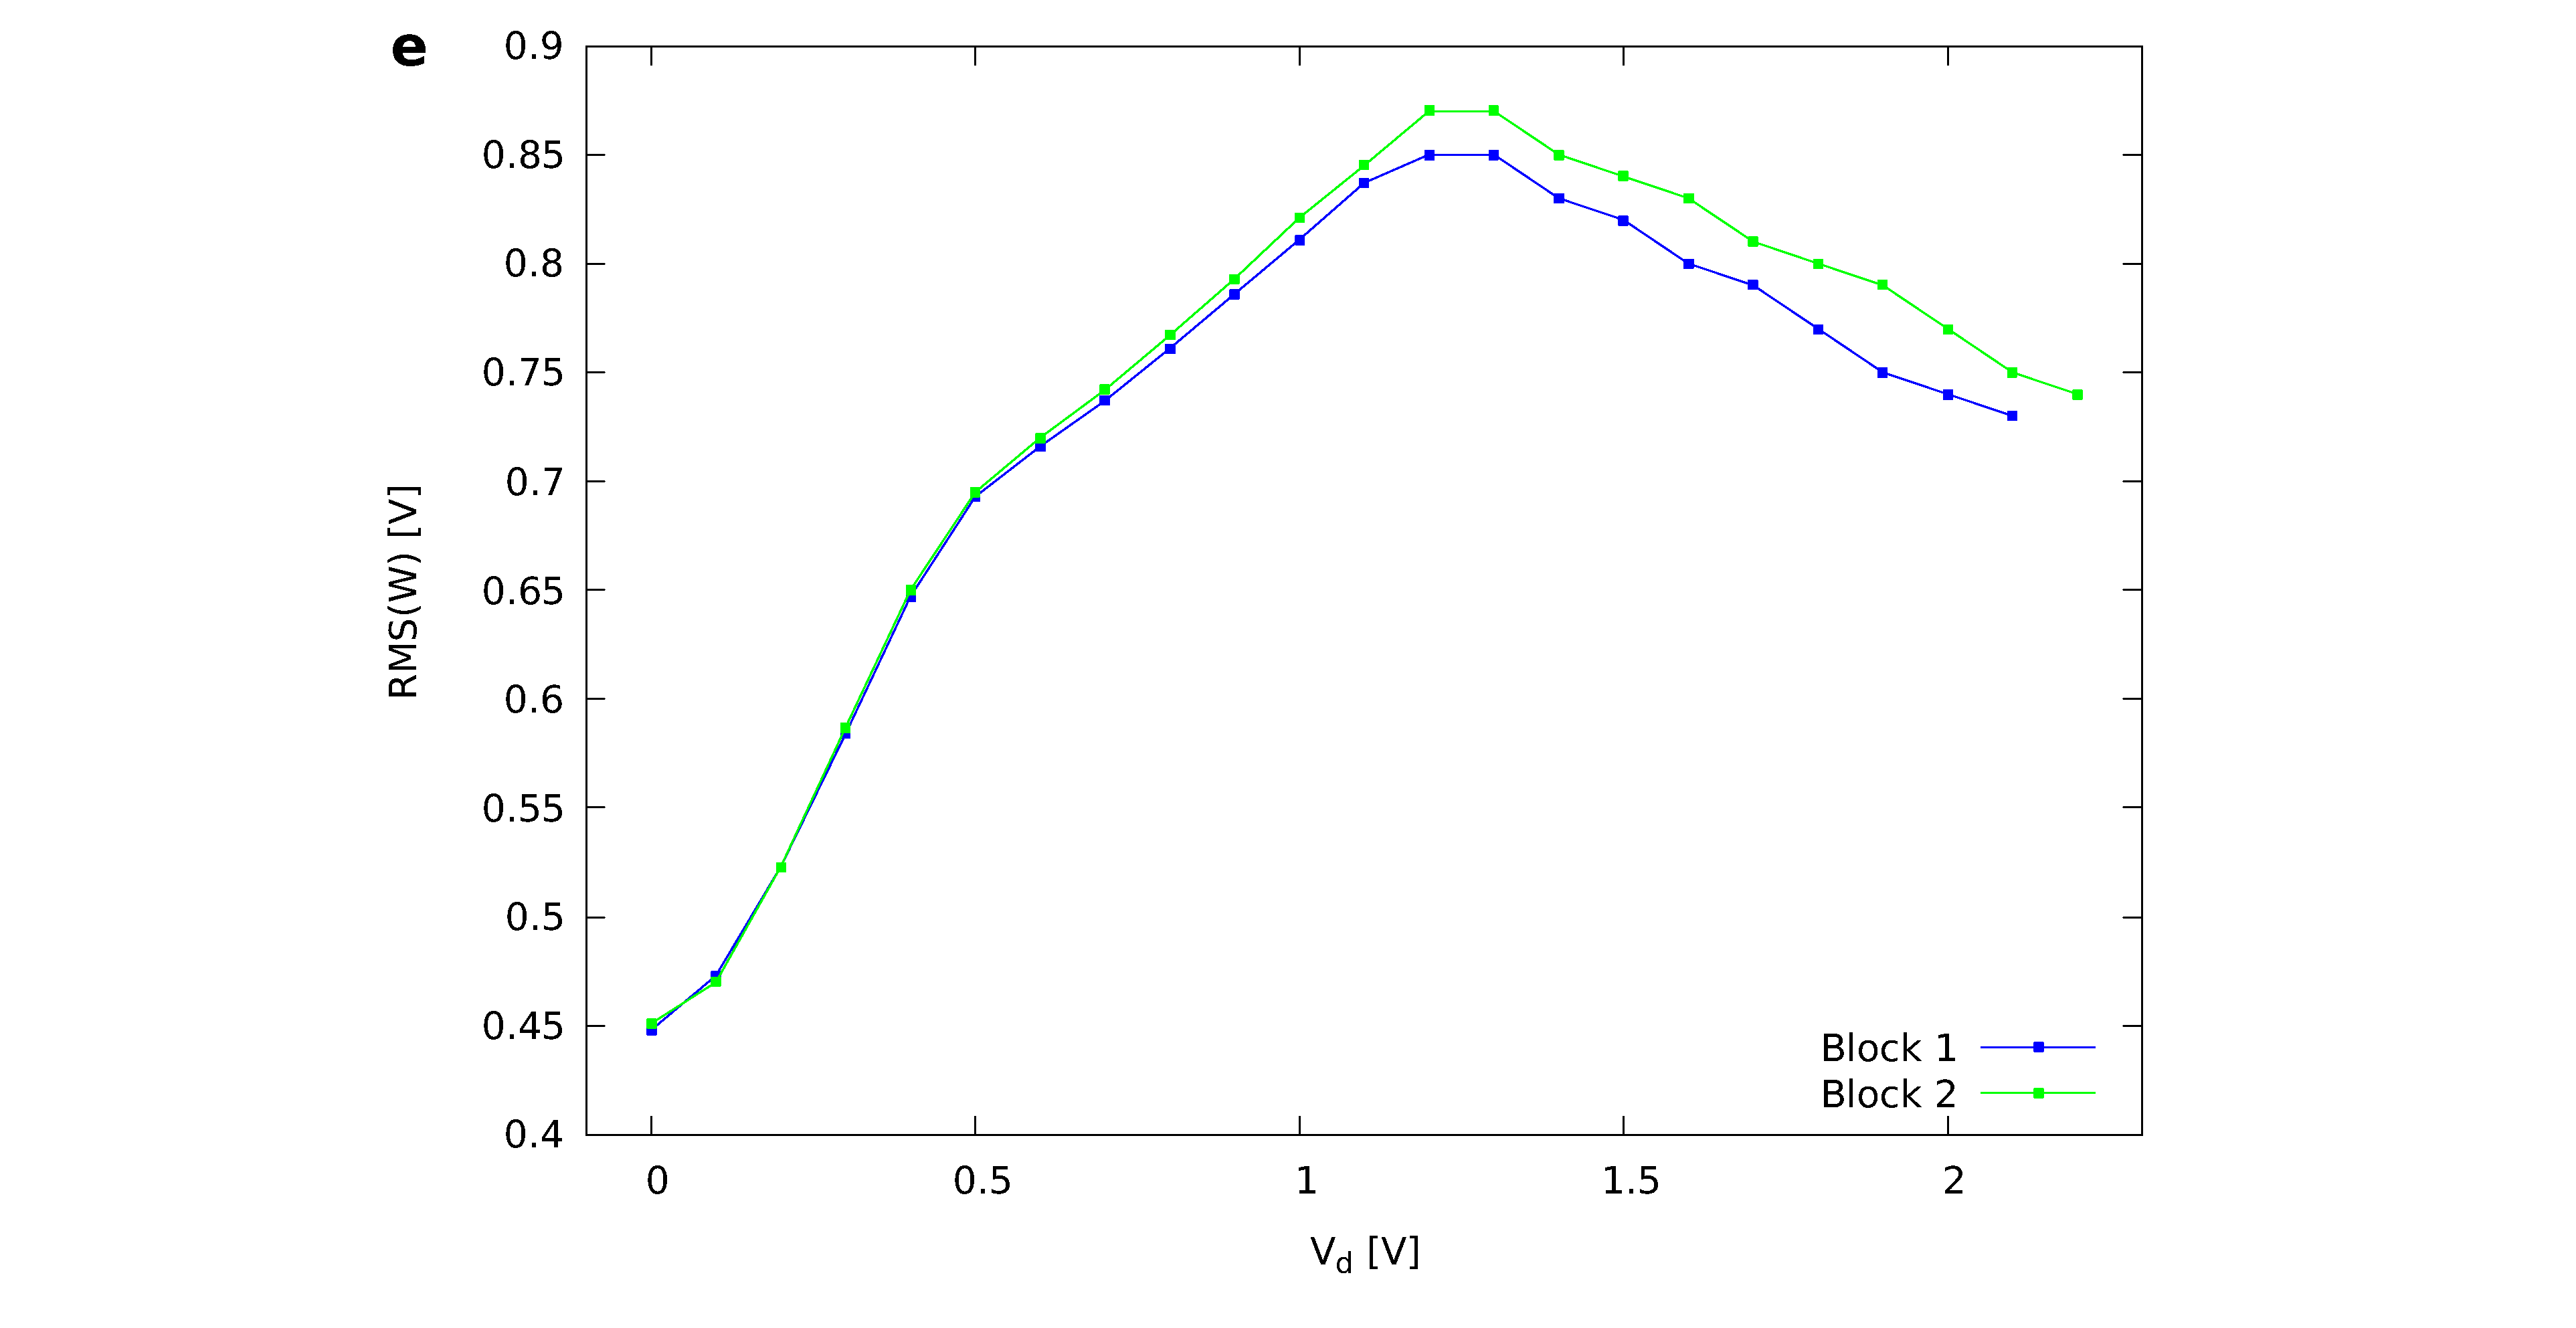
\includegraphics[width=\linewidth,trim={9cm 0 10cm 0},clip,right]
        {../1_block/board/rms_board.pdf}
    \end{subfigure}
    \caption{Oscillating behavior for the circuit implemented on
    the board. (a) Plot of $W$ and (b) of $V$ as a
    function of time, for $V_d=1$ V.
    (c) Phase portrait (Lissajous figure) of $V$ versus $W$. (d)
    Frequency and (e) root mean square amplitude of the
    output signal $W$ as a function of the parameter $V_d$ and for
    two different blocks.}
    \label{fig:oscillation board}
\end{figure}


\subsection{New board}\label{sec:new board}

\begin{figure}[H]
    \centering
    \begin{minipage}{.58\textwidth}
        \begin{subfigure}{\linewidth}
            \centering
            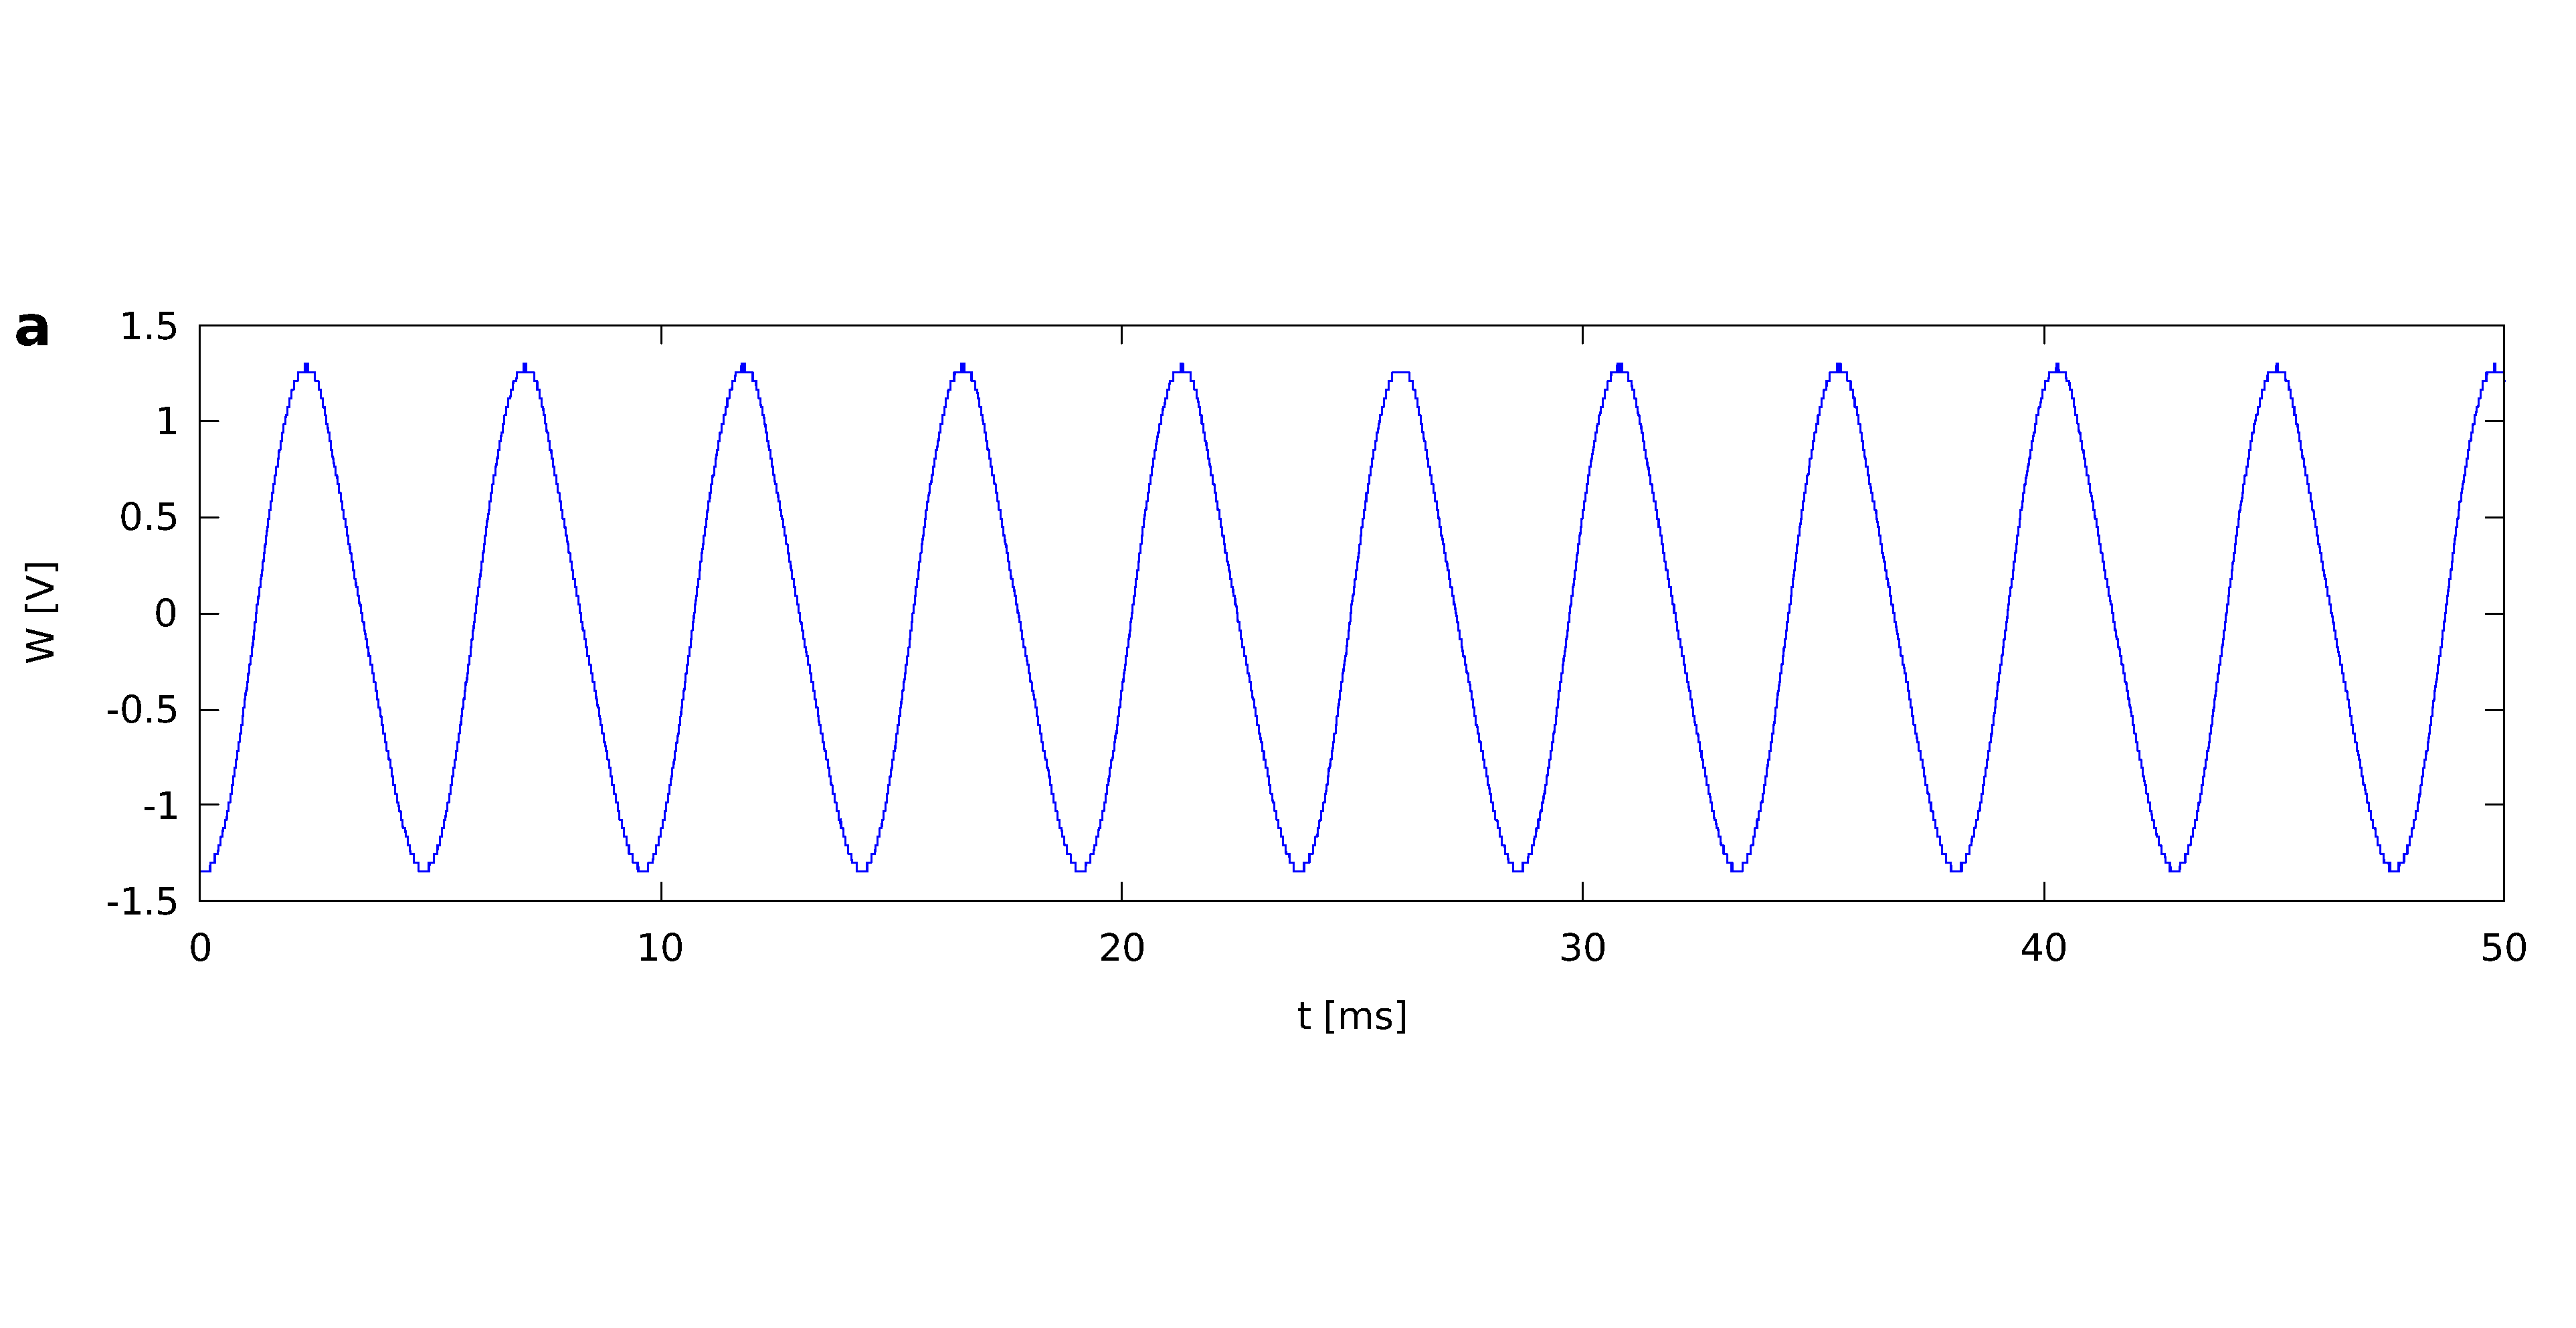
\includegraphics[width=\linewidth,trim={0 6cm 0 6cm},clip,left]
            {../1_block/board_new/W_wf.pdf}\\
            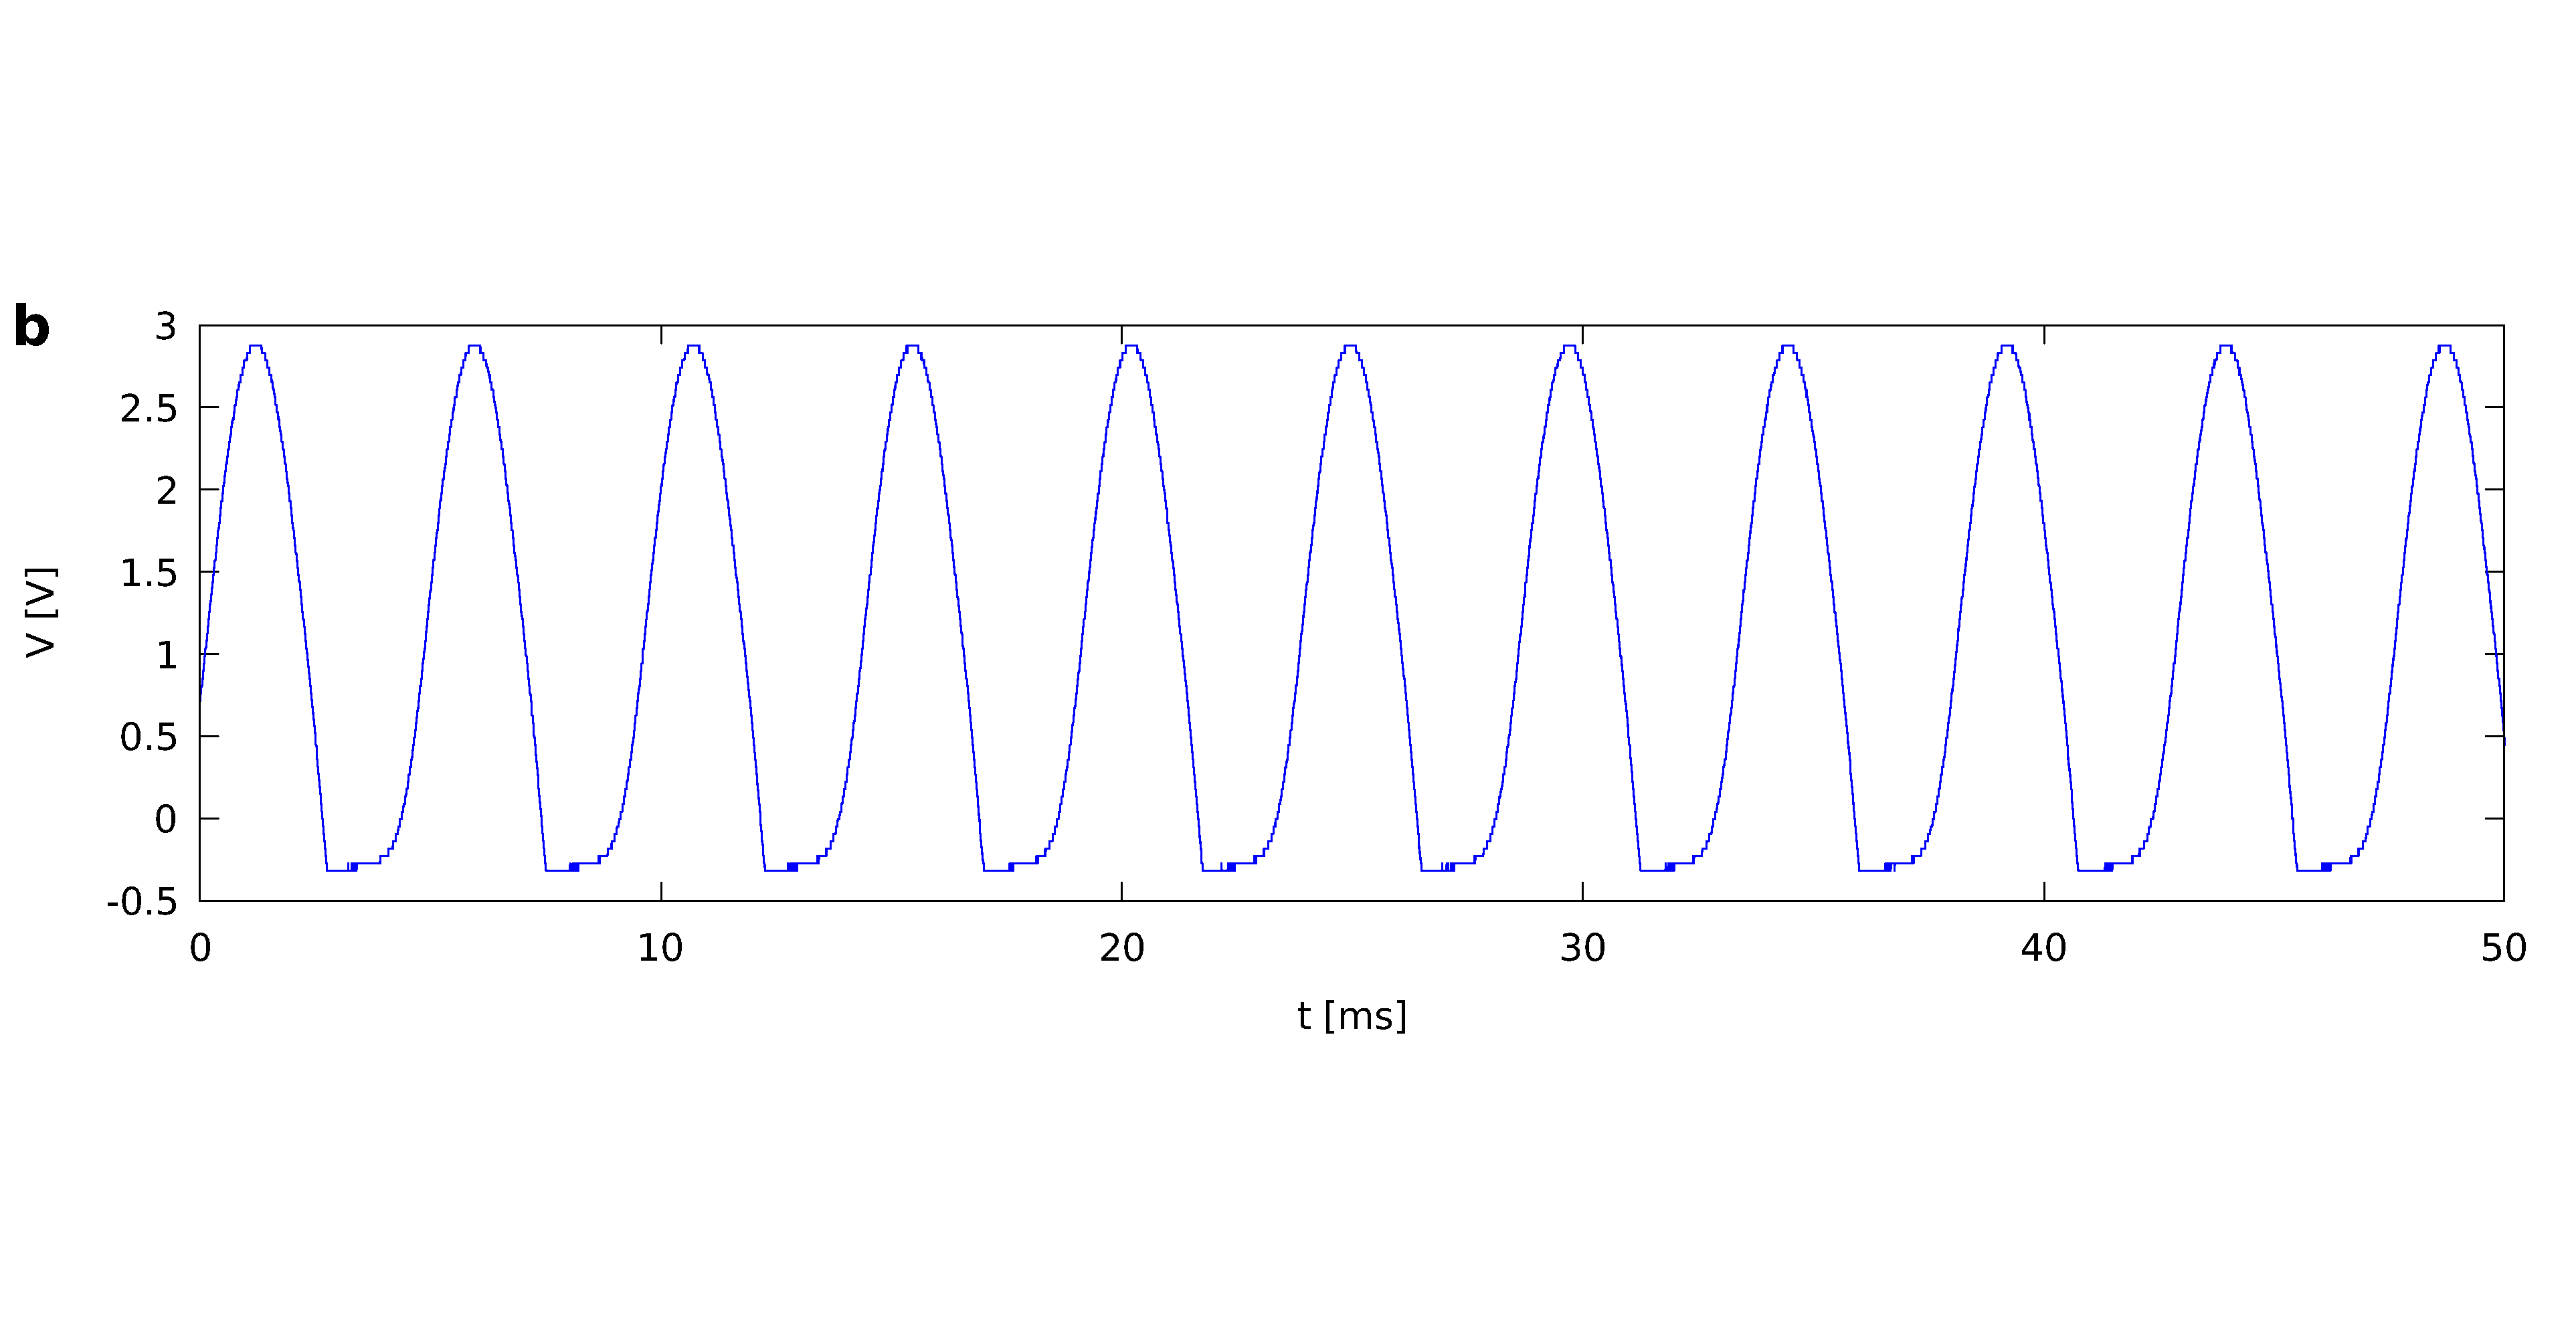
\includegraphics[width=\linewidth,trim={0 6cm 0 6cm},clip,left]
            {../1_block/board_new/V_wf.pdf}
        \end{subfigure}
    \end{minipage}
    \begin{subfigure}{.39\textwidth}
        \centering
        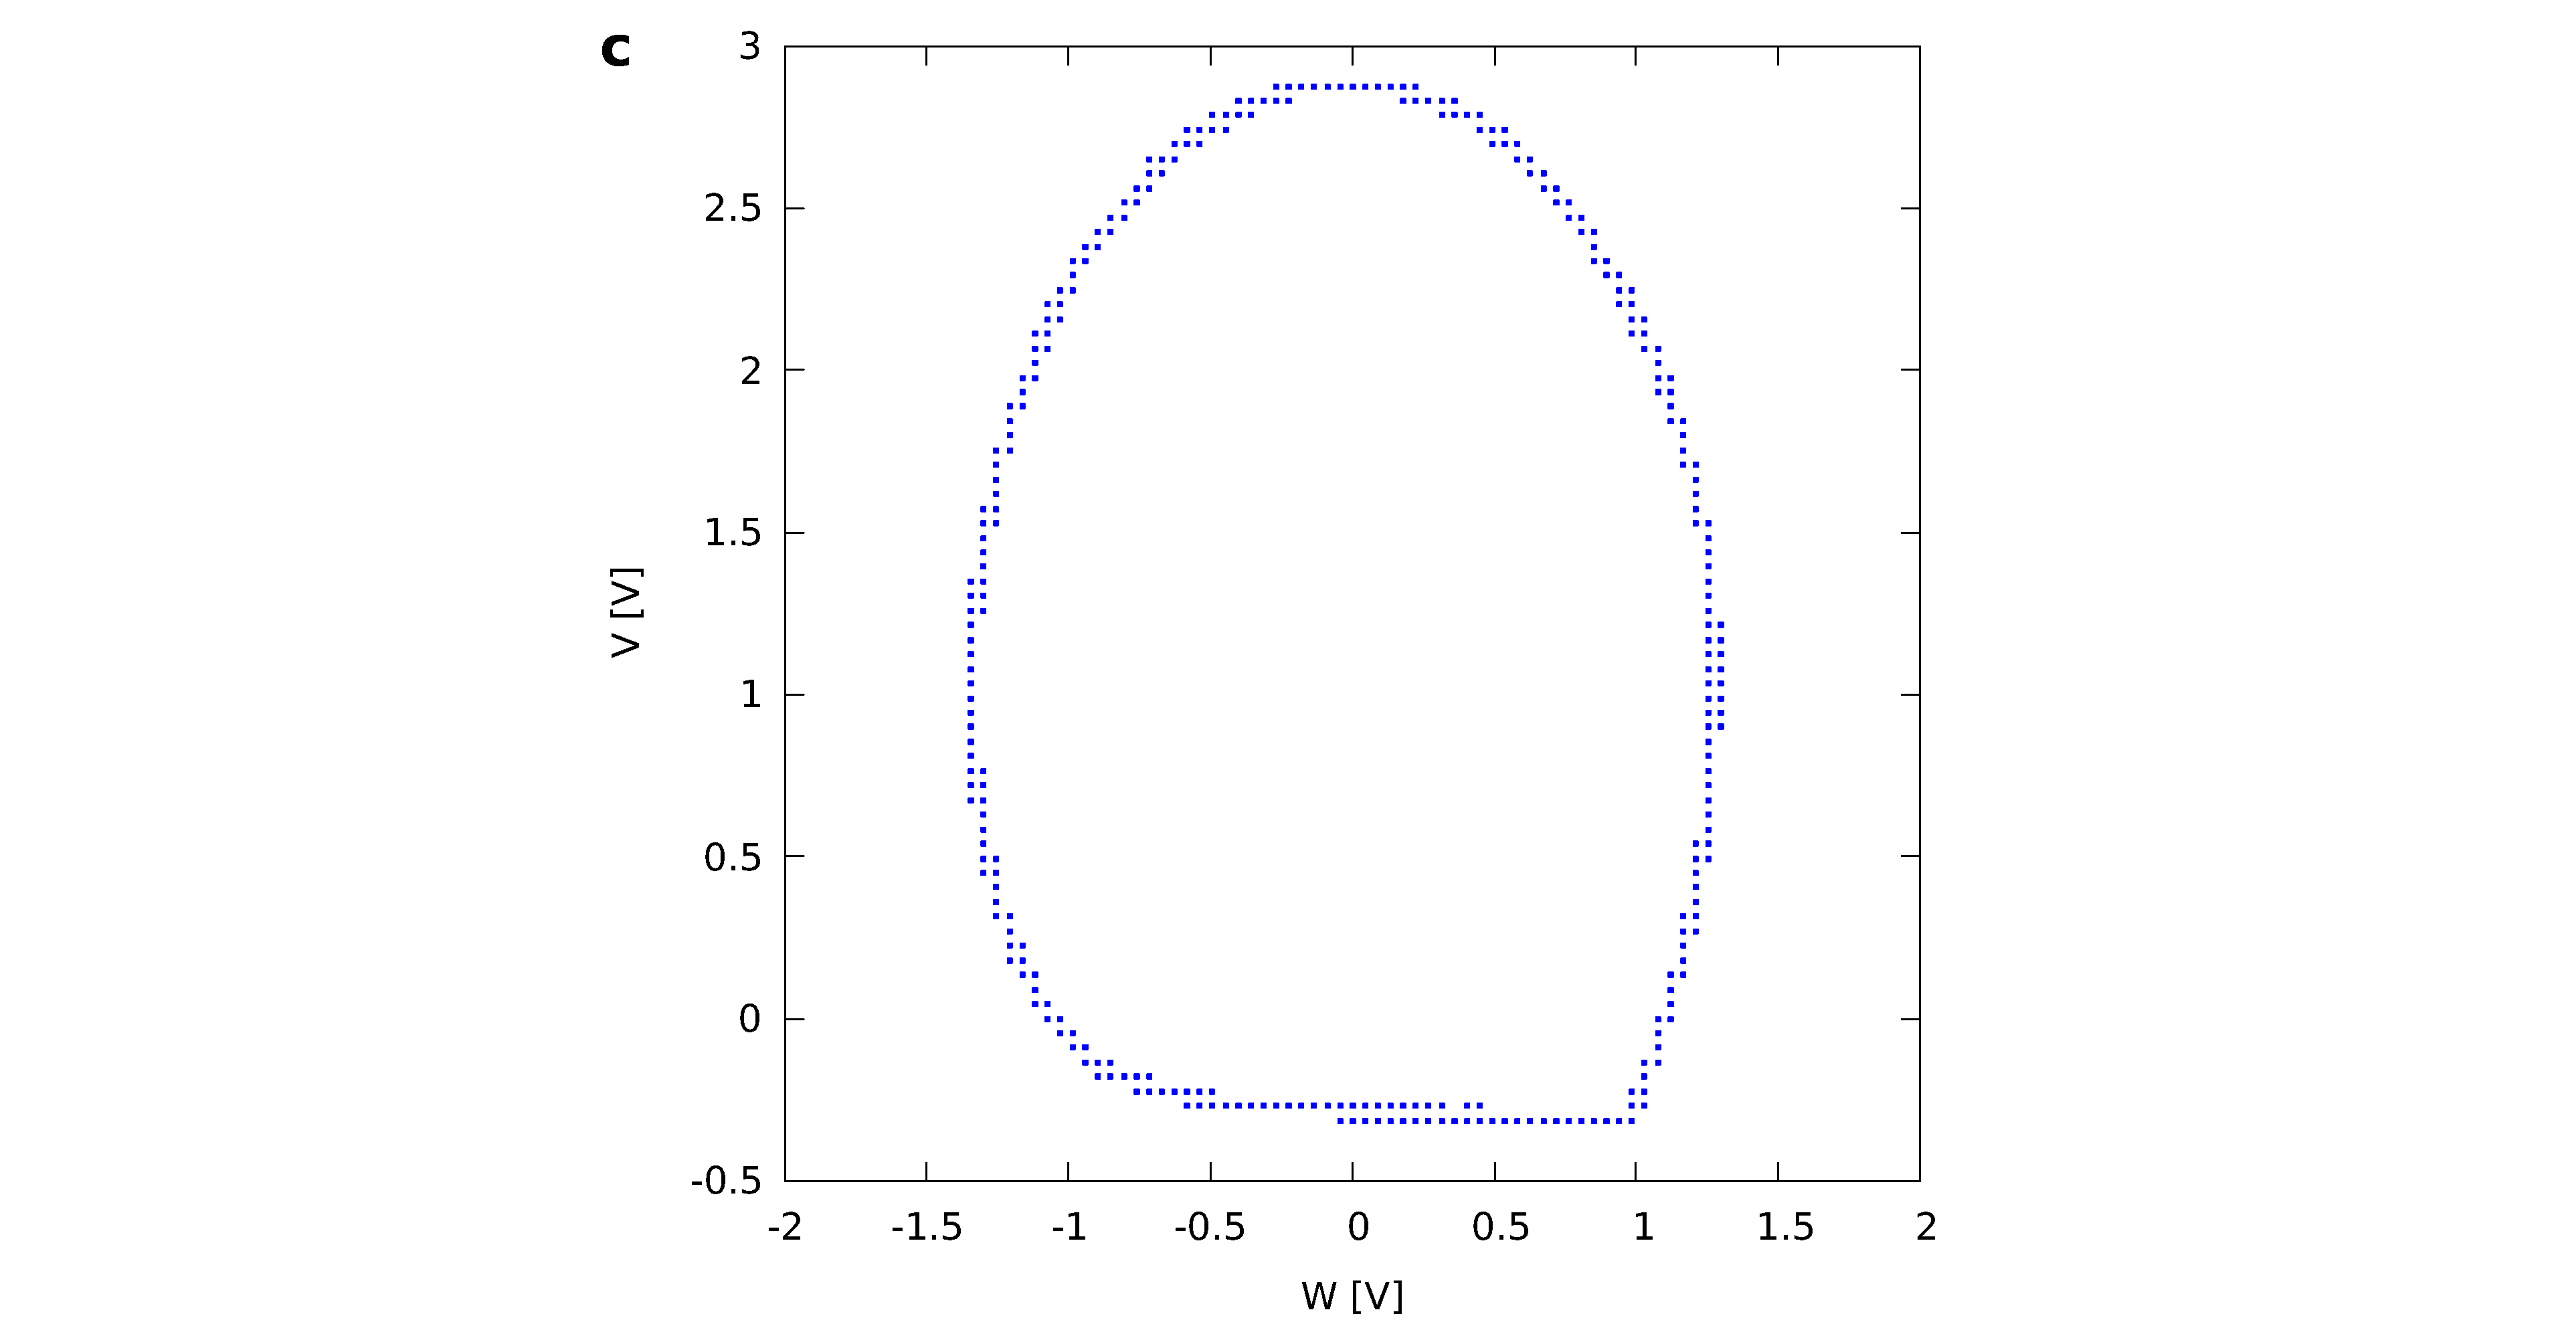
\includegraphics[width=\linewidth,trim={15cm 0 15cm 0},clip,right]
        {../1_block/board_new/Lissajous.pdf}
    \end{subfigure}
    \begin{subfigure}{.49\textwidth}
        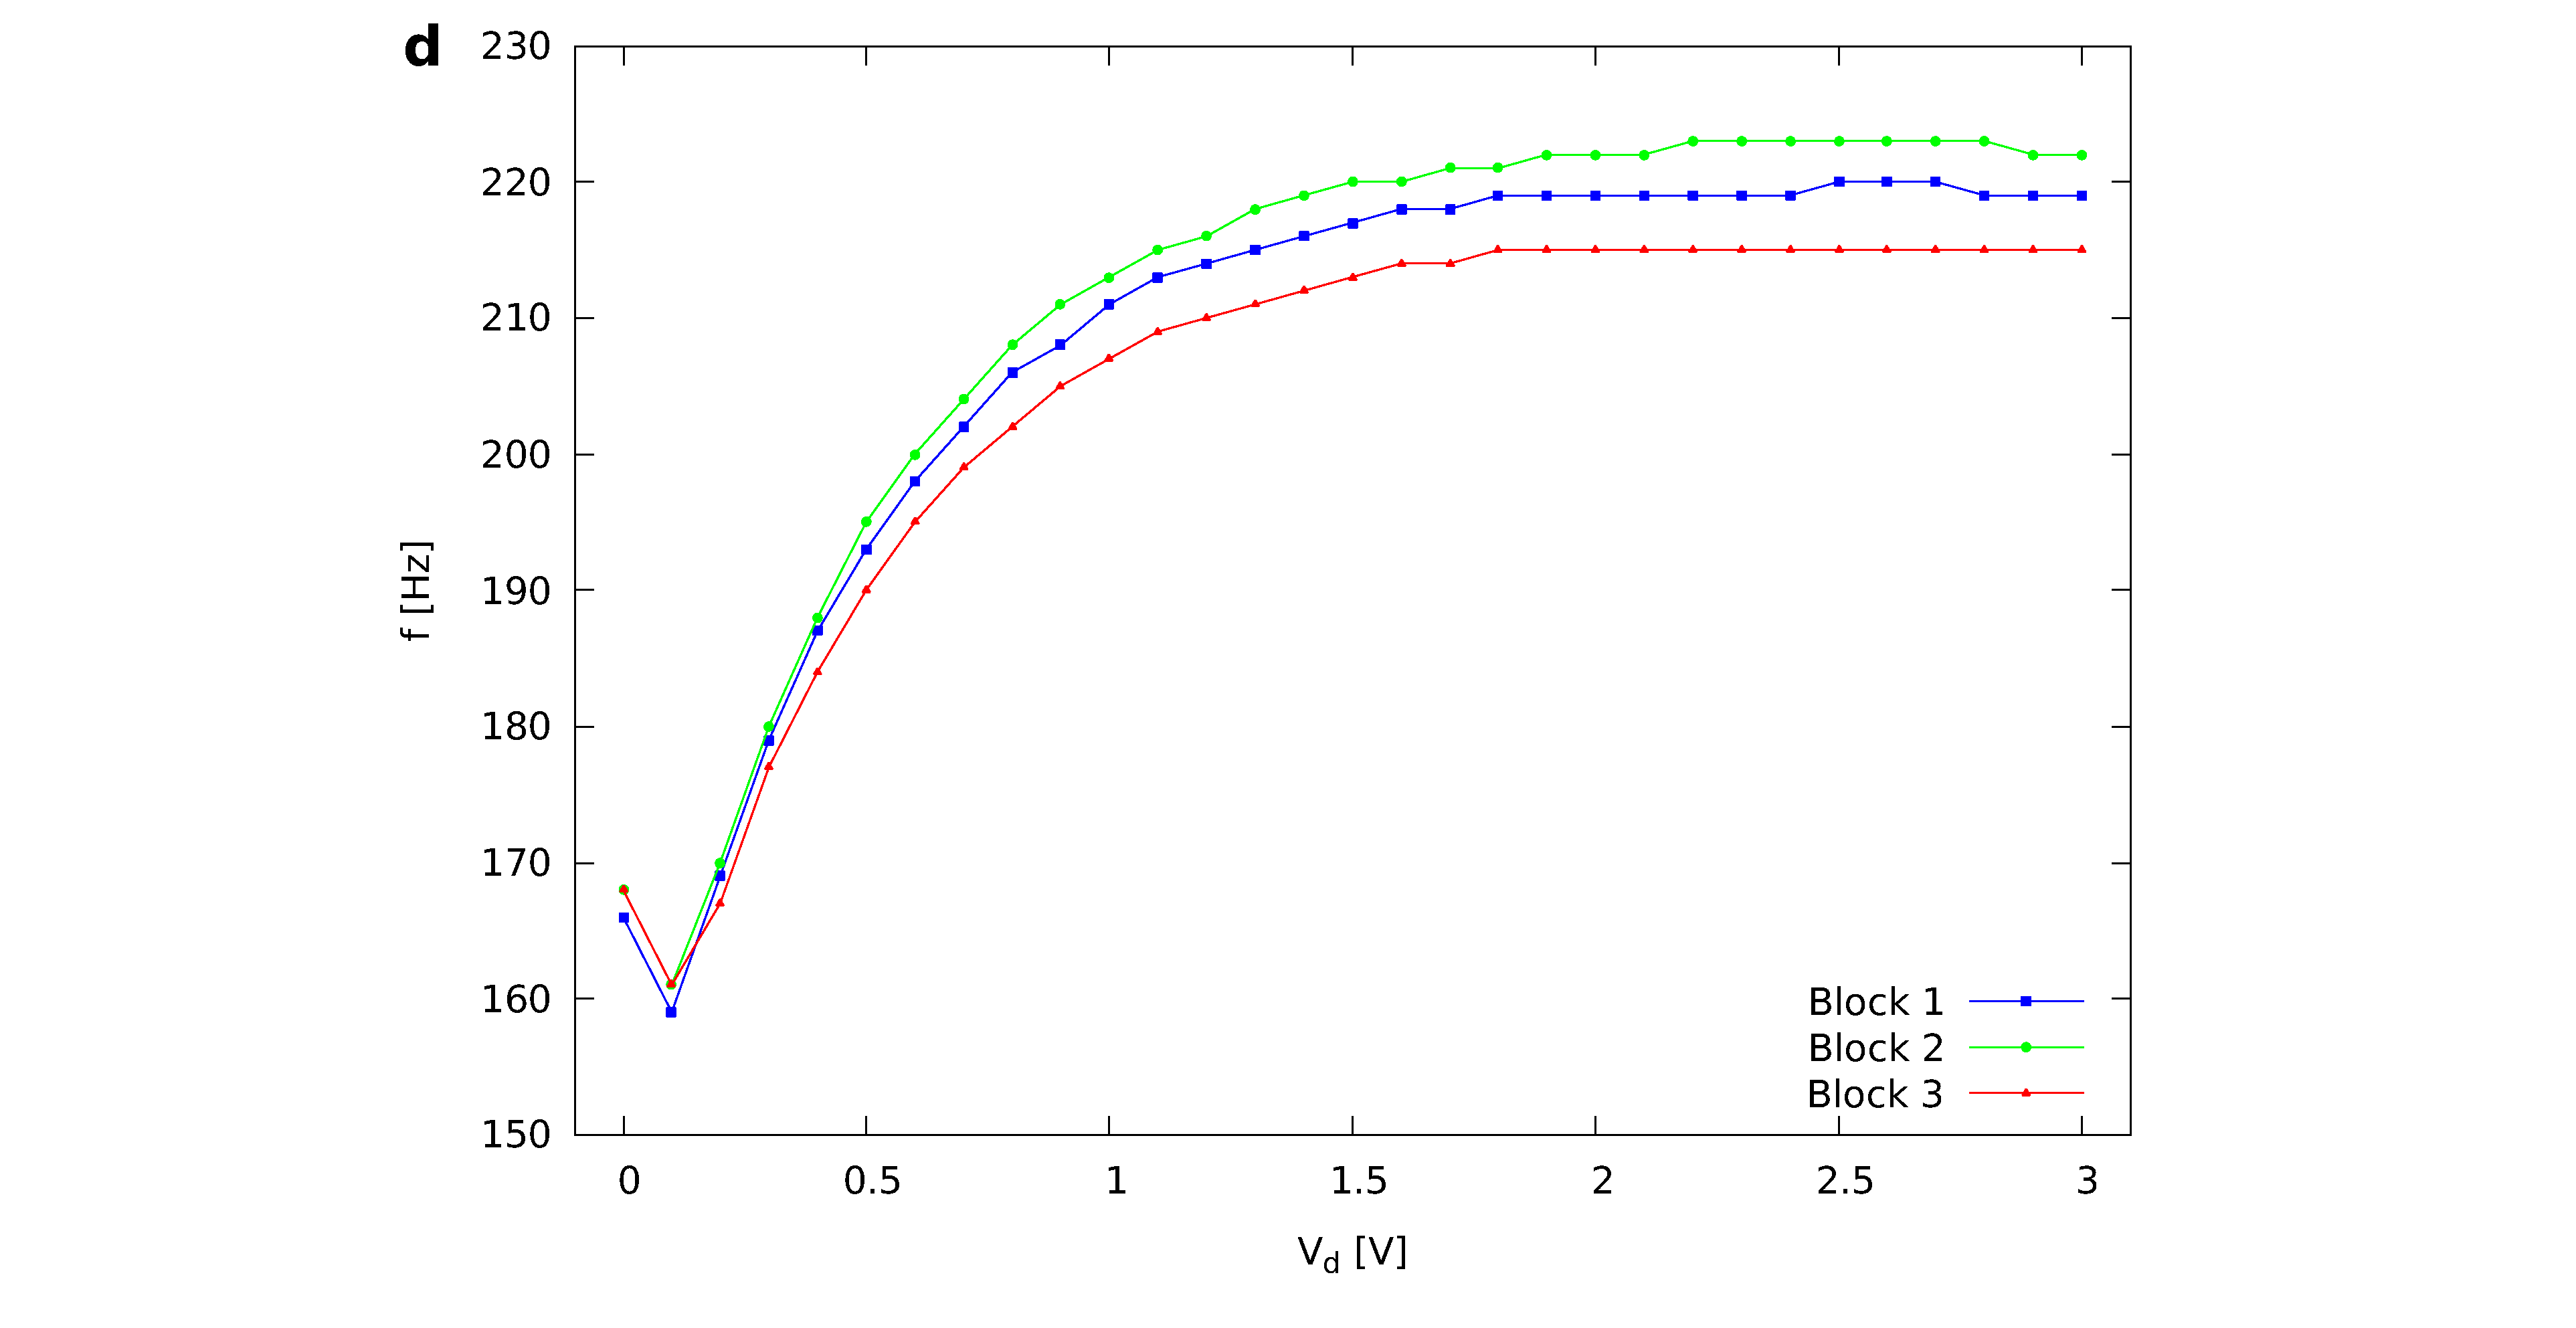
\includegraphics[width=\linewidth,trim={10cm 0 9cm 0},clip,left]
        {../1_block/board_new/freq_board.pdf}
    \end{subfigure}
    \begin{subfigure}{.49\textwidth}
        \centering
        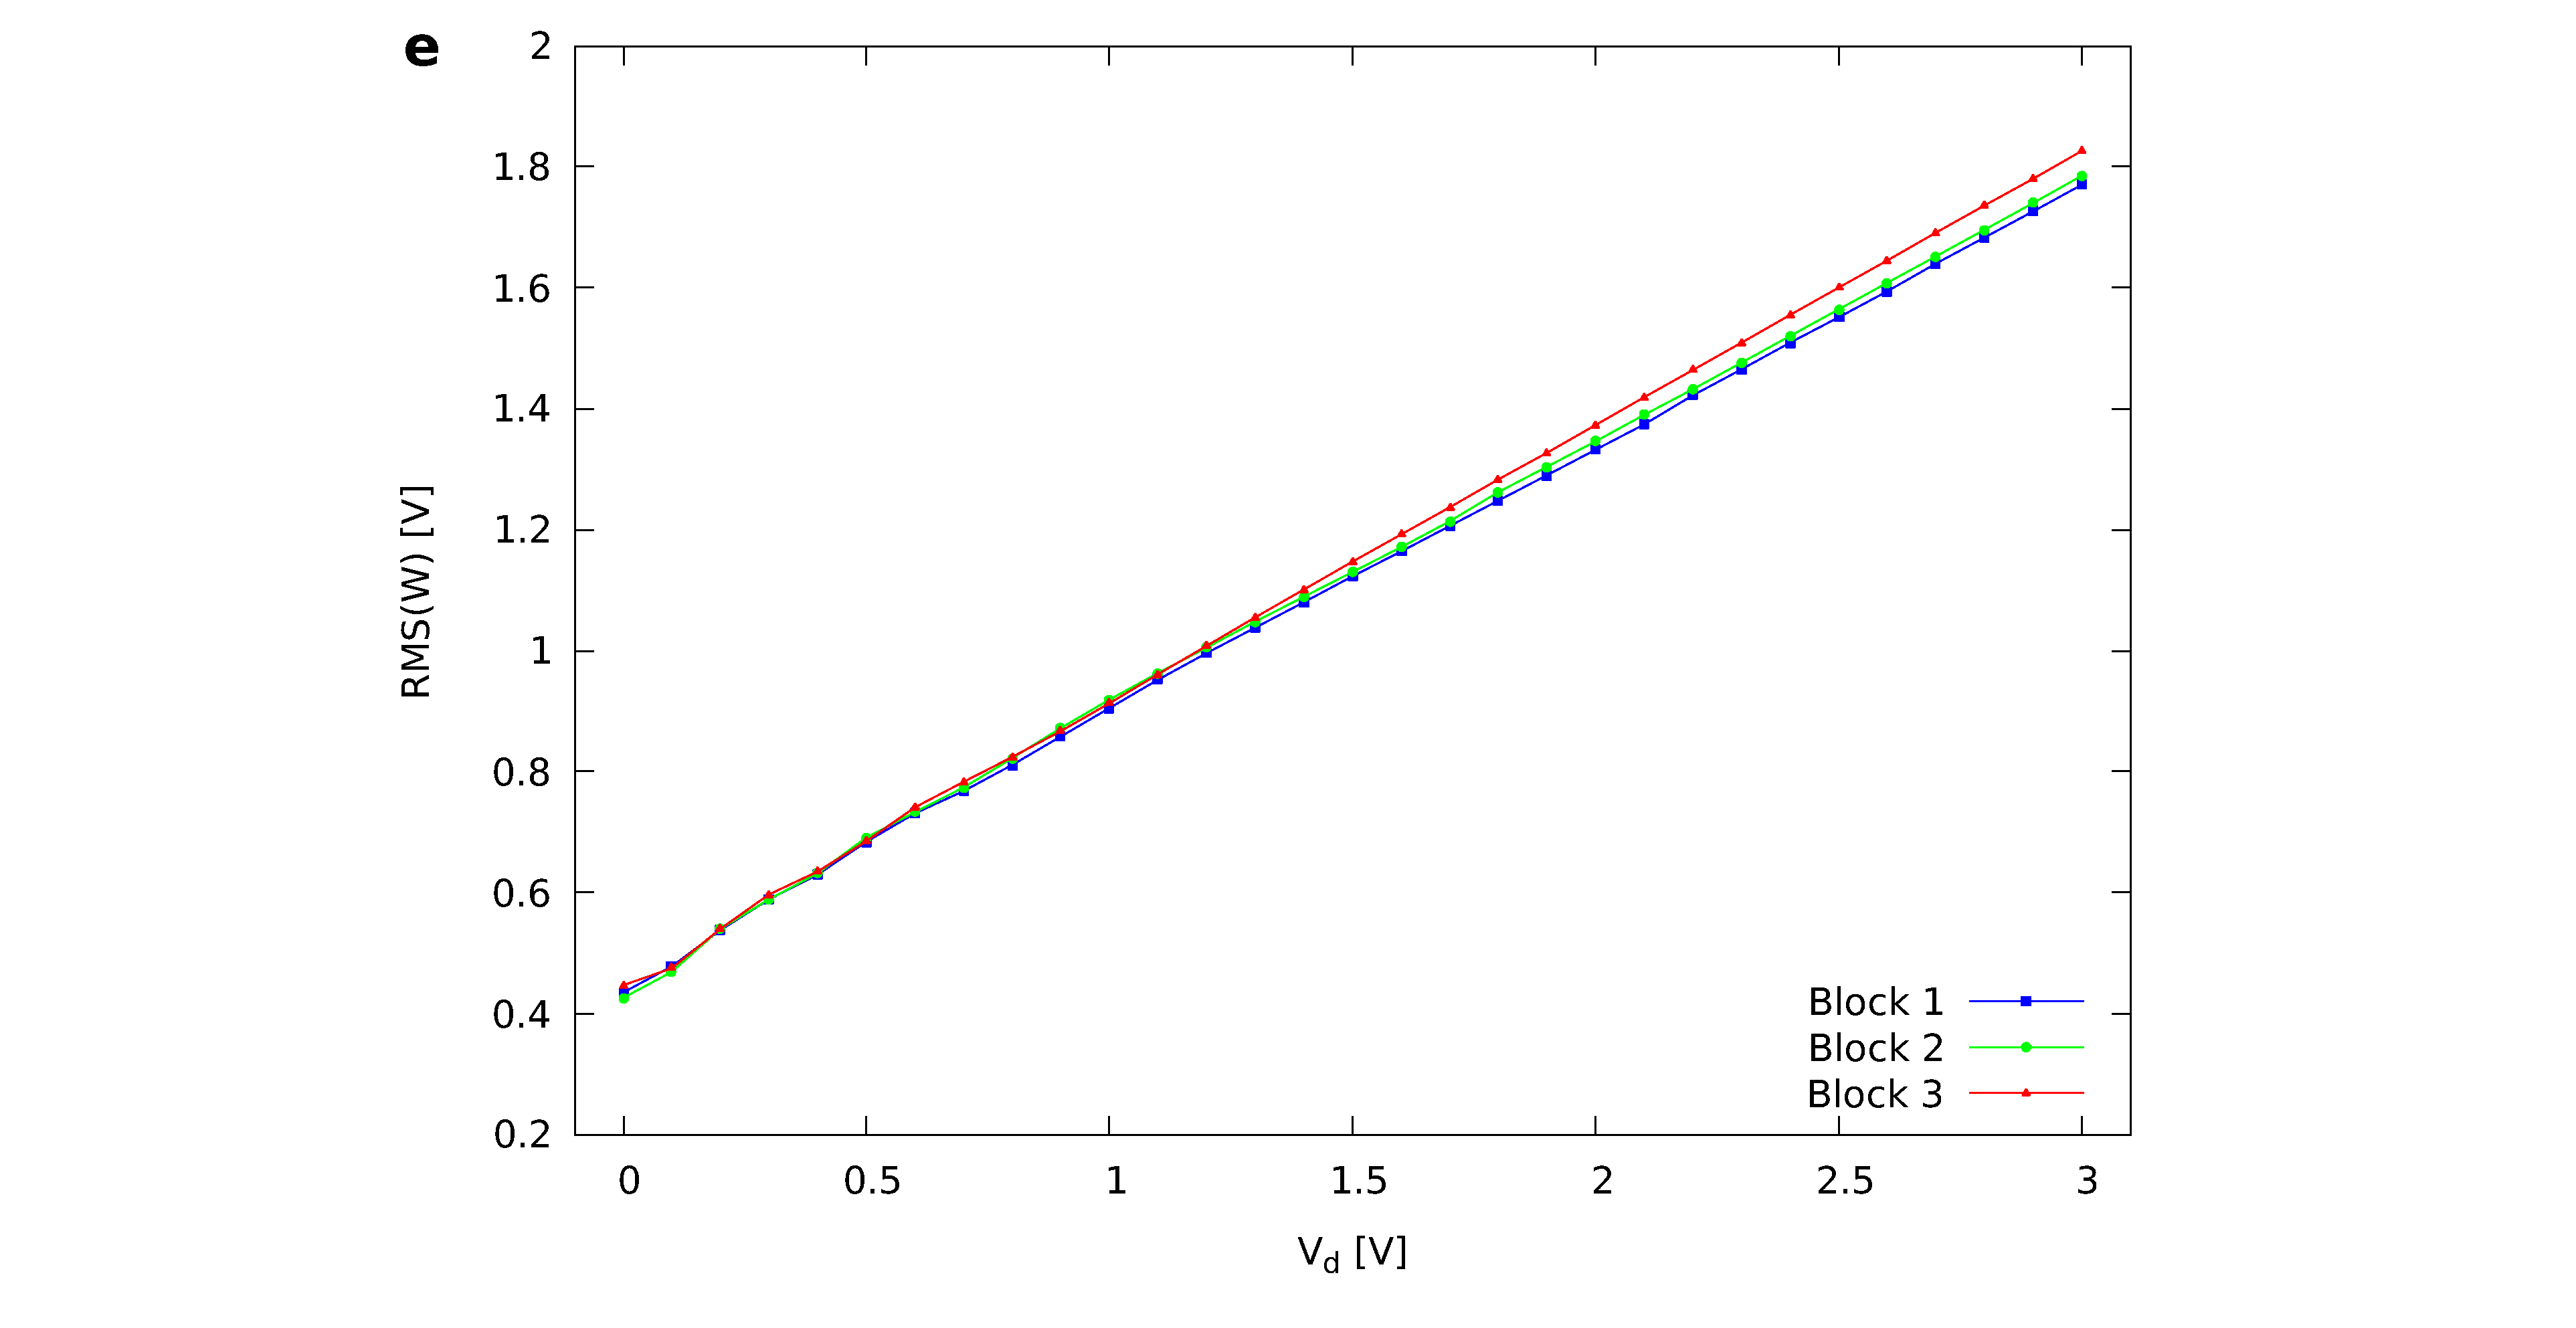
\includegraphics[width=\linewidth,trim={9cm 0 10cm 0},clip,right]
        {../1_block/board_new/rms_board.pdf}
    \end{subfigure}
    \caption{Oscillating behavior for the circuit implemented on
    the new board. (a) Plot of $W$ and (b) of $V$ as a
    function of time, for $V_d=1$ V.
    (c) Phase portrait (Lissajous figure) of $V$ versus $W$. (d)
    Frequency and (e) root mean square amplitude of the
    output signal $W$ as a function of the parameter $V_d$ and for
    three different blocks.}
    \label{fig:oscillation board new}
\end{figure}

\subsection{Conclusions}\label{sec:conclusions}

The comparison between frequency and amplitude on the three
implementations is shown in Fig. \ref{fig:comparison}.
The frequency of the board is very similar to the breadboard one
for voltages $V_d < 1$ V; at higher voltages there are small
deviations in the board, probably due to the increased relevance
of the current clamping. This might also be the reason why the
amplitude behavior of the board is not linear.

\begin{figure}[H]
    \centering
    \begin{subfigure}{.49\textwidth}
        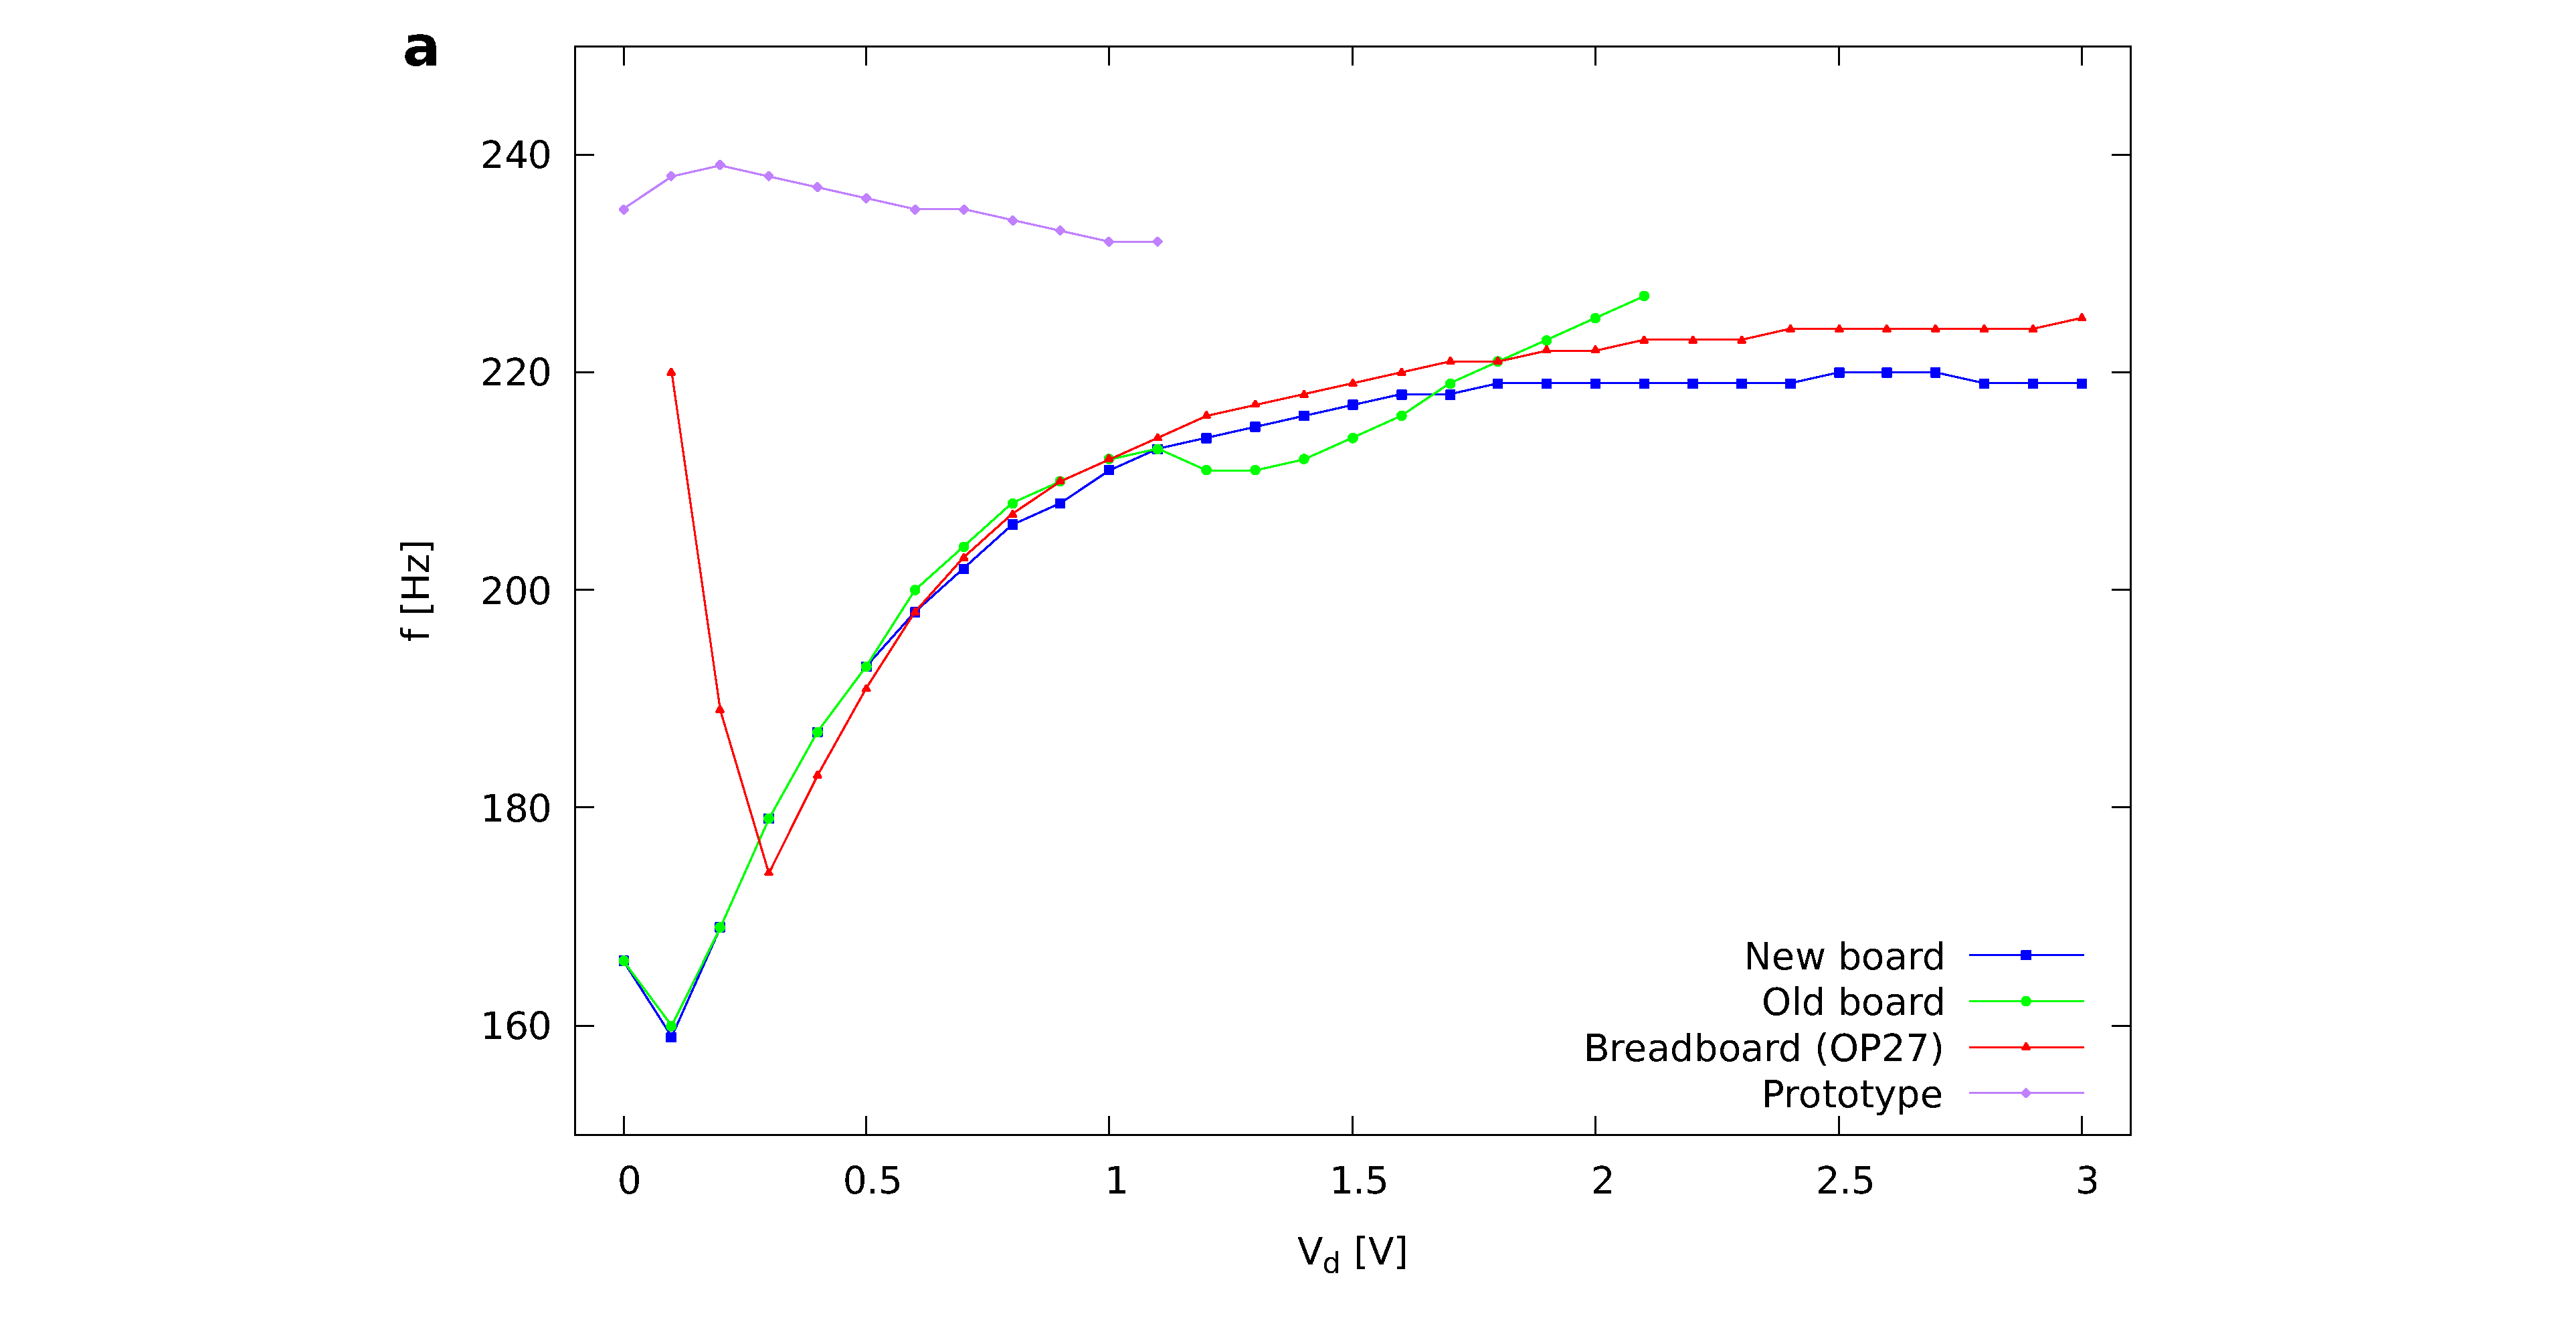
\includegraphics[width=\linewidth,trim={10cm 0 9cm 0},clip,left]
        {../1_block/images/freq_comparison.pdf}
    \end{subfigure}
    \begin{subfigure}{.49\textwidth}
        \centering
        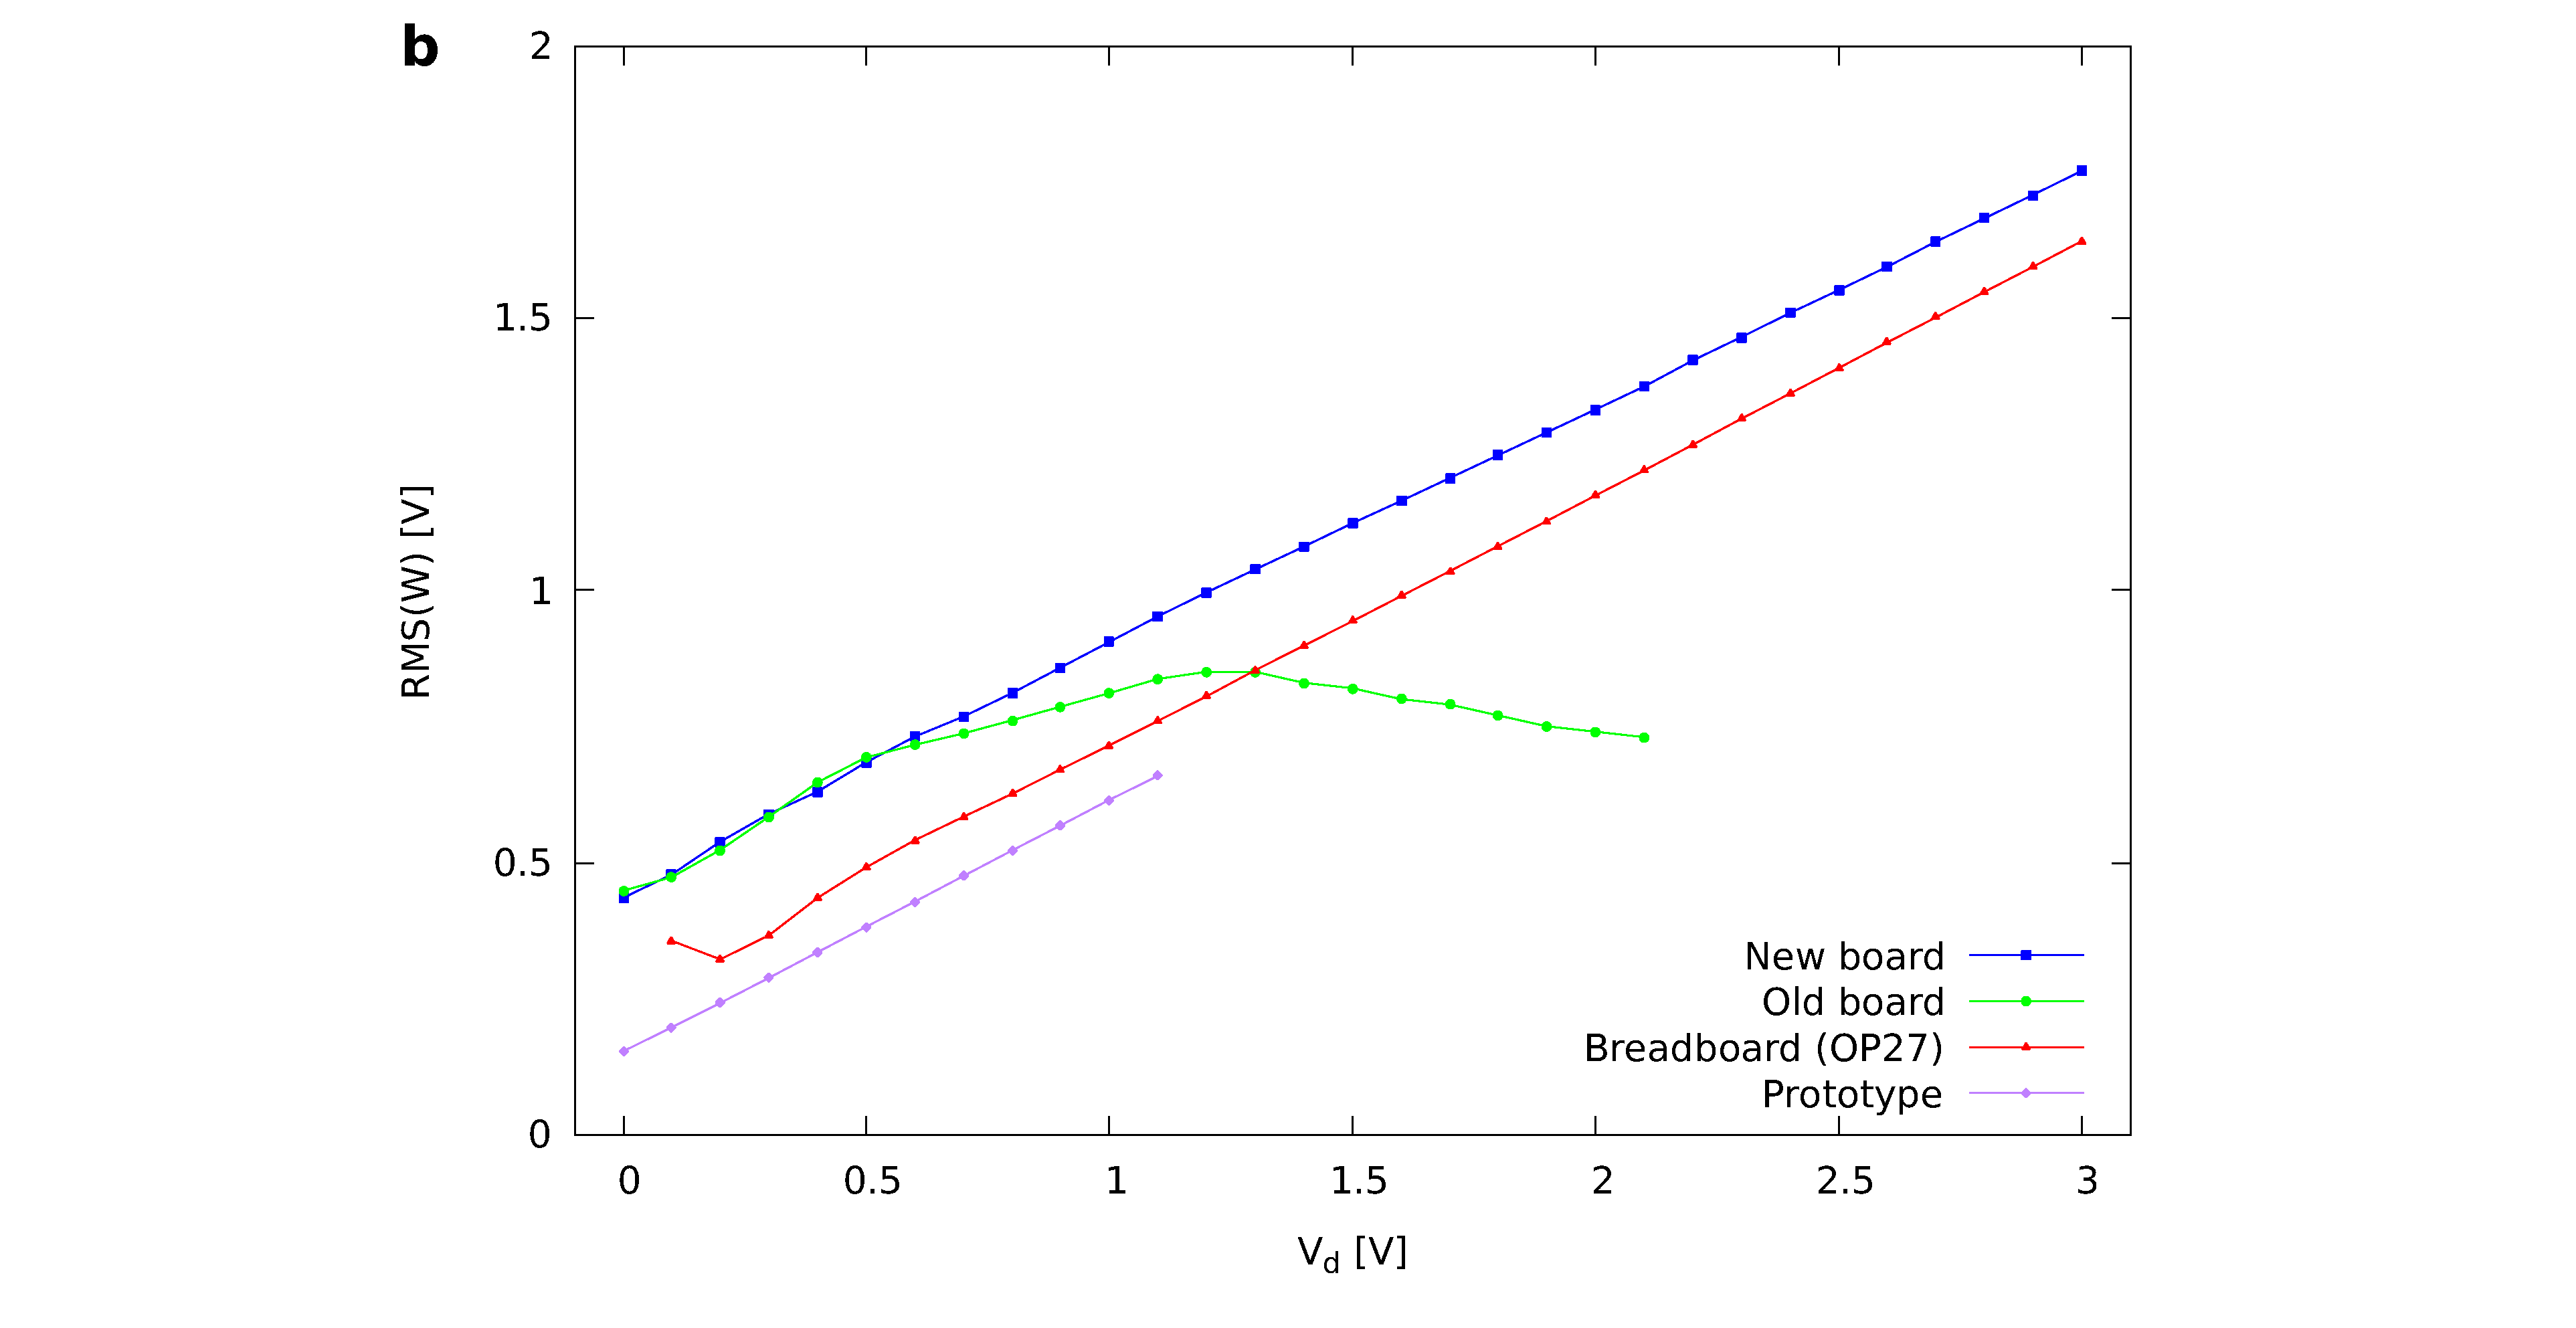
\includegraphics[width=\linewidth,trim={9cm 0 10cm 0},clip,right]
        {../1_block/images/rms_comparison.pdf}
    \end{subfigure}
    \caption{(a) Frequency and (b) root mean square amplitude
    of the output signal $W$ as a function of the parameter $V_d$
    for the three implementations of the BK model, i.e. the first
    block of the board, the breadboard implementation with the
    OP27 op-amps and the first prototypical chip.}
    \label{fig:comparison}
\end{figure}

\clearpage

\section{Multi block measurements}

\subsection{Two blocks}

The coupling between two oscillators is performed by connecting
the inverted voltage $-W_2$ of the second oscillator to the
first one and viceversa, as shown in Fig.
\ref{fig:breadboard implementation}. A chaotic behavior can be observed,
as can be seen in Fig. \ref{fig:2 blocks waveforms}.


\begin{figure}[H]
    \centering
    \begin{minipage}{.49\textwidth}
        \begin{subfigure}{\linewidth}
            \centering
            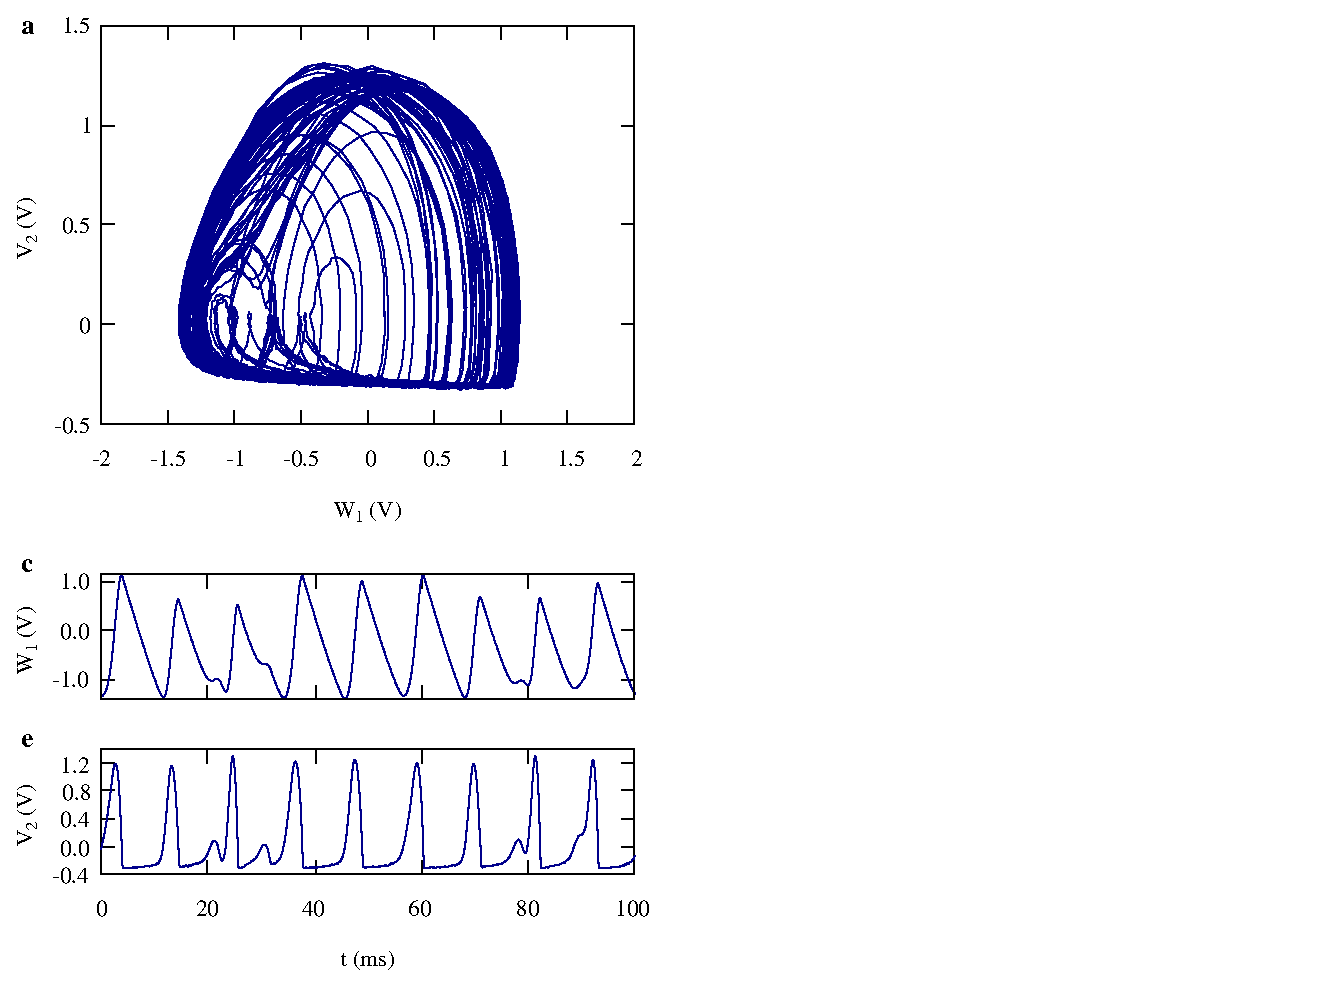
\includegraphics[width=\linewidth,trim={0cm 0 11cm 0},clip,center]
            {../2_blocks/4e4_points/plots/waveforms_1.pdf}
        \end{subfigure}
    \end{minipage}
    \begin{minipage}{.49\textwidth}
        \begin{subfigure}{\linewidth}
            \centering
            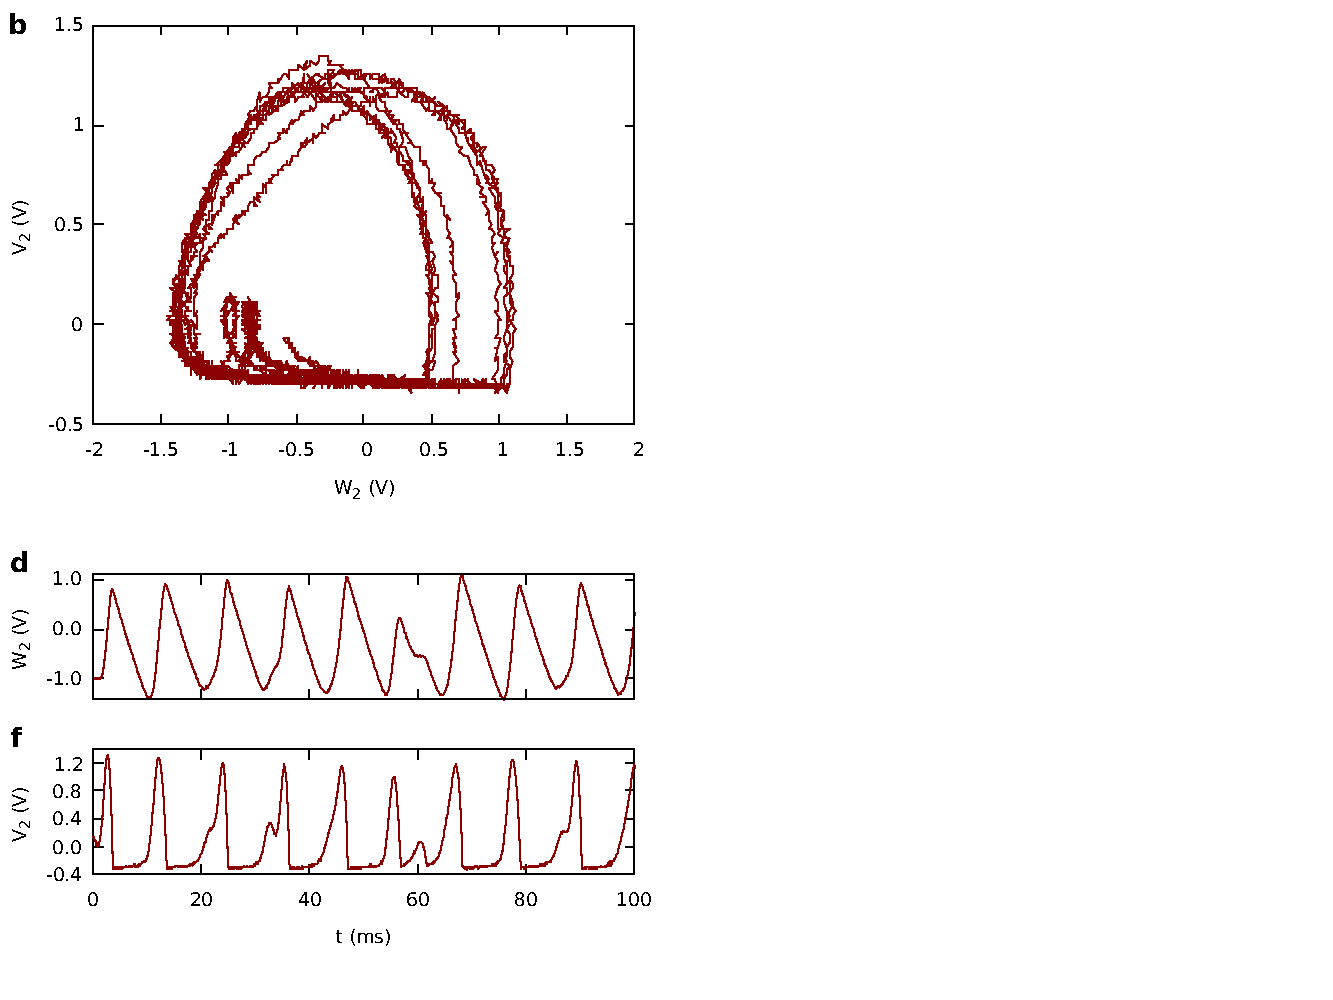
\includegraphics[width=\linewidth,trim={0cm 0 11cm 0},clip,center]
            {../2_blocks/4e4_points/plots/waveforms_2.pdf}
        \end{subfigure}
    \end{minipage}
    \caption{Chaotic behavior of two coupled blocks for
    $V_d=0.05$ V and for a total time of 100 ms. Phase portraits of $V_i$
    vs $W_i$ for the first (a) and second (b) block. Time series plots
    for $W_1$ (c), $V_1$ (e), $W_2$ (d) and $V_2$ (f).}
    \label{fig:2 blocks waveforms}
\end{figure}

In order to quantify the degree of chaos of this system, it is possible
to carry out an analysis

\begin{figure}[H]
    \centering
    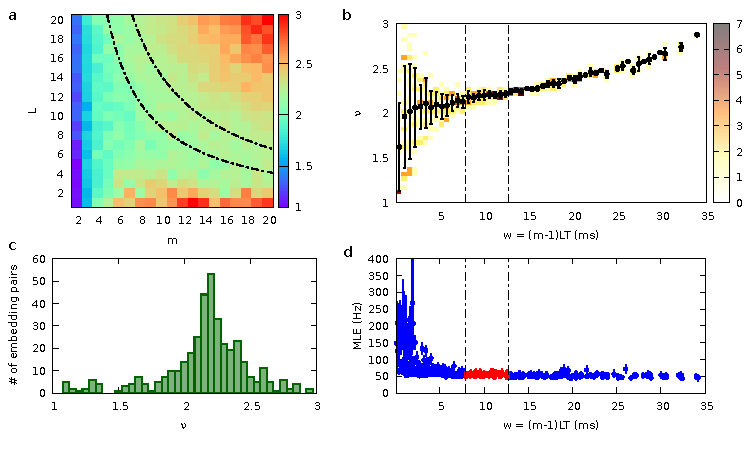
\includegraphics[width=\linewidth]{../2_blocks/1e5_points/plots/chaos.pdf}
    \caption{ciao}
    \label{fig:2 blocks chaos}
\end{figure}


\subsection{Three blocks}

\begin{figure}[H]
    \centering
    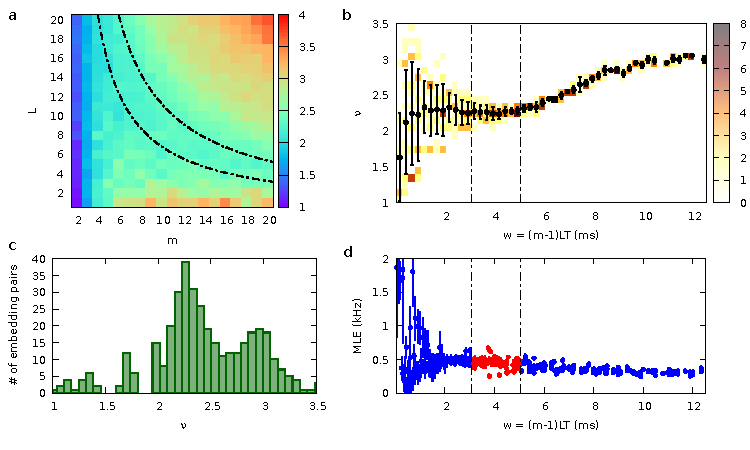
\includegraphics[width=\linewidth]{../3_blocks/2e5_points/plots/chaos_low.pdf}
    \caption{ciao}
    \label{fig:3 blocks chaos}
\end{figure}

\subsection{Four blocks}

\begin{figure}[H]
    \centering
    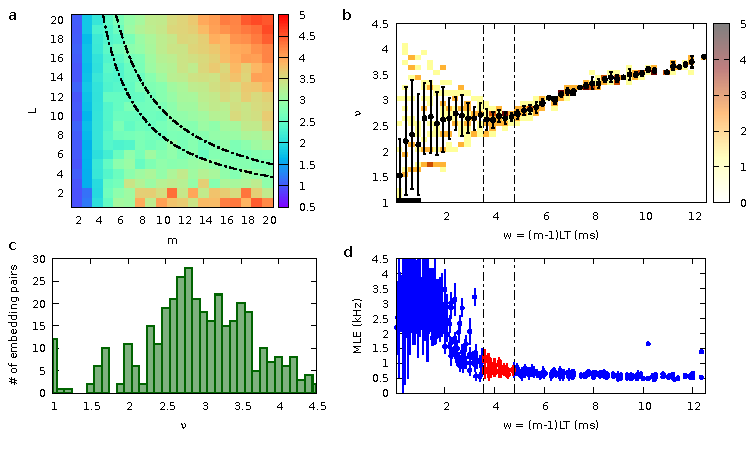
\includegraphics[width=\linewidth]{../4_blocks/2e5_points/plots/chaos_low.pdf}
    \caption{ciao}
    \label{fig:4 blocks chaos}
\end{figure}


\subsection{Five blocks}

\begin{figure}[H]
    \centering
    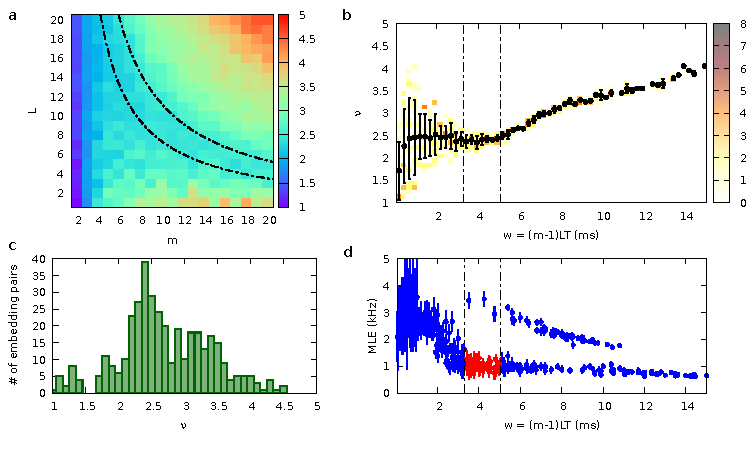
\includegraphics[width=\linewidth]{../5_blocks/2e5_points/plots/chaos_low.pdf}
    \caption{ciao}
    \label{fig:5 blocks chaos}
\end{figure}

\subsection{Six blocks}

\begin{figure}[H]
    \centering
    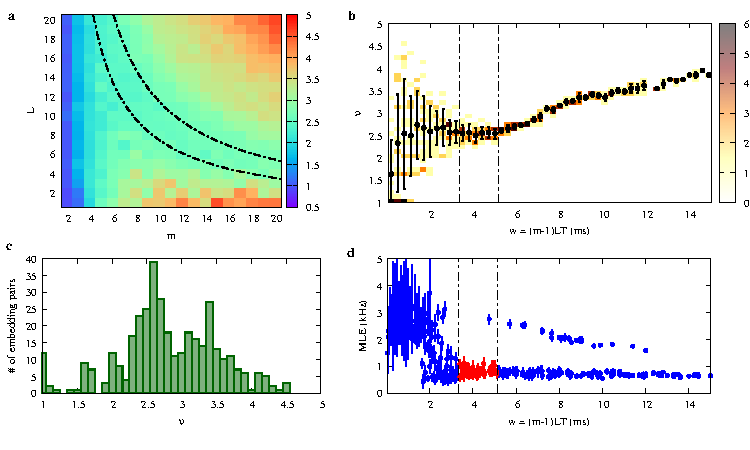
\includegraphics[width=\linewidth]{../6_blocks/2e5_points/plots/chaos_low.pdf}
    \caption{ciao}
    \label{fig:6 blocks chaos}
\end{figure}

\subsection{Seven blocks}

\begin{figure}[H]
    \centering
    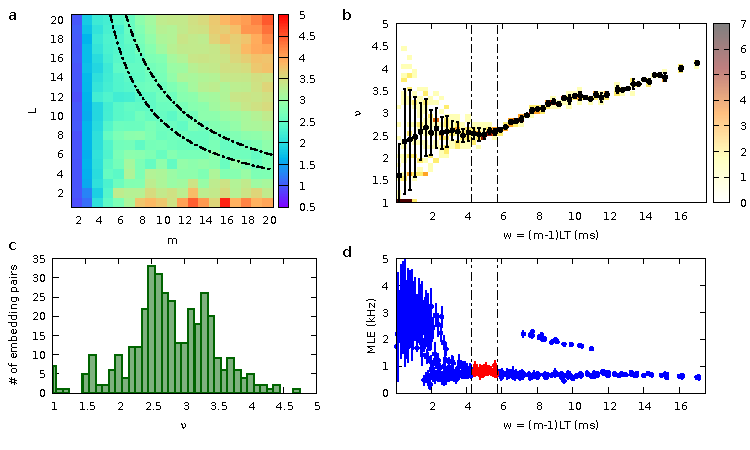
\includegraphics[width=\linewidth]{../7_blocks/2e5_points/plots/chaos_low.pdf}
    \caption{ciao}
    \label{fig:7 blocks chaos}
\end{figure}

\subsection{Eight blocks}

\begin{figure}[H]
    \centering
    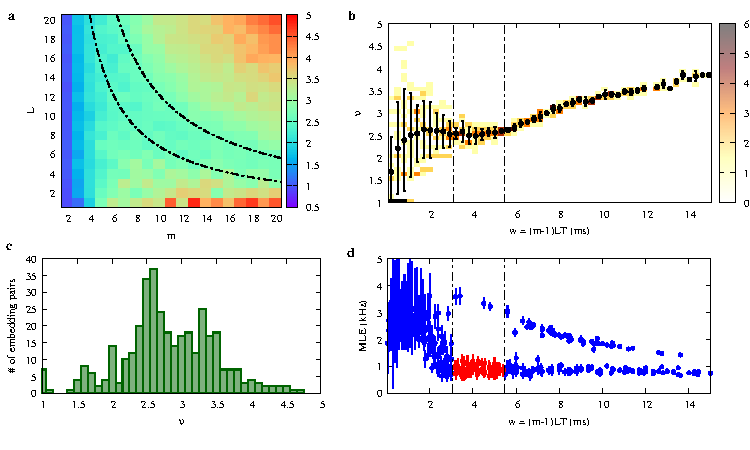
\includegraphics[width=\linewidth]{../8_blocks/2e5_points/plots/chaos_low.pdf}
    \caption{ciao}
    \label{fig:8 blocks chaos}
\end{figure}

\subsection{Nine blocks}

\begin{figure}[H]
    \centering
    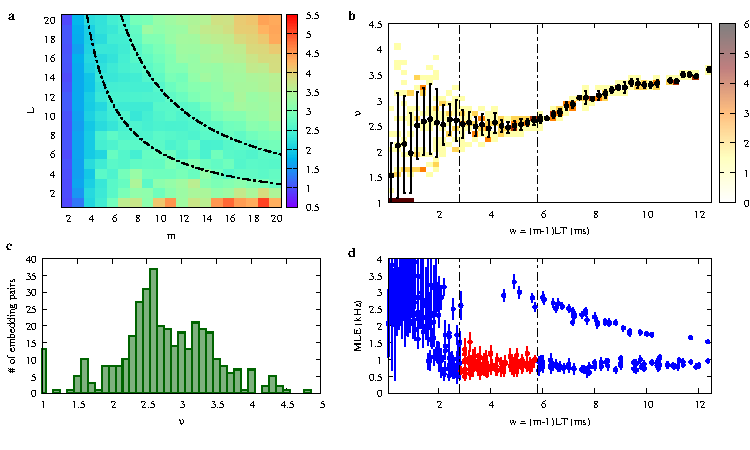
\includegraphics[width=\linewidth]{../9_blocks/edge/2e5_points/plots/chaos_low.pdf}
    \caption{Edge}
    \label{fig:9 blocks chaos}
\end{figure}

\begin{figure}[H]
    \centering
    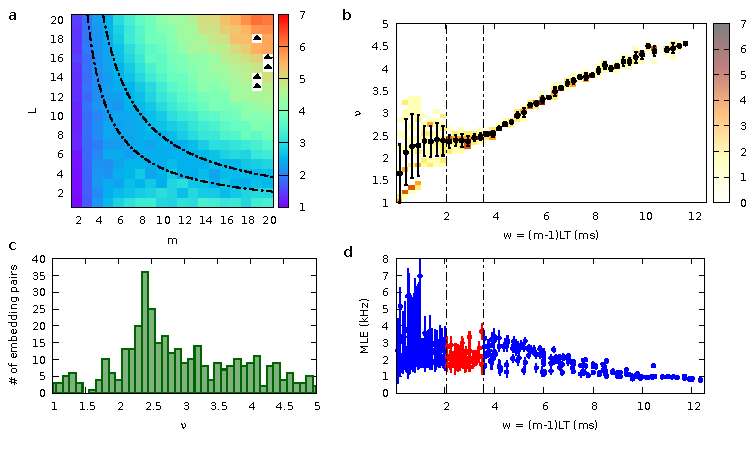
\includegraphics[width=\linewidth]{../9_blocks/middle/2e5_points/plots/chaos_low.pdf}
    \caption{Middle}
    \label{fig:9 blocks chaos middle}
\end{figure}

\subsection{Ten blocks}

\begin{figure}[H]
    \centering
    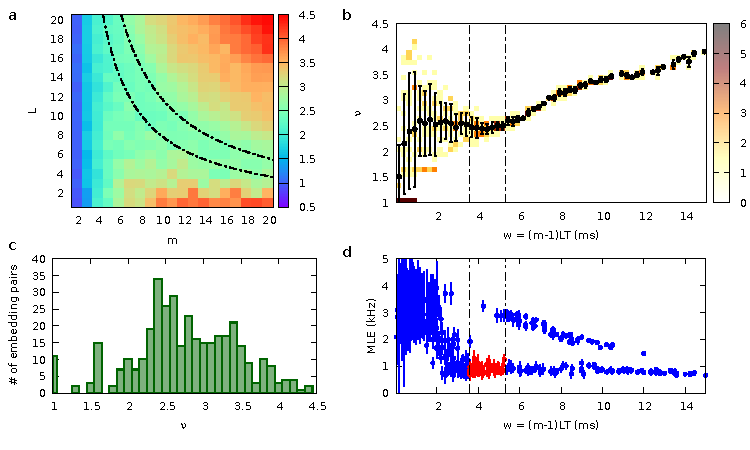
\includegraphics[width=\linewidth]{../10_blocks/2e5_points/plots/chaos_low.pdf}
    \caption{ciao}
    \label{fig:10 blocks chaos}
\end{figure}

\subsection{Conclusions}

\begin{figure}[H]
    \centering
    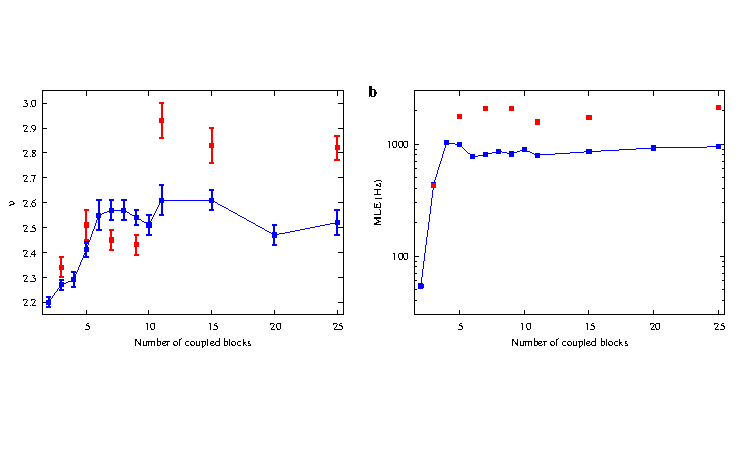
\includegraphics[width=\linewidth,trim={0 1.5cm 0 1.3cm},clip]
    {../data/nu_mle_blocks.pdf}
    \caption{ciao}
    \label{fig:nu mle blocks}
\end{figure}

\clearpage

\printbibliography

\end{document}
